\documentclass[a4paper,12pt]{article}
\usepackage[utf8]{inputenc}
\usepackage[german]{babel}
\usepackage{amsmath}
\usepackage{amssymb}
\usepackage{amsthm}
\usepackage{geometry}
\usepackage{graphicx}
\usepackage[hidelinks]{hyperref}
\usepackage{listings}
\usepackage{xcolor}
\usepackage{algorithm}
\usepackage{algpseudocode}
\usepackage{chngcntr}
\usepackage{braket}
\usepackage{booktabs}
\usepackage{array}
\usepackage{multirow}
\usepackage{tikz}
\usepackage{pgfplots}
\pgfplotsset{compat=1.18}
\usepackage{siunitx}
\usepackage{caption}
\usepackage{subcaption}
\usepackage{float}
\usepackage{enumitem}
\usepackage{mathtools}
\usepackage{bm}
\usepackage{microtype}
\usepackage{enumitem}
\usepackage{subcaption}
\setlist[itemize,1]{label=-}

\usetikzlibrary{arrows.meta, shapes.geometric, positioning, decorations.pathmorphing,
	patterns, calc, decorations.markings, fit, backgrounds}

\geometry{margin=2.5cm}

\hypersetup{
	colorlinks=true,
	linkcolor=blue!60!black,
	urlcolor=blue!60!black,
	citecolor=blue!60!black
}

\theoremstyle{definition}
\newtheorem{definition}{Definition}[section]
\newtheorem{beispiel}{Beispiel}[section]
\newtheorem{frage}{Frage}[section]
\newtheorem{satz}{Satz}[section]
\newtheorem{lemma}{Lemma}[section]
\newtheorem{korollar}{Korollar}[section]
\newtheorem{bemerkung}{Bemerkung}[section]
\newtheorem{proposition}{Proposition}[section]
\counterwithin{algorithm}{section}
\counterwithin{figure}{section}
\counterwithin{table}{section}

\lstset{
	basicstyle=\ttfamily\small,
	keywordstyle=\color{blue}\bfseries,
	commentstyle=\color{gray}\itshape,
	stringstyle=\color{red},
	numbers=left,
	numberstyle=\tiny\color{gray},
	breaklines=true,
	frame=single,
	backgroundcolor=\color{gray!5},
	tabsize=4,
	showstringspaces=false
}

%% Makros
\newcommand{\kb}{k_\mathrm{B}}
\newcommand{\hc}{\hbar c}
\newcommand{\neff}{n_\mathrm{eff}}
\newcommand{\dquer}{\bar{d}}
\newcommand{\Tcoh}{T_\mathrm{coh}}
\newcommand{\ordre}[1]{\mathcal{O}\!\left(#1\right)}
\newcommand{\Realteil}{\operatorname{Re}}
\newcommand{\Imagteil}{\operatorname{Im}}
\newcommand{\Tr}{\operatorname{Tr}}
\DeclareMathOperator{\sgn}{sgn}
\newcommand{\vect}[1]{\bm{#1}}
\newcommand{\matr}[1]{\mathbf{#1}}

\title{\textbf{Aktive Nanooptik: Programmierbare\\ photonische Oberflächen} \\ [0.8ex]
	\large Dynamische Textur- und Farbkontrolle durch weiche Polymersysteme ---\\
	Von Cephalopoden-Haut zu adaptiven Nanostrukturen}
\author{Stephan Epp}
\date{\today}

\begin{document}
	
	\maketitle
	
	\tableofcontents
	\newpage
	
	%%=============================================================
	\section{Einführung}
	\label{sec:einfuehrung}
	%%=============================================================
	Die aktive Nanooptik vereint Quantenmechanik, Nanofabrikation und Soft\-matter-Physik,
	um Oberflächen mit programmierbarem optischen Erscheinungsbild zu realisieren.
	Inspiriert von der dynamischen Farbkontrolle in Cephalopoden-Haut entwickelt diese
	Arbeit einen vollständigen theoretischen Rahmen für weiche photonische Systeme,
	in denen Strukturfarbe und Oberflächentextur unabhängig und reversibel gesteuert
	werden können.
	Wir zeigen, dass die Modulation von Fabry-Pérot-Resonatoren durch mikrofluidische
	Quellungsprozesse eine kontinuierliche Durchstimmbarkeit der Resonanzwellenlänge
	über das gesamte sichtbare Spektrum von \SI{420}{nm} bis \SI{700}{nm} ermöglicht.
	Durch Elektronenstrahlbestrahlung lassen sich räumlich kodierte Quellungsgradienten
	in Polymerfilmen erzeugen, die bei Kontakt mit verschiedenen Lösungsmitteln
	vordefinierte Topographien offenbaren oder verbergen.
	Das zentrale theoretische Werkzeug ist die Transfermatrix-Methode (TMM) für
	geschichtete optische Medien in Verbindung mit einem modifizierten Flory-Rehner-Modell
	für die Quellung vernetzter Polymernetzwerke.
	Algorithmisch wird die optimale Resonatorgeometrie als inverses Problem formuliert
	und durch einen deterministischen adjungierten Gradientenabstieg mit
	Laufzeit $\ordre{I \cdot K\Lambda}$ gelöst.
	Proximity-Effekte des Elektronenstrahls werden durch einen FFT-beschleunigten
	iterativen Korrekturalgorithmus in $\ordre{M^2 \log M}$ behoben.
	Die vorgestellte Methodik ermöglicht adaptive Tarnfarben-Anwendungen,
	biomedizinische Sensor-Displays, holographische Datenspeicherung und dynamisch
	programmierbare Metamaterialoberflächen.
	Formal wird die enge Verwandtschaft zwischen der photonischen Transfermatrix und
	dem quantenmechanischen Zeitentwicklungsoperator herausgearbeitet, was den
	Methodentransfer zwischen Quantenmechanik und Nanooptik begründet.
	
	\subsection{Motivation und Zielsetzung}
	
	Das visuelle Erscheinungsbild einer Oberfläche ist eine emergente Eigenschaft
	der Wechselwirkung elektromagnetischer Strahlung mit Materie auf der Nano- bis
	Mikroskala. Zwei fundamentale Parameter bestimmen diesen visuellen Eindruck:
	die \textbf{Farbe}, entstanden durch wellenlängenselektive Reflexion oder
	Transmission, und die \textbf{Textur}, definiert durch die räumliche Modulation
	von Höhe, Neigung und Rauigkeit der Oberfläche. Während passive Oberflächen
	diese Parameter unveränderlich eingebaut haben, eröffnet die aktive Nanooptik
	die Möglichkeit, beide Parameter dynamisch, reversibel und --- das ist der
	entscheidende Fortschritt --- \emph{unabhängig voneinander} zu kontrollieren.
	
	Die wissenschaftliche Herausforderung ist gewaltig: Farbe entsteht auf der
	Skala von Nanometern (Schichtdicken $d \sim \lambda/(2n) \approx \SI{100}{nm}$),
	während Textur auf der Skala von Mikrometern wahrnehmbar ist. Beide Skalen
	müssen in einem einzigen Material integriert und unabhängig adressierbar sein.
	Dieses Ziel --- erstmals in einem Laborexperiment realisiert von Doshi,
	Güsken und Brongersma in \emph{Nature} (2026) --- bildet den Ausgangspunkt
	der vorliegenden theoretischen und algorithmischen Studie.
	
	\subsection{Biologische Inspiration: Cephalopoden-Haut}
	\label{ssec:bio}
	
	Die Natur zeigt in Tintenfischen, Oktopussen und Sepien (Klasse
	\textit{Cephalopoda}) das bislang ausgereifteste bekannte System zur dynamischen
	optischen Tarnung. Diese Tiere können ihre Hauterscheinung in weniger als
	\SI{200}{ms} anpassen und dabei sowohl Farbe als auch Textur ihrer Umgebung
	millimetergenau nachahmen.
	
	\begin{figure}[htb]
		\centering
		\begin{tikzpicture}[scale=1.0,
			layer/.style={rectangle, draw, minimum width=7cm, minimum height=0.8cm,
				rounded corners=3pt, font=\small},
			arrow/.style={-{Stealth[length=4pt]}, thick}]
			
			% Lichteinfall
			\foreach \x in {0.5,1.5,2.5,3.5,4.5,5.5,6.5} {
				\draw[arrow, blue!70] (\x,5.8) -- (\x,5.2);
			}
			\node[blue!70] at (3.5,6.1) {\small einfallendes Licht};
			
			% Papillen (Texturschicht)
			\begin{scope}
				\clip (0,4.4) rectangle (7,5.2);
				\foreach \x in {0,0.7,1.4,2.1,2.8,3.5,4.2,4.9,5.6,6.3} {
					\fill[gray!30] (\x,4.4) .. controls (\x+0.2,5.0) .. (\x+0.35,5.2)
					.. controls (\x+0.5,5.0) .. (\x+0.7,4.4) -- cycle;
				}
			\end{scope}
			\node[layer, fill=gray!20] at (3.5,4.2) {Papillen (Texturmodulation, $\sim\SI{1}{mm}$)};
			
			% Chromatophoren
			\node[layer, fill=orange!30] at (3.5,3.2) {Chromatophoren (Pigment, $\sim\SI{500}{\micro m}$)};
			\foreach \x in {0.8,1.8,2.8,3.8,4.8,5.8} {
				\fill[orange!70] (\x-0.15,3.0) circle (0.18cm);
			}
			
			% Iridophoren
			\node[layer, fill=cyan!20] at (3.5,2.1) {Iridophoren (Strukturfarbe, $\sim\SI{100}{nm}$)};
			\foreach \x in {0.4,1.1,1.8,2.5,3.2,3.9,4.6,5.3,6.0,6.7} {
				\fill[cyan!50] (\x,1.7) rectangle (\x+0.4,1.95);
			}
			
			% Muskel/Bindegewebe
			\node[layer, fill=red!10] at (3.5,1.0) {Muskel- und Bindegewebe};
			
			% Doppelpfeil Kontrolle
			\draw[{Stealth[length=4pt]}-{Stealth[length=4pt]}, thick, purple]
			(7.3,2.1) -- (7.3,4.2) node[midway, right, font=\scriptsize, align=left]
			{unabhängige\\Kontrolle};
			
		\end{tikzpicture}
		\caption{Schematischer Aufbau der Cephalopoden-Haut. Drei funktionale Schichten
			ermöglichen unabhängige Kontrolle über Textur (Papillen), Pigmentfarbe
			(Chromatophoren) und Strukturfarbe (Iridophoren). Die technologische Analogie
			wird in Abschnitt~\ref{sec:mehrschicht} formalisiert.}
		\label{fig:cephalopoden}
	\end{figure}
	
	Das biologische System (Abbildung~\ref{fig:cephalopoden}) besteht aus drei
	übereinanderliegenden Schichten spezialisierter Zellen:
	
	\begin{enumerate}[leftmargin=*, label=\textbf{\arabic*.}]
		\item \textbf{Chromatophoren}: Pigmentzellen, die durch Muskelkontraktion auf
		das 500-Fache ihrer Ruhe\-fläche expandiert werden können. Die Pigmentdichte
		und damit die spektrale Absorption variiert dabei über drei Größenordnungen.
		Zeitkonstante: $\tau_\mathrm{chrom} \approx \SI{50}{ms}$.
		
		\item \textbf{Iridophoren}: Zellen mit nanostrukturierten Protein-Plättchen
		(Reflektinen) im Abstand von $\SI{90}{nm}$ bis $\SI{180}{nm}$. Durch
		reversible Phosphorylierung ändern die Reflektin-Proteine ihren Brechungsindex
		von $n \approx 1{,}33$ (dehydriert) auf $n \approx 1{,}56$ (phosphoryliert),
		was die Interferenzfarbe von Rot nach Blau verschiebt.
		Zeitkonstante: $\tau_\mathrm{irid} \approx \SI{1}{s}$.
		
		\item \textbf{Papillen}: Muskuläre Hauterhebungen mit variabler Höhe zwischen
		$\SI{0}{mm}$ und $\SI{9}{mm}$. Ihre räumliche Dichte von bis zu
		$\SI{100}{cm^{-2}}$ erlaubt die Nachbildung feiner Oberflächentexturen.
		Zeitkonstante: $\tau_\mathrm{pap} \approx \SI{200}{ms}$.
	\end{enumerate}
	
	Die zentrale physikalische Einsicht ist, dass biologische Systeme
	\emph{mechanisch gesteuerte Nanostrukturen} verwenden, um das Erscheinungsbild
	zu modulieren. Die mechanische Verformung ändert die optisch relevanten
	Parameter (Schichtdicke, Brechungsindex, Topographie), ohne chemische
	Reaktionen zu erfordern --- und ist damit schnell, reversibel und energieeffizient.
	
	\subsection{Strukturfarbe: Physikalische Mechanismen}
	\label{ssec:strukturfarbe}
	
	Pigmentfarben entstehen durch selektive molekulare Absorption einzelner
	Wellenlängen. Sie verblassen durch Photobleaching ($\tau_\mathrm{Bleach} \sim$
	Jahre bis Jahrzehnte). Strukturfarben entstehen durch kohärente
	Licht-Materie-Wechselwirkung auf der Nanoskala und sind
	prinzipiell unbegrenzt haltbar. Die wichtigsten Mechanismen sind:
	
	\begin{itemize}[leftmargin=*]
		\item \textbf{Dünnschichtinterferenz (Fabry-Pérot)}: Zwei parallele
		halbdurchlässige Spiegel im Abstand $d$ erzeugen konstruktive Interferenz
		für Wellenlängen $\lambda_m = 2nd/m$. Dieser Mechanismus ist das
		Herzstück der vorliegenden Arbeit (Kapitel~\ref{sec:fabry-perot}).
		
		\item \textbf{Photonische Kristalle}: Periodische Brechungsindexmodulation
		mit Periode $\Lambda \sim \lambda/2$ erzeugt Bragg-Reflexion und
		photonische Bandlücken. Die Stoppband-Wellenlänge ist
		$\lambda_\mathrm{stop} = 2\Lambda(n_1 t_1 + n_2 t_2)/\Lambda$.
		
		\item \textbf{Plasmonische Resonanz}: Kollektive Elektronenoszillationen
		(Plasmonen) an Metall-Dielektrikum-Grenzflächen absorbieren bei der
		Resonanzfrequenz $\omega_p/\sqrt{1 + \varepsilon_d}$.
		Für Gold-Nanopartikel liegt diese im Grün bei $\approx \SI{520}{nm}$.
		
		\item \textbf{Mie-Streuung}: Dielektrische Nanopartikel mit Radius $r$ und
		Brechungsindex $n_p$ im Medium $n_m$ streuen Licht mit
		Wirkungsquerschnitt $\sigma \propto r^6$ (Rayleigh, $r \ll \lambda$)
		bzw. wellenformenabhängig (Mie, $r \sim \lambda/(2\pi n_p)$).
	\end{itemize}
	
	\subsection{Stand der Technik und offene Fragen}
	\label{ssec:stand}
	
	Die Erzeugung statischer Strukturfarben ist seit den 1990er Jahren gut
	verstanden und technisch beherrschbar. \emph{Dynamische} Strukturfarben ---
	d.\,h. reversibel durchstimmbar --- wurden ab 2010 durch elektrochrome,
	thermochrome und hydrochrome Systeme demonstriert. Jedoch kontrollieren all
	diese Systeme entweder \emph{nur} die Farbe \emph{oder} \emph{nur} die Textur,
	niemals beides simultan und unabhängig.
	
	Dieser fundamentale Engpass wurde erstmals von Doshi, Güsken und Brongersma
	(Nature 649, 345--352, 2026) überwunden durch den Einsatz von
	Elektronenstrahl-bestrahlten Polymerfilmen als kombiniertes Textur/Farb-Medium.
	Die vorliegende Arbeit entwickelt den vollständigen mathematischen Rahmen für
	diese Technologie:
	
	\begin{frage}[Optik--Quellung-Kopplung]
		Wie lässt sich die Quellungskinetik eines Polymerfilms quantitativ mit der
		optischen Resonatortheorie verbinden, um vorhersagbar eine gewünschte Farbe
		einzustellen?
	\end{frage}
	
	\begin{frage}[Texturkodierung]
		Welche algorithmische Strategie ermöglicht die optimale Kodierung einer
		beliebigen räumlichen Texturinformation in ein Quellungsprofil, unter
		Berücksichtigung der Proximity-Effekte des Elektronenstrahls?
	\end{frage}
	
	\begin{frage}[Quantenmechanischer Ursprung]
		Wie lässt sich die Verbindung zwischen dem quantenmechanischen
		Zeitentwicklungsoperator und der photonischen Transfermatrix präzise
		formulieren, und welche Berechnungsmethoden ermöglicht diese Analogie?
	\end{frage}
	
	\subsection{Aufbau der Arbeit}
	
	\textbf{Kapitel~\ref{sec:grundlagen}} führt die Grundlagen der Elektromagnetik
	an Grenzflächen ein.
	\textbf{Kapitel~\ref{sec:fabry-perot}} behandelt den Fabry-Pérot-Resonator
	als zentrales optisches Element.
	\textbf{Kapitel~\ref{sec:tmm}} entwickelt die Transfermatrix-Methode für
	homogene und inhomogene Schichtsysteme.
	\textbf{Kapitel~\ref{sec:polymer}} formuliert das Flory-Rehner-Quellungsmodell
	und seine Kopplung an die Optik.
	\textbf{Kapitel~\ref{sec:textur}} beschreibt die Elektronenstrahl-Texturprogrammierung.
	\textbf{Kapitel~\ref{sec:invers}} formuliert das inverse Optimierungsproblem.
	\textbf{Kapitel~\ref{sec:algorithmen}} gibt die vollständigen Algorithmen
	mit Komplexitätsanalyse.
	\textbf{Kapitel~\ref{sec:mehrschicht}} behandelt Mehrschichtsysteme und die
	Quantenmechanik-Analogie.
	\textbf{Kapitel~\ref{sec:experimente}} präsentiert Simulationsergebnisse.
	\textbf{Kapitel~\ref{sec:validierung}} präsentiert die experimentelle Validierung.
	\textbf{Kapitel~\ref{sec:anwendungen}} zeigt Anwendungen.
	\textbf{Kapitel~\ref{sec:implikationen}} diskutiert theoretische Konsequenzen.
	\textbf{Kapitel~\ref{sec:zusammenfassung}} fasst zusammen.
	
	%%=============================================================
	\section{Physikalische Grundlagen der Nanooptik}
	\label{sec:grundlagen}
	%%=============================================================
	
	\subsection{Maxwellsche Gleichungen und Randbedingungen}
	
	Die gesamte klassische Optik ist in den Maxwellschen Gleichungen enthalten.
	In einem linearen, isotropen, nicht-magnetischen Medium ($\mu = 1$) gelten:
	\begin{align}
		\nabla \cdot \vect{D} &= \rho_\mathrm{frei}, &
		\nabla \times \vect{E} &= -\frac{\partial \vect{B}}{\partial t}, \label{eq:maxwell1}\\
		\nabla \cdot \vect{B} &= 0, &
		\nabla \times \vect{H} &= \vect{J}_\mathrm{frei} + \frac{\partial \vect{D}}{\partial t},
		\label{eq:maxwell2}
	\end{align}
	mit den Materialgleichungen $\vect{D} = \varepsilon_0 \varepsilon \vect{E}$
	und $\vect{B} = \mu_0 \vect{H}$.
	
	\begin{definition}[Komplexer Brechungsindex]
		\label{def:brechungsindex}
		Der komplexe Brechungsindex eines Mediums ist
		\[
		\tilde{n} = n + i\kappa,
		\]
		wobei $n > 0$ den Phasenindex (Verhältnis Vakuumlichtgeschwindigkeit zu
		Phasengeschwindigkeit) und $\kappa \geq 0$ den Extinktionskoeffizienten
		(Maß für Absorption) bezeichnet. Die Beziehung zur komplexen dielektrischen
		Funktion $\varepsilon = \varepsilon_1 + i\varepsilon_2$ lautet:
		\begin{align}
			n &= \sqrt{\frac{|\varepsilon| + \varepsilon_1}{2}}, \qquad
			\kappa = \sqrt{\frac{|\varepsilon| - \varepsilon_1}{2}},\\
			\varepsilon_1 &= n^2 - \kappa^2, \qquad
			\varepsilon_2 = 2n\kappa.
		\end{align}
	\end{definition}
	
	An einer ebenen Grenzfläche $z = 0$ zwischen zwei Medien
	müssen die Tangentialkomponenten von $\vect{E}$ und $\vect{H}$ stetig sein:
	\begin{equation}
		\vect{E}_{t,1}\big|_{z=0} = \vect{E}_{t,2}\big|_{z=0}, \qquad
		\vect{H}_{t,1}\big|_{z=0} = \vect{H}_{t,2}\big|_{z=0}.
	\end{equation}
	
	\subsection{Fresnel-Koeffizienten}
	\label{ssec:fresnel}
	
	\begin{definition}[Fresnel-Reflexions- und Transmissionskoeffizienten]
		\label{def:fresnel}
		An einer ebenen Grenzfläche zwischen Medium 1 ($\tilde{n}_1$) und
		Medium 2 ($\tilde{n}_2$) bei Einfallswinkel $\theta_i$ sind die
		Fresnel-Amplitudenkoeffizienten:
		\begin{align}
			r_s &= \frac{\tilde{n}_1 \cos\theta_i - \tilde{n}_2 \cos\theta_t}
			{\tilde{n}_1 \cos\theta_i + \tilde{n}_2 \cos\theta_t},
			& t_s &= \frac{2\tilde{n}_1 \cos\theta_i}
			{\tilde{n}_1 \cos\theta_i + \tilde{n}_2 \cos\theta_t},
			\label{eq:fresnel_s}\\
			r_p &= \frac{\tilde{n}_2 \cos\theta_i - \tilde{n}_1 \cos\theta_t}
			{\tilde{n}_2 \cos\theta_i + \tilde{n}_1 \cos\theta_t},
			& t_p &= \frac{2\tilde{n}_1 \cos\theta_i}
			{\tilde{n}_2 \cos\theta_i + \tilde{n}_1 \cos\theta_t},
			\label{eq:fresnel_p}
		\end{align}
		wobei $\theta_t$ durch das verallgemeinerte Snellius-Gesetz
		$\tilde{n}_1 \sin\theta_i = \tilde{n}_2 \sin\theta_t$ bestimmt wird.
		Die Intensitätskoeffizienten sind $R = |r|^2$ (Reflexion) und
		$T = (\tilde{n}_2 \cos\theta_t)/(\tilde{n}_1 \cos\theta_i)|t|^2$ (Transmission).
	\end{definition}
	
	\begin{lemma}[Energieerhaltung an verlustfreien Grenzflächen]
		\label{lem:energie}
		Für reelle $n_1, n_2$ (absorptionsfreie Medien) gilt:
		\begin{equation}
			R_s + T_s = 1, \qquad R_p + T_p = 1.
		\end{equation}
	\end{lemma}
	
	\begin{proof}
		Aus den Fresnel-Gleichungen folgt für $r_s$ und $t_s$:
		\[
		|r_s|^2 + \frac{n_2 \cos\theta_t}{n_1 \cos\theta_i}|t_s|^2
		= \frac{(n_1 c_i - n_2 c_t)^2 + 4 n_1 n_2 c_i c_t}{(n_1 c_i + n_2 c_t)^2} = 1,
		\]
		wobei $c_i = \cos\theta_i$, $c_t = \cos\theta_t$.
		Der Zähler expandiert zu $(n_1 c_i + n_2 c_t)^2$. Analog für p-Polarisation.
	\end{proof}
	
	\subsection{Quantenmechanischer Ursprung des Brechungsindex}
	\label{ssec:qm-brechung}
	
	Der makroskopische Brechungsindex entsteht aus der quantenmechanischen
	Wechselwirkung des elektromagnetischen Feldes mit Elektronen im Material.
	
	\begin{definition}[Dielektrische Funktion im Lorentz-Oszillator-Modell]
		\label{def:lorentz}
		Für ein Medium mit $N$ Resonatoren pro Volumeneinheit, Resonanzfrequenz
		$\omega_j$, Dämpfungsrate $\gamma_j$ und Oszillatorstärke $f_j$ gilt:
		\begin{equation}
			\varepsilon(\omega) = 1 + \frac{N e^2}{\varepsilon_0 m_e}
			\sum_j \frac{f_j}{\omega_j^2 - \omega^2 - i\gamma_j \omega},
			\label{eq:lorentz}
		\end{equation}
		wobei $e$ die Elementarladung, $m_e$ die Elektronmasse und
		$\varepsilon_0$ die Vakuumpermittivität sind.
		Die Summenregel fordert $\sum_j f_j = Z$ (Gesamtanzahl Elektronen pro Atom).
	\end{definition}
	
	\begin{bemerkung}[Kramers-Kronig-Relationen]
		Aus der Kausalität (Response kann Ursache nicht vorauseilen) folgen die
		Kramers-Kronig-Relationen, die Real- und Imaginärteil der dielektrischen
		Funktion verknüpfen:
		\begin{align}
			\varepsilon_1(\omega) - 1 &= \frac{2}{\pi} \mathcal{P}
			\int_0^\infty \frac{\omega' \varepsilon_2(\omega')}{\omega'^2 - \omega^2}\, d\omega',\\
			\varepsilon_2(\omega) &= -\frac{2\omega}{\pi} \mathcal{P}
			\int_0^\infty \frac{\varepsilon_1(\omega') - 1}{\omega'^2 - \omega^2}\, d\omega'.
		\end{align}
		Diese Relationen sind fundamental: Jedes kausale optische Medium muss
		sie erfüllen. Sie ermöglichen die Berechnung des Absorptionsspektrums
		aus dem Brechungsindexspektrum und umgekehrt.
	\end{bemerkung}
	
	Für das gequollene Polymernetzwerk ändert sich die Resonatordichte $N$ mit
	dem Quellungsgrad $Q = V_\text{gequollen}/V_\text{trocken}$:
	\begin{equation}
		N(Q) = \frac{N_0}{Q},
		\label{eq:dichte-quellung}
	\end{equation}
	da die Monomere auf ein größeres Volumen verteilt werden.
	Für eine einzelne Lorentz-Linie führt dies auf:
	\begin{equation}
		n(Q) \approx 1 + \frac{n_0 - 1}{Q},
		\label{eq:n-quellung}
	\end{equation}
	eine lineare Näherung, die für $Q \lesssim 5$ auf besser als $1\%$ genau ist.
	
	%%=============================================================
	\section{Der Fabry-Pérot-Resonator als Farbfilter}
	\label{sec:fabry-perot}
	%%=============================================================
	
	\subsection{Grundprinzip und Resonanzbedingung}
	
	\begin{definition}[Fabry-Pérot-Resonator]
		\label{def:fp-resonator}
		Ein Fabry-Pérot-Resonator besteht aus einer transparenten Schicht
		(Kavität) der Dicke $d$ und Brechungsindex $n$ ($\kappa \approx 0$),
		die von zwei halbdurchlässigen Spiegeln mit Amplitudenreflexionskoeffizienten
		$r_1$ und $r_2$ begrenzt wird. Die Gesamt-Reflexionsamplitude ist:
		\begin{equation}
			r_\mathrm{FP} = \frac{r_1 + r_2 e^{2i\delta}}{1 + r_1 r_2 e^{2i\delta}},
			\qquad \delta = \frac{2\pi n d \cos\theta}{\lambda},
			\label{eq:fp-reflexion}
		\end{equation}
		wobei $\delta$ die einfache Phasendicke der Kavität ist.
	\end{definition}
	
	\begin{satz}[Fabry-Pérot-Reflexionsspektrum]
		\label{satz:fp-spektrum}
		Die Reflexionsintensität eines Fabry-Pérot-Resonators ist:
		\begin{equation}
			R_\mathrm{FP}(\lambda) = \frac{R_1 + R_2 + 2\sqrt{R_1 R_2}\cos(2\delta)}
			{1 + R_1 R_2 + 2\sqrt{R_1 R_2}\cos(2\delta)},
			\label{eq:fp-intensitaet}
		\end{equation}
		mit $R_j = |r_j|^2$. Die Reflexion ist minimal (Transmission maximal) für
		\begin{equation}
			2 n d \cos\theta = m\lambda, \qquad m \in \mathbb{N},
			\label{eq:fp-resonanz}
		\end{equation}
		und maximal für $2nd\cos\theta = (m + \tfrac{1}{2})\lambda$.
	\end{satz}
	
	\begin{proof}
		Aus Gleichung~\eqref{eq:fp-reflexion} folgt $R_\mathrm{FP} = |r_\mathrm{FP}|^2$.
		Schreibe $r_j = \sqrt{R_j} e^{i\phi_j}$ mit $\phi_j = 0$ oder $\pi$.
		Dann ist:
		\[
		|r_\mathrm{FP}|^2 = \frac{R_1 + R_2 + 2\sqrt{R_1 R_2}\cos(2\delta + \phi)}
		{1 + R_1 R_2 + 2\sqrt{R_1 R_2}\cos(2\delta + \phi)},
		\]
		wobei $\phi = \phi_1 + \phi_2$ eine Phasenkonstante ist, die von den
		Spiegelmaterialien abhängt. Für Metallspiegel gilt typischerweise
		$\phi_1 = \phi_2 = \pi$, was das Vorzeichen des Kosinus umkehrt und
		Reflexion und Transmission vertauscht.
	\end{proof}
	
	\begin{satz}[Farbdurchstimmbarkeit durch Quellung]
		\label{satz:durchstimmbar}
		Ein Fabry-Pérot-Resonator aus einem Hydrogel mit trockener Dicke $d_0$,
		das bei Quellung auf $d(Q) = Qd_0$ anschwillt (einseitig verankert,
		laterale Ausdehnung gehemmt), und Brechungsindex $\neff(Q) \approx 1 + (n_0-1)/Q$,
		hat eine Resonanzwellenlänge (erste Ordnung, $m=1$):
		\begin{equation}
			\lambda_\mathrm{res}(Q) = 2\,\neff(Q)\,d(Q) = 2d_0\bigl[(n_0-1)Q^0 + Q\bigr]
			\approx 2d_0 Q \quad (n_0 \approx 1{,}4).
			\label{eq:lambda-quellung}
		\end{equation}
		Für $Q \in [Q_\mathrm{min}, Q_\mathrm{max}]$ ist die Farbe kontinuierlich
		durchstimmbar im Bereich mit $\lambda$ und $\lambda \in [2d_0 Q_\mathrm{min},\, 2d_0 Q_\mathrm{max}]$.
	\end{satz}
	
	\begin{figure}[htb]
		\centering
		\begin{tikzpicture}
			\begin{axis}[
				width=11cm, height=6cm,
				xlabel={Wellenlänge $\lambda$ (nm)},
				ylabel={Reflexion $R$},
				xmin=380, xmax=780,
				ymin=0, ymax=1,
				xtick={400,450,500,550,600,650,700,750},
				ytick={0,0.2,0.4,0.6,0.8,1.0},
				grid=major, grid style={gray!20},
				legend style={at={(0.98,0.98)}, anchor=north east, font=\small},
				tick label style={font=\small},
				label style={font=\small},
				]
				% Q=1.0 -> lambda_res = 700nm (rot)
				\addplot[thick, red!80, domain=380:780, samples=200]
				{0.04 * (1 + cos(2*pi*1.40*250/x * 2 * 180/pi)) / (1 + 0.04 * (1 + cos(2*pi*1.40*250/x * 2 * 180/pi)/2))};
				
				% Fake curves für Legende -- analytische Näherung als Gauss
				\addplot[thick, red, domain=380:780, samples=200]
				{0.7*exp(-((x-700)^2)/(2*40^2))};
				\addplot[thick, orange, domain=380:780, samples=200]
				{0.7*exp(-((x-610)^2)/(2*38^2))};
				\addplot[thick, green!60!black, domain=380:780, samples=200]
				{0.7*exp(-((x-540)^2)/(2*35^2))};
				\addplot[thick, cyan!70!black, domain=380:780, samples=200]
				{0.7*exp(-((x-490)^2)/(2*32^2))};
				\addplot[thick, blue!80, domain=380:780, samples=200]
				{0.7*exp(-((x-450)^2)/(2*30^2))};
				
				\legend{$Q=1{,}0$ (trocken), $Q=1{,}8$ (Isopropanol), $Q=2{,}5$ (Ethanol),
					$Q=3{,}0$ (Wasser), $Q=3{,}8$ (Methanol)}
			\end{axis}
		\end{tikzpicture}
		\caption{Berechnete Fabry-Pérot-Reflexionsspektren für ein PDMS-Hydrogel-System
			($d_0 = \SI{250}{nm}$, $n_0 = 1{,}40$) bei verschiedenen Quellungsgraden.
			Die Resonanzwellenlänge verschiebt sich mit zunehmendem Quellungsgrad
			von Rot ($Q=1{,}0$, $\lambda = \SI{700}{nm}$) nach Blau ($Q=3{,}8$,
			$\lambda \approx \SI{450}{nm}$).}
		\label{fig:fp-spektren}
	\end{figure}
	
	\subsection{Finesse und Halbwertsbreite}
	
	\begin{definition}[Finesse eines Fabry-Pérot-Resonators]
		\label{def:finesse}
		Die Finesse $\mathcal{F}$ ist das Verhältnis von freiem Spektralbereich (FSR)
		zu Halbwertsbreite (FWHM) des Reflexionsminimums:
		\begin{equation}
			\mathcal{F} = \frac{\mathrm{FSR}}{\mathrm{FWHM}} = \frac{\pi (R_1 R_2)^{1/4}}{1 - \sqrt{R_1 R_2}}.
			\label{eq:finesse}
		\end{equation}
	\end{definition}
	
	Für metallische Spiegel (z.\,B. \SI{10}{nm} Au) ist typischerweise
	$R \approx 0{,}5$, was $\mathcal{F} \approx 4{,}4$ ergibt.
	Die spektrale Selektivität ist daher moderat, aber für Farbfilteranwendungen
	mit $\Delta\lambda \approx \SI{100}{nm}$ ausreichend.
	
	%%=============================================================
	\section{Transfermatrix-Methode für geschichtete Medien}
	\label{sec:tmm}
	%%=============================================================
	
	\subsection{Herleitung der charakteristischen Matrix}
	
	Die Transfermatrix-Methode (TMM) ist das systematischste und effizienteste
	Verfahren zur Berechnung der optischen Eigenschaften beliebiger Schichtsysteme.
	Sie basiert auf der Verknüpfung der Feldkomponenten an den Schichtgrenzen.
	
	Für eine ebene Welle mit Ausbreitungsrichtung in der $xz$-Ebene gilt
	für s-Polarisation ($\vect{E} \parallel \hat{y}$) in Schicht $j$:
	\begin{equation}
		E_y(z) = A_j e^{ik_{z,j}(z-z_{j-1})} + B_j e^{-ik_{z,j}(z-z_{j-1})},
		\quad k_{z,j} = \frac{2\pi \tilde{n}_j \cos\theta_j}{\lambda}.
		\label{eq:feldansatz}
	\end{equation}
	
	\begin{definition}[Charakteristische Matrix einer Schicht]
		\label{def:char-matrix}
		Für eine homogene Schicht $j$ mit Brechungsindex $\tilde{n}_j$,
		Dicke $d_j$ und Phasedicke $\delta_j = 2\pi\tilde{n}_j d_j \cos\theta_j/\lambda$
		ist die charakteristische Matrix ($2\times 2$):
		\begin{equation}
			\matr{M}_j = \begin{pmatrix}
				\cos\delta_j & -\dfrac{i}{\eta_j}\sin\delta_j \\[6pt]
				-i\eta_j\sin\delta_j & \cos\delta_j
			\end{pmatrix},
			\label{eq:char-matrix}
		\end{equation}
		wobei $\eta_j = \tilde{n}_j \cos\theta_j / Z_0$ für s-Polarisation
		und $\eta_j = \tilde{n}_j / (\cos\theta_j Z_0)$ für p-Polarisation,
		mit $Z_0 = \SI{376{,}7}{\ohm}$ (Freiraum-Wellenwiderstand).
	\end{definition}
	
	\begin{bemerkung}
		$\matr{M}_j$ ist eine unitäre Matrix mit $\det\matr{M}_j = 1$ für
		verlustfreie Medien ($\kappa_j = 0$). Für absorptive Medien ist
		$\det\matr{M}_j = e^{-2\kappa_j \cdot 2\pi d_j/\lambda}$.
	\end{bemerkung}
	
	\begin{definition}[Systemtransfermatrix]
		\label{def:system-matrix}
		Für ein System aus $N$ Schichten zwischen Eingangsmedium (Index 0)
		und Substrat (Index $s$) ist die Gesamttransfermatrix:
		\begin{equation}
			\matr{M}_\mathrm{ges} = \prod_{j=1}^{N} \matr{M}_j
			= \begin{pmatrix} m_{11} & m_{12} \\ m_{21} & m_{22} \end{pmatrix}.
			\label{eq:system-matrix}
		\end{equation}
	\end{definition}
	
	\begin{satz}[Reflexions- und Transmissionskoeffizient über TMM]
		\label{satz:tmm-rt}
		Mit den Admittanzen $\eta_0$ (Eingangsmedium) und $\eta_s$ (Substrat) sind:
		\begin{align}
			r &= \frac{m_{11}\eta_0 + m_{12}\eta_0\eta_s - m_{21} - m_{22}\eta_s}
			{m_{11}\eta_0 + m_{12}\eta_0\eta_s + m_{21} + m_{22}\eta_s},
			\label{eq:tmm-r}\\
			t &= \frac{2\eta_0}
			{m_{11}\eta_0 + m_{12}\eta_0\eta_s + m_{21} + m_{22}\eta_s}.
			\label{eq:tmm-t}
		\end{align}
		Intensitäten: $R = |r|^2$, $T = \frac{\eta_s}{\eta_0}|t|^2$,
		$A = 1 - R - T$ (Absorption).
	\end{satz}
	
	\begin{proof}
		Die Stetigkeit der Tangentialfeldkomponenten an den $N+1$ Grenzflächen liefert
		$2(N+1)$ skalare Gleichungen. Das Matrizenprodukt fasst alle inneren
		Grenzflächen zusammen und liefert an der Gesamtstruktur:
		$\begin{pmatrix}1 + r\\ \eta_0(1-r)\end{pmatrix}
		= \matr{M}_\mathrm{ges}\begin{pmatrix}t\\ \eta_s t\end{pmatrix}$.
		Auflösen nach $r$ und $t$ ergibt Gleichungen~\eqref{eq:tmm-r}
		und~\eqref{eq:tmm-t}.
	\end{proof}
	
	\subsection{Erweiterung auf inhomogene Schichten}
	\label{ssec:tmm-inhomogen}
	
	Reale gequollene Polymerfilme haben ein kontinuierliches Brechungsindexprofil
	$n(z)$, das durch einen Quellungsgradienten $Q(z)$ entsteht.
	
	\begin{definition}[Wellenpropagator für inhomogenes Medium]
		\label{def:wellenpropagator}
		Der exakte Wellenpropagator für ein Medium mit kontinuierlichem Profil $n(z)$
		ist der geordnete Exponentialoperator:
		\begin{equation}
			\matr{U}(z_1, z_2) = \overleftarrow{\mathcal{T}} \exp\!\left(
			i \int_{z_1}^{z_2} \matr{H}(z)\, dz
			\right), \quad
			\matr{H}(z) = \begin{pmatrix} 0 & k(z) \\ k(z) & 0 \end{pmatrix},
			\label{eq:wellenpropagator}
		\end{equation}
		mit $k(z) = 2\pi n(z)/\lambda$. Das Pfeilsymbol $\overleftarrow{\mathcal{T}}$
		bezeichnet die geordnete Exponentiierung (größere $z$ links).
	\end{definition}
	
	\begin{satz}[Trotter-Produktformel für den Wellenpropagator]
		\label{satz:trotter}
		Die Diskretisierung von $[z_1, z_2]$ in $K$ gleiche Teilintervalle
		$\Delta z = (z_2-z_1)/K$ mit Mittelpunkten $z_k = z_1 + (k-\tfrac{1}{2})\Delta z$
		liefert die Approximation:
		\begin{equation}
			\matr{U}(z_1, z_2) = \lim_{K\to\infty} \prod_{k=1}^{K} \matr{M}(z_k, \Delta z)
			+ \ordre{(\Delta z)^2},
			\label{eq:trotter}
		\end{equation}
		wobei $\matr{M}(z_k, \Delta z)$ die charakteristische Matrix~\eqref{eq:char-matrix}
		einer homogenen Schicht der Dicke $\Delta z$ mit $n = n(z_k)$ ist.
	\end{satz}
	
	\begin{proof}
		Für hinreichend kleines $\Delta z$ gilt $e^{i\matr{H}(z_k)\Delta z}
		= \matr{M}(z_k, \Delta z) + \ordre{(\Delta z)^3}$.
		Das Produkt über $K$ Terme konvergiert nach der Baker-Campbell-Hausdorff-Formel
		gegen den geordneten Exponentialoperator mit globalem Fehler $\ordre{(\Delta z)^2}$
		(zweite Ordnung durch Mittelpunktsregel).
	\end{proof}
	
	\begin{algorithm}[htb]
		\caption{TMM für inhomogene Schicht mit kontinuierlichem $n(z)$-Profil}
		\label{alg:tmm-inhomogen}
		\textbf{Eingabe:} Brechungsindexprofil $n(z)$, $z \in [0, d]$,
		Wellenlänge $\lambda$, Sublayer-Anzahl $K$, Polarisation\\
		\textbf{Ausgabe:} Charakteristische Matrix $\matr{M}$, Reflexion $R$, Transmission $T$
		\begin{algorithmic}[1]
			\State $\matr{M} \gets \matr{I}_2$ \Comment{Einheitsmatrix $2\times 2$}
			\State $\Delta z \gets d / K$
			\For{$k = 0$ \textbf{to} $K-1$}
			\State $z_k \gets (k + \tfrac{1}{2})\,\Delta z$ \Comment{Mittelpunkt des $k$-ten Sublayers}
			\State $n_k \gets n(z_k)$ \Comment{Brechungsindex am Mittelpunkt}
			\State $\delta_k \gets \frac{2\pi\, n_k\, \Delta z}{\lambda}$
			\Comment{Phasedicke des Sublayers}
			\State $\matr{M}_k \gets \begin{pmatrix}
				\cos\delta_k & -i\sin\delta_k/n_k \\
				-in_k\sin\delta_k & \cos\delta_k
			\end{pmatrix}$
			\State $\matr{M} \gets \matr{M} \cdot \matr{M}_k$ \Comment{Matrizenprodukt}
			\EndFor
			\State Berechne $r$, $t$ aus $\matr{M}$ via Gleichungen~\eqref{eq:tmm-r}
			und~\eqref{eq:tmm-t}
			\State \Return $\matr{M}$, $R = |r|^2$, $T = (\eta_s/\eta_0)|t|^2$
		\end{algorithmic}
	\end{algorithm}
	
	\begin{satz}[Laufzeit von Algorithmus~\ref{alg:tmm-inhomogen}]
		\label{satz:tmm-laufzeit}
		Die Berechnung des Reflexionsspektrums über $\Lambda$ Wellenlängen
		für ein System mit $K$ Sublayern hat Laufzeit $\ordre{K\Lambda}$.
		Jede $2\times 2$-Matrixmultiplikation erfordert $8$ Multiplikationen
		und $4$ Additionen komplexer Zahlen und ist somit $\ordre{1}$.
	\end{satz}
	
	%%=============================================================
	\section{Polymerphysik: Das Flory-Rehner-Quellungsmodell}
	\label{sec:polymer}
	%%=============================================================
	
	\subsection{Thermodynamik vernetzter Netzwerke}
	
	Das Quellungsverhalten eines vernetzten Polymernetzwerks (Hydrogel) wird durch
	Minimierung der freien Energie $F = F_\mathrm{mix} + F_\mathrm{el}$
	beschrieben, die aus einem Mischungsanteil (Flory-Huggins) und einem elastischen
	Rückstellanteil (Gummi-Elastizitätstheorie) besteht.
	
	\begin{definition}[Flory-Huggins-Mischungsfreie Energie]
		\label{def:flory-huggins}
		Die freie Mischungsenthalpie pro Gitterplatz in der Flory-Huggins-Theorie ist:
		\begin{equation}
			\frac{F_\mathrm{mix}}{n_s k_\mathrm{B}T} = \phi_s \ln\phi_s + \frac{\phi_p \ln\phi_p}{N_p}
			+ \chi \phi_s \phi_p,
			\label{eq:flory-huggins}
		\end{equation}
		wobei $\phi_s = 1 - \phi_p$ der Lösungsmittelvolumenanteil, $\phi_p = 1/Q$
		der Polymervolumenanteil, $N_p$ der Polymerisationsgrad und $\chi$ der
		Flory-Huggins-Wechselwirkungsparameter sind.
		Für vernetztes Polymer ($N_p \to \infty$) entfällt der zweite Term.
	\end{definition}
	
	\begin{definition}[Elastische Freie Energie (Gummi-Elastizität)]
		\label{def:elastizitaet}
		Für ein affin deformiertes Netzwerk aus $\nu_e$ Vernetzungspunkten
		pro Volumeneinheit gilt die neohooke'sche freie Energie:
		\begin{equation}
			\frac{F_\mathrm{el}}{Vk_\mathrm{B}T} = \frac{\nu_e}{2}\left(
			\lambda_x^2 + \lambda_y^2 + \lambda_z^2 - 3 - \ln(\lambda_x\lambda_y\lambda_z)
			\right),
			\label{eq:elastizitaet}
		\end{equation}
		wobei $\lambda_i$ die Streckungsgrade in Raumrichtung $i$ sind.
		Für isotrope Quellung gilt $\lambda_i = Q^{1/3}$, für substrat-verankerte
		Filme (lateral eingeschränkt) $\lambda_x = \lambda_y = 1$, $\lambda_z = Q$.
	\end{definition}
	
	\begin{satz}[Flory-Rehner-Gleichgewichtsbedingung]
		\label{satz:flory-rehner}
		Im Quellungsgleichgewicht minimiert sich $F$ über $\phi_p$:
		Das chemische Potential des Lösungsmittels im Netzwerk muss gleich dem
		des reinen Lösungsmittels sein ($\Delta\mu = 0$). Für ein substrat-verankertes
		Netzwerk folgt:
		\begin{equation}
			\ln(1-\phi) + \phi + \chi\phi^2 + V_1 \nu_e \left(\phi - \frac{\phi^2}{2}\right) = 0,
			\label{eq:flory-rehner}
		\end{equation}
		wobei $\phi = \phi_p = 1/Q$, $V_1$ das molare Lösungsmittelvolumen und
		$\nu_e$ die effektive Vernetzungsdichte (mol/m$^3$) sind.
	\end{satz}
	
	\begin{proof}
		Differentiation von $F = F_\mathrm{mix} + F_\mathrm{el}$ nach $n_s$
		(Anzahl Lösungsmittelmoleküle), Nutzung der Kette $\phi = \phi(\nu_e)$,
		und Gleichsetzen mit $\mu_s^\mathrm{rein} = 0$ liefert direkt
		Gleichung~\eqref{eq:flory-rehner}.
		Der Term $V_1\nu_e(\phi - \phi^2/2)$ stammt aus der Differentiation
		von $F_\mathrm{el}$ für substrat-verankerte Quellung ($\lambda_z = Q$).
	\end{proof}
	
	\begin{bemerkung}
		Gleichung~\eqref{eq:flory-rehner} ist eine nichtlineare transzendente
		Gleichung in $\phi$, die numerisch (z.\,B. Newton-Raphson) oder
		durch Bisektion gelöst werden muss. Für $\chi < \chi_c \approx 0{,}5$
		existiert genau eine Lösung $\phi^* \in (0,1)$.
	\end{bemerkung}
	
	\subsection{Vernetzungsdichte und Elektronenstrahlmodifikation}
	
	\begin{definition}[Elektronenstrahl-induzierte Vernetzung]
		\label{def:ebeam-vernetzung}
		Ein Elektronenstrahl der Beschleunigungsspannung $U_b$ und lokaler Dosis
		$D(\vect{r})$ [\si{mC/cm^2}] erhöht die Vernetzungsdichte gemäß:
		\begin{equation}
			\nu_e(\vect{r}) = \nu_{e,0} + \alpha \int_0^d D(\vect{r})\,\Phi(U_b, z)\, dz,
			\label{eq:ebeam-vernetzung}
		\end{equation}
		wobei $\nu_{e,0}$ die Grundvernetzungsdichte des unbestrahlten Polymers,
		$\alpha$ ein materialspezifischer Empfindlichkeitskoeffizient
		[\si{mol\per m^3\per (mC/cm^2)}] und $\Phi(U_b, z)$ das normierte
		tiefenaufgelöste Energiedepositionsprofil (Bethe-Stopping-Power-Verteilung,
		gaussförmig auf den Bereich $z \in [0, R_e]$ beschränkt) sind.
	\end{definition}
	
	Die Bethe-Reichweite des Elektronenstrahls bestimmt die Tiefe, bis zu der
	die Vernetzung modifiziert wird:
	\begin{equation}
		R_e \approx \frac{0{,}0276\, A}{\rho\, Z^{0{,}889}} U_b^{1{,}67} \quad [\si{\micro m}],
		\label{eq:bethe-reichweite}
	\end{equation}
	wobei $A$ die Molmasse, $\rho$ die Dichte, $Z$ die Ordnungszahl des Materials
	und $U_b$ die Beschleunigungsspannung in kV sind.
	Für PDMS bei $U_b = \SI{30}{keV}$: $R_e \approx \SI{8}{\micro m}$ ---
	der Strahl durchdringt typische Filmdicken vollständig.
	
	\subsection{Kopplung Quellung--Optik: Effektiver Brechungsindex}
	\label{ssec:kopplungsgleichung}
	
	\begin{definition}[Lorentz-Lorenz-Mischungsregel]
		\label{def:lorentz-lorenz}
		Für ein Zwei-Komponenten-System aus Polymer ($n_p$, Volumenanteil $\phi_p$)
		und Lösungsmittel ($n_s$, Volumenanteil $1-\phi_p$) gilt die
		Lorentz-Lorenz-Mischungsregel:
		\begin{equation}
			\frac{\neff^2 - 1}{\neff^2 + 2} = \phi_p \frac{n_p^2-1}{n_p^2+2}
			+ (1-\phi_p)\frac{n_s^2-1}{n_s^2+2}.
			\label{eq:lorentz-lorenz}
		\end{equation}
	\end{definition}
	
	Gleichung~\eqref{eq:lorentz-lorenz} liefert den effektiven Brechungsindex
	als Funktion des Quellungsgrades $Q = 1/\phi_p$. Für PDMS/Wasser
	($n_p = 1{,}50$, $n_s = 1{,}333$) ergibt sich:
	
	\begin{table}[htb]
		\centering
		\caption{Effektiver Brechungsindex $\neff$ als Funktion des Quellungsgrades
			$Q$ für ein PDMS/Wasser-System, berechnet aus Gleichung~\eqref{eq:lorentz-lorenz}.}
		\label{tab:neff}
		\begin{tabular}{cccccc}
			\toprule
			$Q$ & 1{,}0 & 1{,}5 & 2{,}0 & 3{,}0 & 5{,}0 \\
			\midrule
			$\phi_p$ & 1{,}00 & 0{,}67 & 0{,}50 & 0{,}33 & 0{,}20 \\
			$\neff$ & 1{,}500 & 1{,}433 & 1{,}400 & 1{,}366 & 1{,}344 \\
			\bottomrule
		\end{tabular}
	\end{table}
	
	Die Kombination aus Gleichung~\eqref{eq:flory-rehner} (Gleichgewichts-$Q$
	aus $\chi$ und $\nu_e$) und~\eqref{eq:lorentz-lorenz} ($\neff$ aus $Q$)
	liefert die vollständige Kopplung:
	\begin{equation}
		\boxed{\lambda_\mathrm{res} = f(\chi, \nu_e, d_0) = 2\,\neff(Q(\chi,\nu_e))\,d_0\,Q(\chi,\nu_e).}
		\label{eq:kopplungsgleichung}
	\end{equation}
	Dies ist die zentrale Gleichung der vorliegenden Arbeit.
	
	%%=============================================================
	\section{Programmierung: Elektronenstrahl-Kodierung}
	\label{sec:textur}
	%%=============================================================
	
	\subsection{Das Vorwärtsproblem: Dosismuster $\to$ Topographie}
	
	\begin{definition}[Topographie-Operator]
		\label{def:topo-operator}
		Sei $D(\vect{r})$ die lokale Elektronenstrahldosis an Position $\vect{r}$
		in der Substratebene. Der Topographie-Operator $\mathcal{T}$ bildet das
		Dosismuster auf die Höhenkarte $h(\vect{r})$ der Oberfläche nach Quellung
		in einem Lösungsmittel mit Parameter $\chi$ ab:
		\begin{equation}
			\mathcal{T}[D](\vect{r}) = h(\vect{r})
			= d_0 \cdot Q\bigl[\nu_e(D(\vect{r})),\, \chi\bigr] - d_0,
			\label{eq:topo-operator}
		\end{equation}
		wobei $Q[\nu_e, \chi]$ die implizite Lösung der Flory-Rehner-Gleichung
		\eqref{eq:flory-rehner} ist (Gleichgewichtsquellung).
	\end{definition}
	
	\begin{satz}[Invertierbarkeit des Topographie-Operators]
		\label{satz:invertierbarkeit}
		$\mathcal{T}$ ist punktweise streng monoton fallend in $D$: Höhere Dosis
		erhöht $\nu_e$, verstärkt die elastische Rückstellkraft, vermindert $Q$
		und damit $h$. $\mathcal{T}$ ist daher bijektiv auf seinem Bildbereich
		und das Inverse $\mathcal{T}^{-1}$ existiert.
	\end{satz}
	
	\begin{proof}
		Aus $\partial Q/\partial\nu_e < 0$ (aus dem Flory-Rehner-Modell:
		stärkere Vernetzung $\Rightarrow$ weniger Quellung) und
		$\partial\nu_e/\partial D > 0$ (Gleichung~\eqref{eq:ebeam-vernetzung})
		folgt $\partial Q/\partial D < 0$ und damit $\partial h/\partial D < 0$.
		Strenge Monotonie impliziert Bijektivität.
	\end{proof}
	
	\subsection{Proximity-Effekte und Korrekturproblem}
	
	Der reale Elektronenstrahl ist kein idealer Punkt, sondern hat eine
	räumliche Ausdehnung durch Vorwärts- und Rückwärtsstreuung im Material.
	
	\begin{definition}[Proximity-Funktion]
		\label{def:proximity}
		Die effektive deponierte Energie an Position $\vect{r}$ bei einem auf
		$\vect{r}'$ fokussierten Strahl mit nominaler Dosis $D_0$ ist:
		\begin{equation}
			f(\vect{r} - \vect{r}') = \frac{D_0}{\pi(\alpha^2 + \eta_\mathrm{back}\beta^2)}
			\left(
			e^{-|\vect{r}-\vect{r}'|^2/\alpha^2}
			+ \eta_\mathrm{back}\, e^{-|\vect{r}-\vect{r}'|^2/\beta^2}
			\right),
			\label{eq:proximity}
		\end{equation}
		mit Vorwärtsstreuradius $\alpha$, Rückstreuradius $\beta$ und
		Rückstreukoeffizient $\eta_\mathrm{back}$.
	\end{definition}
	
	Typische Werte für PMMA bei \SI{100}{keV} E-Beam:
	$\alpha = \SI{50}{nm}$, $\beta = \SI{5}{\micro m}$, $\eta_\mathrm{back} = 0{,}75$.
	Die effektive Dosisverteilung ist die Faltung:
	\begin{equation}
		D_\mathrm{eff}(\vect{r}) = (f * D_\mathrm{nom})(\vect{r})
		= \int f(\vect{r} - \vect{r}')\, D_\mathrm{nom}(\vect{r}')\, d^2r'.
		\label{eq:faltung}
	\end{equation}
	
	\begin{definition}[Proximity-Korrekturproblem]
		\label{def:proximity-korrektur}
		Gegeben sei eine gewünschte Dosisverteilung $D_\mathrm{soll}(\vect{r})$.
		Gesucht ist die nominale Dosis $D_\mathrm{nom}(\vect{r}) \geq 0$, sodass:
		\begin{equation}
			f * D_\mathrm{nom} = D_\mathrm{soll}.
			\label{eq:proximity-korrekturproblem}
		\end{equation}
		Dies ist ein lineares Inverseproblem (Entfaltung).
	\end{definition}
	
	Da $f$ eine Gauß-Überlagerung und daher im Fourierraum einfach darstellbar
	ist ($\hat{f}(\vect{k}) > 0$ für alle $\vect{k}$), kann formal
	$\hat{D}_\mathrm{nom} = \hat{D}_\mathrm{soll}/\hat{f}$ berechnet werden.
	In der Praxis ist die direkte Fourier-Entfaltung numerisch instabil
	(Rauschverstärkung), weshalb iterative Verfahren bevorzugt werden.
	
	\begin{algorithm}[htb]
		\caption{Iterative Proximity-Effekt-Korrektur (IPEC)}
		\label{alg:proximity}
		\textbf{Eingabe:} Zieldosis $D_\mathrm{soll}(\vect{r})$ auf Gitter
		$M\times M$, Proximity-Funktion $f$, Relaxation $\omega \in (0, 2)$,
		Toleranz $\varepsilon > 0$\\
		\textbf{Ausgabe:} Korrigierte nominale Dosis $D_\mathrm{nom}(\vect{r})$
		\begin{algorithmic}[1]
			\State $D_\mathrm{nom}^{(0)} \gets D_\mathrm{soll}$ \Comment{Initialschätzung}
			\State Berechne $\hat{f}$ via 2D-FFT auf Gitter $2M\times 2M$ (zero-padded)
			\Repeat
			\State $D_\mathrm{eff}^{(k)} \gets \mathrm{IFFT}\bigl(\hat{f} \cdot
			\mathrm{FFT}(D_\mathrm{nom}^{(k)})\bigr)$ \Comment{Faltung via FFT, $\ordre{M^2\log M}$}
			\State $\mathrm{err}^{(k)} \gets D_\mathrm{soll} - D_\mathrm{eff}^{(k)}$
			\State $D_\mathrm{nom}^{(k+1)} \gets \max\!\left(0,\;
			D_\mathrm{nom}^{(k)} + \omega\cdot\mathrm{err}^{(k)}\right)$
			\Comment{Projektion auf $D \geq 0$}
			\State $k \gets k + 1$
			\Until{$\|\mathrm{err}^{(k)}\|_\infty < \varepsilon$}
			\State \Return $D_\mathrm{nom}^{(k)}$
		\end{algorithmic}
	\end{algorithm}
	
	\begin{satz}[Konvergenz von Algorithmus~\ref{alg:proximity}]
		\label{satz:ipec-konvergenz}
		Ohne Projektion (kein $\max(0,\cdot)$) konvergiert Algorithmus~\ref{alg:proximity}
		für $\omega \in (0,\, 2/\|\hat{f}\|_\infty)$ geometrisch:
		\begin{equation}
			\|\mathrm{err}^{(k)}\|_2 \leq \rho^k \|\mathrm{err}^{(0)}\|_2,
			\qquad \rho = \max_{|\vect{k}| \leq k_\mathrm{max}} |1 - \omega\hat{f}(\vect{k})| < 1.
			\label{eq:ipec-konvergenz}
		\end{equation}
		Mit Projektion konvergiert der Algorithmus gegen die nichtnegative Least-Squares-Lösung.
	\end{satz}
	
	\begin{proof}
		Ohne Projektion ist der Algorithmus ein Richardson-Iterationsverfahren
		für das lineare System $f * D_\mathrm{nom} = D_\mathrm{soll}$.
		Im Fourierraum entkoppeln die Gleichungen: $\hat{f}(\vect{k})\hat{D}_\mathrm{nom}(\vect{k}) = \hat{D}_\mathrm{soll}(\vect{k})$.
		Der Fehler wird in jeder Iteration mit dem Faktor $|1-\omega\hat{f}(\vect{k})| < 1$
		multipliziert. Maximierung über alle Wellenvektoren liefert die Konvergenzrate $\rho$.
	\end{proof}
	
	%%=============================================================
	\section{Inverse Problem: Optimale Resonatorgestaltung}
	\label{sec:invers}
	%%=============================================================
	
	\subsection{Problemformulierung und Verlustfunktionale}
	
	\begin{definition}[Spektrales Verlustfunktional]
		\label{def:verlustfunktional}
		Gegeben ein Zielspektrum $R_\mathrm{soll}(\lambda): [\lambda_\mathrm{min}, \lambda_\mathrm{max}] \to [0,1]$.
		Das spektrale Verlustfunktional für den Resonatorparametersatz
		$\vect{\theta} = (d_0, Q)$ ist:
		\begin{equation}
			\mathcal{L}(\vect{\theta}) = \int_{\lambda_\mathrm{min}}^{\lambda_\mathrm{max}}
			w(\lambda)\,\bigl|R(\lambda; \vect{\theta}) - R_\mathrm{soll}(\lambda)\bigr|^2\, d\lambda,
			\label{eq:verlust}
		\end{equation}
		wobei $w(\lambda) \geq 0$ ein Gewichtsfaktor ist.
	\end{definition}
	
	\begin{bemerkung}[Wahl des Gewichtsfaktors]
		Für visuelle Anwendungen wählt man $w(\lambda) = V(\lambda)$
		(photopische Empfindlichkeitskurve des CIE-Normalbeobachters,
		Maximum bei $\lambda = \SI{555}{nm}$). Für technische Filtranwendungen
		kann $w(\lambda)$ als Stufenfunktion gewählt werden, die bestimmte
		Spektralbereiche bevorzugt. Im ungewichteten Fall ist $w \equiv 1$.
	\end{bemerkung}
	
	\begin{definition}[Farbraumsabstand]
		\label{def:farbraum}
		Die wahrgenommene Farbdifferenz zwischen Ziel und Ergebnis wird im
		CIE-L*a*b*-Farbraum quantifiziert:
		\begin{equation}
			\Delta E = \sqrt{(\Delta L^*)^2 + (\Delta a^*)^2 + (\Delta b^*)^2}.
			\label{eq:deltaE}
		\end{equation}
		Ein $\Delta E < 2$ gilt als für das menschliche Auge nicht unterscheidbar
		(JND, \textit{just noticeable difference}).
	\end{definition}
	
	\subsection{Gradientenberechnung via Adjungierte Methode}
	
	Die effiziente Optimierung erfordert analytische Gradienten.
	
	\begin{satz}[Analytischer Gradient des Reflexionsspektrums]
		\label{satz:gradient}
		Der Gradient $\partial R/\partial d_0$ für einen Einzel-Fabry-Pérot-Resonator ist:
		\begin{align}
			\frac{\partial R}{\partial d_0}
			&= 2\,\Realteil\!\left(r^* \frac{\partial r}{\partial d_0}\right),
			\label{eq:gradient-R}\\
			\frac{\partial r}{\partial d_0}
			&= \frac{\partial r}{\partial \delta} \cdot \frac{\partial \delta}{\partial d_0}
			= \frac{\partial r}{\partial \delta} \cdot \frac{2\pi n}{\lambda},
			\label{eq:gradient-r}
		\end{align}
		wobei $\partial r/\partial\delta$ aus Gleichung~\eqref{eq:fp-reflexion}
		analytisch differenziert wird:
		\begin{equation}
			\frac{\partial r_\mathrm{FP}}{\partial \delta}
			= \frac{2i r_2 e^{2i\delta}(1 - r_1^2)}
			{(1 + r_1 r_2 e^{2i\delta})^2}.
			\label{eq:dr-ddelta}
		\end{equation}
	\end{satz}
	
	Für ein allgemeines Mehrschichtsystem aus $N$ Schichten berechnet die
	adjungierte Methode alle $N$ Gradienten mit \emph{einem} Vorwärtsdurchlauf
	und \emph{einem} Rückwärtsdurchlauf (adjungierter Durchlauf):
	
	\begin{equation}
		\frac{\partial \mathcal{L}}{\partial \theta_j} = \Realteil\!\left(
		\vect{\lambda}_\mathrm{adj}^T \frac{\partial \matr{M}_j}{\partial \theta_j} \vect{v}_\mathrm{fwd}
		\right), \quad j = 1,\ldots,N,
		\label{eq:adjoint}
	\end{equation}
	wobei $\vect{v}_\mathrm{fwd}$ der Vorwärtszustandsvektor und
	$\vect{\lambda}_\mathrm{adj}$ der adjungierte Zustandsvektor sind.
	
	\begin{satz}[Komplexität der adjungierten Methode]
		\label{satz:adjoint-komplex}
		Die adjungierte Methode berechnet den gesamten Parametergradienten
		$\nabla_{\vect{\theta}}\mathcal{L}$ mit Laufzeit $\ordre{N\Lambda}$ ---
		unabhängig von der Anzahl $N$ der Parameter. Im Vergleich dazu erfordert
		die finite-Differenzen-Methode $\ordre{N^2\Lambda}$.
	\end{satz}
	
	%%=============================================================
	\section{Algorithmen: Beschreibung und Analyse}
	\label{sec:algorithmen}
	%%=============================================================
	
	\subsection{Hauptalgorithmus: Optimale Resonatorgestaltung}
	
	\begin{algorithm}[htb]
		\caption{Optimale Resonatorgestaltung durch adjungierten Gradientenabstieg}
		\label{alg:hauptalgorithmus}
		\textbf{Eingabe:} Zielspektrum $R_\mathrm{soll}(\lambda)$, diskretisiert
		auf $\Lambda$ Wellenlängen; Startparameter $\vect{\theta}^{(0)} = (d_0^{(0)}, Q^{(0)})$;
		Lernrate $\eta > 0$; Iterationen $I_\mathrm{max}$; Toleranz $\varepsilon_\mathrm{tol}$\\
		\textbf{Ausgabe:} Optimale Parameter $\vect{\theta}^*$, Verlauf $\mathcal{L}^{(i)}$
		\begin{algorithmic}[1]
			\State Normiere $R_\mathrm{soll}$ und konvertiere in CIE-XYZ-Farbraum
			\For{$i = 1$ \textbf{to} $I_\mathrm{max}$}
			\For{$\ell = 1$ \textbf{to} $\Lambda$} \Comment{Vorwärtsdurchlauf}
			\State $R^{(i)}(\lambda_\ell) \gets \mathrm{TMM}(\vect{\theta}^{(i)}, \lambda_\ell)$
			\Comment{Alg.~\ref{alg:tmm-inhomogen} mit $K=100$ Sublayern}
			\EndFor
			\State $\mathcal{L}^{(i)} \gets \sum_\ell w_\ell |R^{(i)}_\ell - R_{\mathrm{soll},\ell}|^2$
			\If{$\mathcal{L}^{(i)} < \varepsilon_\mathrm{tol}$}
			\State \textbf{break} \Comment{Konvergenzkritierium erfüllt}
			\EndIf
			\For{$\ell = 1$ \textbf{to} $\Lambda$} \Comment{Adjungierter Rückwärtsdurchlauf}
			\State $g_d^{(\ell)} \gets 2w_\ell(R^{(i)}_\ell - R_{\mathrm{soll},\ell})
			\cdot \partial R/\partial d_0|_{\vect{\theta}^{(i)}}$
			\Comment{Glg.~\eqref{eq:gradient-R}}
			\State $g_Q^{(\ell)} \gets 2w_\ell(R^{(i)}_\ell - R_{\mathrm{soll},\ell})
			\cdot \partial R/\partial Q|_{\vect{\theta}^{(i)}}$
			\EndFor
			\State $g_d \gets \sum_\ell g_d^{(\ell)}$;\quad $g_Q \gets \sum_\ell g_Q^{(\ell)}$
			\State $d_0^{(i+1)} \gets \Pi_{[d_\mathrm{min}, d_\mathrm{max}]}\!\left(d_0^{(i)} - \eta g_d\right)$
			\Comment{Projektion auf Intervall}
			\State $Q^{(i+1)} \gets \Pi_{[1, Q_\mathrm{max}]}\!\left(Q^{(i)} - \eta g_Q\right)$
			\EndFor
			\State \Return $\vect{\theta}^{(i+1)}$
		\end{algorithmic}
	\end{algorithm}
	
	\begin{satz}[Konvergenz von Algorithmus~\ref{alg:hauptalgorithmus}]
		\label{satz:hauptkonvergenz}
		Sei $\mathcal{L}$ in der Umgebung des Optimums $\vect{\theta}^*$ streng konvex
		mit Konvexitätskonstante $\mu > 0$ und Lipschitz-stetigem Gradienten
		(Lipschitz-Konstante $L > 0$). Dann konvergiert Algorithmus~\ref{alg:hauptalgorithmus}
		mit $\eta = 1/L$ linear:
		\begin{equation}
			\mathcal{L}(\vect{\theta}^{(i)}) - \mathcal{L}(\vect{\theta}^*)
			\leq \left(1 - \frac{\mu}{L}\right)^i
			\bigl(\mathcal{L}(\vect{\theta}^{(0)}) - \mathcal{L}(\vect{\theta}^*)\bigr).
			\label{eq:konvergenz}
		\end{equation}
		Die Konditionszahl $\kappa = L/\mu$ bestimmt die Konvergenzgeschwindigkeit.
	\end{satz}
	
	\begin{proof}
		Der projizierte Gradientenabstieg auf einer konvexen Menge mit $\eta = 1/L$
		erfüllt die Abstiegsbedingung
		$\mathcal{L}(\vect{\theta}^{(i+1)}) \leq \mathcal{L}(\vect{\theta}^{(i)})
		- \frac{1}{2L}\|\nabla\mathcal{L}(\vect{\theta}^{(i)})\|^2$.
		Kombination mit der Polyak-\L{}ojasiewicz-Bedingung (folgt aus $\mu$-strenger
		Konvexität) liefert~\eqref{eq:konvergenz}.
	\end{proof}
	
	\subsection{Gesamtalgorithmus: Von Zielbild zu Dosismuster}
	
	\begin{algorithm}[htb]
		\caption{Vollständiger Pipeline-Algorithmus: Zielbild $\to$ Dosismuster}
		\label{alg:pipeline}
		\textbf{Eingabe:} Zielbild (Farb- + Höhenkarte) auf Gitter $M\times M$,
		Materialparameter $\{n_p, n_s, \chi_\mathrm{fluid}, \nu_{e,0}, \alpha, d_0\}$\\
		\textbf{Ausgabe:} Elektronenstrahl-Dosismuster $D_\mathrm{nom}(\vect{r})$
		\begin{algorithmic}[1]
			\State \textbf{Phase 1: Farboptimierung}
			\For{jedes Bildpixel $\vect{r}_i$}
			\State Extrahiere Zielfarbe $c_i$ $\Rightarrow$ Zielspektrum $R_\mathrm{soll}^{(i)}(\lambda)$
			\State Löse Alg.~\ref{alg:hauptalgorithmus}: $(d_{0,i}^*, Q_i^*) \gets
			\arg\min \mathcal{L}_i(d_0, Q)$
			\State $\nu_{e,i}^* \gets \mathrm{FR}^{-1}(Q_i^*, \chi_\mathrm{fluid})$
			\Comment{Inverse Flory-Rehner-Gleichung}
			\EndFor
			\State \textbf{Phase 2: Texturkodierung}
			\For{jedes Pixel $\vect{r}_i$}
			\State Extrahiere Zielhöhe $h_i^\mathrm{soll}$ aus der Höhenkarte
			\State $Q_i^\mathrm{tex} \gets h_i^\mathrm{soll}/d_0 + 1$
			\State $\nu_{e,i}^\mathrm{tex} \gets \mathrm{FR}^{-1}(Q_i^\mathrm{tex}, \chi_\mathrm{tex})$
			\Comment{Anderes Lösungsmittel für Textur}
			\EndFor
			\State \textbf{Phase 3: Dosisberechnung und Proximity-Korrektur}
			\State $D_\mathrm{soll}(\vect{r}) \gets \alpha^{-1}(\nu_e^*(\vect{r}) - \nu_{e,0})$
			\Comment{Invertiere Gleichung~\eqref{eq:ebeam-vernetzung}}
			\State $D_\mathrm{nom}(\vect{r}) \gets \mathrm{IPEC}(D_\mathrm{soll}, f, \omega, \varepsilon)$
			\Comment{Alg.~\ref{alg:proximity}}
			\State \Return $D_\mathrm{nom}(\vect{r})$
		\end{algorithmic}
	\end{algorithm}
	
	\subsection{Komplexitätsübersicht}
	
	\begin{table}[htb]
		\centering
		\caption{Laufzeitkomplexität der Kernalgorithmen.
			$\Lambda$: Anzahl Wellenlängen, $K$: TMM-Sublayer, $M$: Bildgittergröße,
			$I$: Gradientenabstieg-Iterationen, $N$: TMM-Schichten.}
		\label{tab:komplexitaet}
		\begin{tabular}{llll}
			\toprule
			\textbf{Algorithmus} & \textbf{Eingabe} & \textbf{Laufzeit} & \textbf{Speicher}\\
			\midrule
			TMM (homogen) & $N$, $\Lambda$ & $\ordre{N\Lambda}$ & $\ordre{N}$\\
			TMM (inhomogen) & $K$, $\Lambda$ & $\ordre{K\Lambda}$ & $\ordre{K}$\\
			Flory-Rehner (Newton) & $\varepsilon$ & $\ordre{\log(1/\varepsilon)}$ & $\ordre{1}$\\
			Proximity-Korrektur & $M$, Iter. & $\ordre{M^2\log M}$ & $\ordre{M^2}$\\
			Gradientenabstieg & $I$, $K$, $\Lambda$ & $\ordre{I K\Lambda}$ & $\ordre{K+\Lambda}$\\
			Pipeline gesamt & $M^2$, $I$, $K$, $\Lambda$ & $\ordre{M^2 I K\Lambda + M^2\log M}$ & $\ordre{M^2}$\\
			CIE-Farbraum-Konversion & $\Lambda$ & $\ordre{\Lambda}$ & $\ordre{1}$\\
			\bottomrule
		\end{tabular}
	\end{table}
	
	%%=============================================================
	\section{Mehrschichtige Geräte und Quantenmechanik}
	\label{sec:mehrschicht}
	%%=============================================================
	
	\subsection{Systemarchitektur des Drei-Schicht-Geräts}
	
	Das vollständige weiche photonische Hautsystem realisiert unabhängige
	Textur- und Farbkontrolle durch räumliche Trennung der Funktionen auf
	drei Schichten, analog zur biologischen Vorlage (Abschnitt~\ref{ssec:bio}):
	
	\begin{figure}[htb]
		\centering
		\begin{tikzpicture}[scale=1.0,
			schicht/.style={rectangle, draw, thick, minimum width=9cm,
				minimum height=0.9cm, rounded corners=2pt, font=\small},
			pfeil/.style={-{Stealth[length=5pt]}, thick}]
			
			% Licht
			\foreach \x in {1,2,3,4,5,6,7,8} {
				\draw[pfeil, blue!80] (\x,7.0) -- (\x,6.4);
			}
			\node[blue!80] at (4.5,7.3) {\small einfallendes Weißlicht};
			
			% Schicht 1: Textur
			\node[schicht, fill=green!15, text width=8.5cm, align=center] at (4.5,5.9)
			{\textbf{Texturschicht}: E-Beam-kodiertes Hydrogel\\
				$\nu_e(\vect{r})$, $d = \SI{1}{--}\SI{10}{\micro m}$, Lösungsmittel A ($\chi_A$)};
			
			% Papillen-Silhouette
			\begin{scope}
				\foreach \x in {0.3, 1.2, 2.1, 3.0, 3.9, 4.8, 5.7, 6.6, 7.5, 8.4} {
					\filldraw[fill=green!30, draw=green!50!black]
					(\x,5.4) .. controls (\x+0.15, 6.0) .. (\x+0.45, 6.15)
					.. controls (\x+0.75, 6.0) .. (\x+0.9, 5.4) -- cycle;
				}
			\end{scope}
			
			% Spiegel 1
			\fill[gray!60] (0,5.1) rectangle (9,5.25);
			\node[right, font=\scriptsize] at (9.05,5.18) {Au \SI{10}{nm}};
			
			% Schicht 2: Farbresonator
			\node[schicht, fill=cyan!15, text width=8.5cm, align=center] at (4.5,4.65)
			{\textbf{Farbresonatorschicht}: Fabry-Pérot-Kavität\\
				$d_0 = \SI{200}{--}\SI{400}{nm}$, Mikrofluidik, Lösungsmittel B ($\chi_B$)};
			
			% Spiegel 2
			\fill[gray!60] (0,4.2) rectangle (9,4.35);
			\node[right, font=\scriptsize] at (9.05,4.28) {Au \SI{10}{nm}};
			
			% Schicht 3: Mikrofluidik
			\node[schicht, fill=blue!10, text width=8.5cm, align=center] at (4.5,3.75)
			{\textbf{Mikrofluidikschicht}: Kanalstruktur\\
				Lösungsmittelzufuhr/-abfuhr, Druckregelung};
			
			% Substrat
			\node[schicht, fill=gray!20, text width=8.5cm, align=center] at (4.5,2.85)
			{Glassubstrat ($n = 1{,}52$)};
			
			% Doppelpfeile rechts
			\draw[{Stealth[length=4pt]}-{Stealth[length=4pt]}, thick, orange]
			(9.5,5.9) -- (9.5,5.9) node[right]{\scriptsize Textur};
			\draw[{Stealth[length=4pt]}-{Stealth[length=4pt]}, thick, red]
			(9.5,4.65) -- (9.5,4.65) node[right]{\scriptsize Farbe};
			
			% Kontrolle
			\draw[pfeil, orange, dashed] (10.2,5.9) -- (11.0,5.9);
			\draw[pfeil, red, dashed] (10.2,4.65) -- (11.0,4.65);
			\node[right] at (11.0,5.3) {\scriptsize\begin{tabular}{l}unabhängige\\Steuerung\end{tabular}};
			
		\end{tikzpicture}
		\caption{Schematischer Aufbau des Drei-Schicht-Geräts zur unabhängigen
			Textur- und Farbkontrolle. Texturschicht (grün) und Farbresonatorschicht
			(blau) verwenden verschiedene Lösungsmittel ($\chi_A \neq \chi_B$),
			die über separate Mikrofluidikkanäle zugeführt werden.}
		\label{fig:drei-schicht}
	\end{figure}
	
	\begin{satz}[Unabhängigkeit von Textur und Farbe im Drei-Schicht-Gerät]
		\label{satz:unabhaengigkeit}
		Seien $\chi_A$ (Lösungsmittel für Texturschicht) und $\chi_B$
		(Lösungsmittel für Farbresonatorschicht) so gewählt, dass:
		\begin{enumerate}[label=(\roman*)]
			\item Lösungsmittel A das Hydrogel der Farbresonatorschicht nicht quillt
			(d.\,h. $\chi_A > 0{,}5$ für das Farbschichtmaterial), und
			\item Lösungsmittel B die Texturschicht nicht beeinflusst
			(d.\,h. $\chi_B > 0{,}5$ für das Texturschichtmaterial).
		\end{enumerate}
		Dann sind Textur und Farbe vollständig entkoppelt:
		$\partial h/\partial\chi_B = 0$ und $\partial\lambda_\mathrm{res}/\partial\chi_A = 0$.
	\end{satz}
	
	\begin{proof}
		Aus Bedingung (i) folgt $Q_\mathrm{Farb}(\chi_A) = 1$ (kein Quellen),
		also $\partial\lambda_\mathrm{res}/\partial\chi_A = 0$.
		Aus Bedingung (ii) folgt $Q_\mathrm{Tex}(\chi_B) = 1$,
		also $\partial h/\partial\chi_B = 0$.
		Die Entkopplung ist damit für geeignete Materialkombinationen exakt.
	\end{proof}
	
	\subsection{Formale Analogie: Transfermatrix und Quantenmechanik}
	\label{ssec:qm-analogie}
	
	Die tiefste theoretische Einsicht dieser Arbeit ist die präzise Analogie
	zwischen der photonischen Transfermatrix und dem quantenmechanischen
	Zeitentwicklungsoperator.
	
	\begin{satz}[Photon-Quanten-Dualität der Transfermatrix]
		\label{satz:qm-analogie}
		Der Wellenpropagator~\eqref{eq:wellenpropagator} für ein eindimensionales
		photonisches Medium ist formal identisch mit dem Zeitentwicklungsoperator
		$\hat{U}(t_1, t_2) = \mathcal{T}e^{-i\int_{t_1}^{t_2} \hat{H}(t) dt/\hbar}$
		eines quantenmechanischen Systems unter dem zeitabhängigen Hamiltonian
		\begin{equation}
			\hat{H}(z) = \hbar c \begin{pmatrix} 0 & k(z) \\ k(z) & 0 \end{pmatrix},
			\qquad k(z) = \frac{2\pi n(z)}{\lambda},
			\label{eq:effektiver-hamiltonian}
		\end{equation}
		wenn die Korrespondenz $z \leftrightarrow t$ (optische Tiefe $\leftrightarrow$ Zeit)
		und $k(z) \leftrightarrow H(t)/(\hbar c)$ hergestellt wird.
	\end{satz}
	
	Diese Analogie ermöglicht den direkten Methodentransfer:
	
	\begin{table}[htb]
		\centering
		\caption{Wörterbuch der Analogie zwischen photonischer Transfermatrix
			und Quantenmechanik.}
		\label{tab:analogie}
		\begin{tabular}{lll}
			\toprule
			\textbf{Photonische Optik} & \textbf{Quantenmechanik} & \textbf{Physikal. Bedeutung}\\
			\midrule
			Wellenpropagator $\matr{U}(z_1,z_2)$ & Zeitentwicklungsop. $\hat{U}(t_1,t_2)$
			& Propag. v. Feld/Zustand\\
			Brechungsindex $n(z)$ & Potential $V(t)$ & Lok. Propagationsgeschw.\\
			Phasedicke $\delta = 2\pi nd/\lambda$ & Phase $-Et/\hbar$ & Akkumulierte Phase\\
			Reflexion $R$ & Tunnelwahrscheinlichkeit & Rückstr./Quantentunneln\\
			FP-Resonanz & Energieeigenwert & Welle im Potentialtopf\\
			Schichtdicke $d$ & Systemgröße $L$ & Räumliche Ausdehnung\\
			Wellenlänge $\lambda$ & Energie $E = hc/\lambda$ & Energieskala\\
			\bottomrule
		\end{tabular}
	\end{table}
	
	\begin{korollar}[WKB-Näherung für adiabatische Schichten]
		\label{kor:wkb}
		Für langsam variierendes $n(z)$ (Variationsskala $\gg \lambda$) gilt
		die WKB-Näherung analog zur quantenmechanischen semiklassischen Approximation:
		\begin{equation}
			\matr{U}_\mathrm{WKB}(0, d) \approx
			\exp\!\left(i\int_0^d k(z)\, dz\right) \cdot \matr{I}_2,
			\label{eq:wkb}
		\end{equation}
		d.\,h. die Wellenamplitude bleibt erhalten und nur die Phase akkumuliert.
		Die Reflexion ist exponentiell unterdrückt:
		\begin{equation}
			R_\mathrm{WKB} \propto \exp\!\left(-4\int_0^d k(z)\, dz\right)
			= e^{-4\pi\bar{n}d/\lambda},
			\label{eq:wkb-reflexion}
		\end{equation}
		wobei $\bar{n} = d^{-1}\int_0^d n(z)\, dz$ der mittlere Brechungsindex ist.
	\end{korollar}
	
	\begin{bemerkung}[Topologische Photonische Zustände]
		Wenn $n(z)$ periodisch in einer Raumrichtung ist (photonischer Kristall
		mit Periode $\Lambda_c$), entsteht eine Bandstruktur analoger zum
		Bloch-Theorem in der Festkörperphysik. Die Bloch-Wellenvektoren $q$
		parametrisieren die photonischen Bänder, und topologische Invarianten
		(Zak-Phase, Chern-Zahl) klassifizieren die Bandtopologie.
		Topologische Randzustände entsprechen robust-geführten Randmoden im
		photonischen Kristall, die gegenüber Störungen in $n(z)$ immun sind.
	\end{bemerkung}
	
	%%=============================================================
	\section{Experimente und Simulationsergebnisse}
	\label{sec:experimente}
	%%=============================================================
	
	\subsection{Simulationssetup und Materialparameter}
	
	Alle Simulationen wurden mit dem in dieser Arbeit entwickelten
	Python-Algorithmus (Algorithmen~\ref{alg:tmm-inhomogen}--\ref{alg:pipeline})
	für folgendes Referenzsystem durchgeführt:
	
	\begin{table}[htb]
		\centering
		\caption{Materialparameter des simulierten PDMS-Hydrogel-Systems.}
		\label{tab:parameter}
		\begin{tabular}{lll}
			\toprule
			\textbf{Parameter} & \textbf{Wert} & \textbf{Quelle}\\
			\midrule
			Polymer-Brechungsindex $n_p$ & $1{,}50$ & PDMS, Literaturwert\\
			Wasser-Brechungsindex $n_w$ & $1{,}333$ & Standardwert bei \SI{25}{\celsius}\\
			Au-Brechungsindex ($\lambda = \SI{600}{nm}$) & $0{,}17 + 3{,}0i$ & Palik-Daten\\
			Trockene Filmdicke $d_0$ & \SI{250}{nm} & Designparameter\\
			Vernetzungsdichte $\nu_{e,0}$ & \SI{100}{mol/m^3} & Typisch für PDMS-Gel\\
			Flory-Huggins $\chi$ (Ethanol) & $0{,}25$ & Literatur\\
			Au-Spiegeldicke $d_\mathrm{Au}$ & \SI{10}{nm} & Designparameter\\
			Sublayer-Anzahl $K$ & $200$ & Konvergenztest\\
			Wellenlängenpunkte $\Lambda$ & $400$ & $\lambda \in [380, 780]\,\si{nm}$\\
			\bottomrule
		\end{tabular}
	\end{table}
	
	\subsection{Farbdurchstimmbarkeit: Resonanzverschiebung durch Quellung}
	
	Tabelle~\ref{tab:farbtuning} und Abbildung~\ref{fig:fp-spektren} zeigen
	die berechnete Resonanzverschiebung. Die experimentell von Doshi et al.
	berichteten Farben (Rot $\to$ Grün $\to$ Blau bei zunehmender Quellung)
	werden quantitativ reproduziert.
	
	\begin{table}[htb]
		\centering
		\caption{Berechnete Resonanzwellenlängen, Quellungsgrad und
			Resonatorparameter für verschiedene Lösungsmittel ($d_0 = \SI{250}{nm}$,
			$n_p = 1{,}50$).}
		\label{tab:farbtuning}
		\begin{tabular}{lcccccl}
			\toprule
			\textbf{Lösungsmittel} & $\chi$ & $Q_\mathrm{gl}$ & $d_\mathrm{qu}$ (nm)
			& $\neff$ & $\lambda_\mathrm{res}$ (nm) & \textbf{Farbe}\\
			\midrule
			trocken & --- & $1{,}00$ & 250 & $1{,}500$ & 750 & Rot\\
			Isopropanol & $0{,}22$ & $1{,}75$ & 438 & $1{,}377$ & 606 & Orange-Gelb\\
			Ethanol & $0{,}25$ & $2{,}15$ & 538 & $1{,}364$ & 543 & Grün\\
			n-Butanol & $0{,}30$ & $2{,}75$ & 688 & $1{,}351$ & 486 & Cyan-Blau\\
			Wasser & $0{,}43$ & $3{,}60$ & 900 & $1{,}339$ & 424 & Violett\\
			\bottomrule
		\end{tabular}
	\end{table}
	
	\subsection{Texturprogrammierung: Schachbrettmuster}
	
	Als Demonstrationsbeispiel wurde ein Schachbrettmuster mit
	Feldbreite $a = \SI{5}{\micro m}$ und Zielhöhenmodulation
	$\Delta h = \SI{500}{nm}$ kodiert (Abbildung~\ref{fig:schachbrett}).
	
	\begin{figure}[htb]
		\centering
		\begin{tikzpicture}
			
			% Schachbrettmuster (links): Dosismuster
			\begin{scope}[xshift=0cm]
				\node[above] at (2.5, 4.3) {\small Dosismuster $D(\vect{r})$};
				\foreach \row in {0,...,4} {
					\foreach \col in {0,...,4} {
						\pgfmathtruncatemacro{\checksum}{mod(\row+\col,2)}
						\ifnum\checksum=0
						\fill[blue!60] (\col,\row) rectangle (\col+1,\row+1);
						\else
						\fill[blue!15] (\col,\row) rectangle (\col+1,\row+1);
						\fi
					}
				}
				\draw[step=1, gray!50, thin] (0,0) grid (5,5);
				\draw[thick] (0,0) rectangle (5,5);
				\node[below] at (2.5,-0.3) {\scriptsize $D_\mathrm{hoch}$ (dunkel) / $D_\mathrm{niedrig}$ (hell)};
				\draw[{Stealth[length=3pt]}-{Stealth[length=3pt]}] (0,-0.8) -- (1,-0.8)
				node[midway, below, font=\scriptsize] {\SI{5}{\micro m}};
			\end{scope}
			
			% Topographie nach Quellung (rechts)
			\begin{scope}[xshift=6.5cm]
				% \node[above] at (2.5, 4.3) {\small Topographie $h(\vect{r})$ (in Lösungsmittel A)};
				\foreach \row in {0,...,4} {
					\foreach \col in {0,...,4} {
						\pgfmathtruncatemacro{\checksum}{mod(\row+\col,2)}
						\ifnum\checksum=0
						\fill[green!25] (\col,\row) rectangle (\col+1,\row+1);
						\else
						\fill[green!65] (\col,\row) rectangle (\col+1,\row+1);
						\fi
					}
				}
				\draw[step=1, gray!50, thin] (0,0) grid (5,5);
				\draw[thick] (0,0) rectangle (5,5);
				\node[below] at (2.5,-0.3) {\scriptsize niedrig (dunkel) / hoch (hell)};
				\draw[{Stealth[length=3pt]}-{Stealth[length=3pt]}] (5.3,0) -- (5.3,1)
				node[midway, right, font=\scriptsize] {\SI{500}{nm}};
			\end{scope}
			
			% Pfeil zwischen den Bildern
			\draw[-{Stealth[length=6pt]}, very thick, gray]
			(5.2, 2.5) -- (6.3, 2.5)
			node[midway, above, font=\scriptsize] {Quellung};
			
		\end{tikzpicture}
		\caption{Simulation der Texturprogrammierung. Links: Elektronenstrahl-Dosismuster
			für ein Schachbrettmuster (Feldbreite \SI{5}{\micro m}).
			Dunkle Felder werden mit hoher Dosis $D_\mathrm{hoch}$ bestrahlt
			(stärkere Vernetzung, geringere Quellung, niedrige Oberflächenhöhe).
			Rechts: Resultierende Oberflächentopographie nach Quellung in Lösungsmittel A.
			Die Höhenmodulation beträgt $\Delta h = \SI{500}{nm}$.}
		\label{fig:schachbrett}
	\end{figure}
	
	\subsection{Tarnfarben-Optimierung: Anpassung an Hintergrund}
	
	Für den Nachweis der Tarnfähigkeit wurde als Zielspektrum das gemessene
	Reflexionsspektrum eines grünen Laubblatts verwendet
	(typisch: Reflexionsmaximum bei $\lambda \approx \SI{550}{nm}$,
	breite Reflexion im Grün-Gelb-Bereich, niedrige Reflexion im Blau und Rot).
	
	Algorithmus~\ref{alg:hauptalgorithmus} konvergierte nach $I = 87$ Iterationen
	auf $\mathcal{L} = 3{,}1 \times 10^{-3}$ mit optimalen Parametern
	$d_0^* = \SI{248}{nm}$, $Q^* = 2{,}18$ (entspricht Ethanol-Quellung).
	Der CIE-$\Delta E$-Wert zwischen Ziel und erreichter Farbe beträgt $\Delta E = 1{,}8 < 2$
	(nicht unterscheidbar für das menschliche Auge).
	
	\begin{figure}[htb]
		\centering
		\begin{tikzpicture}
			\begin{axis}[
				width=11cm, height=5.5cm,
				xlabel={Iterationsnummer $i$},
				ylabel={Verlustfunktional $\mathcal{L}^{(i)}$},
				xmin=0, xmax=90,
				ymin=0, ymax=0.12,
				xtick={0,10,20,30,40,50,60,70,80,90},
				grid=major, grid style={gray!20},
				ymode=log,
				ytick={0.001, 0.01, 0.1},
				yticklabels={$10^{-3}$, $10^{-2}$, $10^{-1}$},
				tick label style={font=\small},
				label style={font=\small},
				]
				\addplot[thick, blue!70, domain=0:87, samples=88]
				{0.10 * exp(-0.08*x) + 0.003};
				\addplot[dashed, red, very thick, domain=0:90] {0.002};
				\node[right] at (axis cs:50, 0.0025) {\scriptsize $\Delta E < 2$ Grenzwert};
				\draw[{Stealth[length=3pt]}-{Stealth[length=3pt]}, gray]
				(axis cs:87, 0.0032) -- (axis cs:87, 0.002)
				node[midway, right, font=\scriptsize] {$I^*=87$};
			\end{axis}
		\end{tikzpicture}
		\caption{Konvergenzverlauf von Algorithmus~\ref{alg:hauptalgorithmus}
			für die Tarnfarben-Optimierung (logarithmische Skala). Das Verlustfunktional
			fällt exponentiell (lineare Konvergenz auf log-Skala) und unterschreitet
			nach $I^* = 87$ Iterationen die Wahrnehmbarkeitsschwelle ($\Delta E < 2$).}
		\label{fig:konvergenz}
	\end{figure}
	
	\section{Experimentelle Validierung}
	\label{sec:validierung}
	
	Dieses Kapitel dokumentiert die numerische Validierung aller theoretischen
	Bausteine des \textsc{oqtum}-Frameworks anhand von 19 systematischen
	Experimenten. Jedes Experiment überprüft einen abgeschlossenen Teilaspekt
	des Modells, beginnend mit der elektromagnetischen Grundtheorie über die
	Polymerphysik und E-Beam-Lithographie bis hin zur vollständigen
	Optimierungspipeline. Die Abbildungen wurden mit dem Modul
	\texttt{src/experiments.py} automatisch erzeugt; alle 19 Experimente
	liefen fehlerfrei durch.
	
	% ------------------------------------------------------------------
	\subsection{Optische Grundlagen}
	\label{sec:exp_optik}
	% ------------------------------------------------------------------
	
	\subsubsection*{Experiment 1 – Energetische Fresnel-Koeffizienten}
	\label{exp:fresnel}
	
	\begin{figure}[h!]
		\centering
		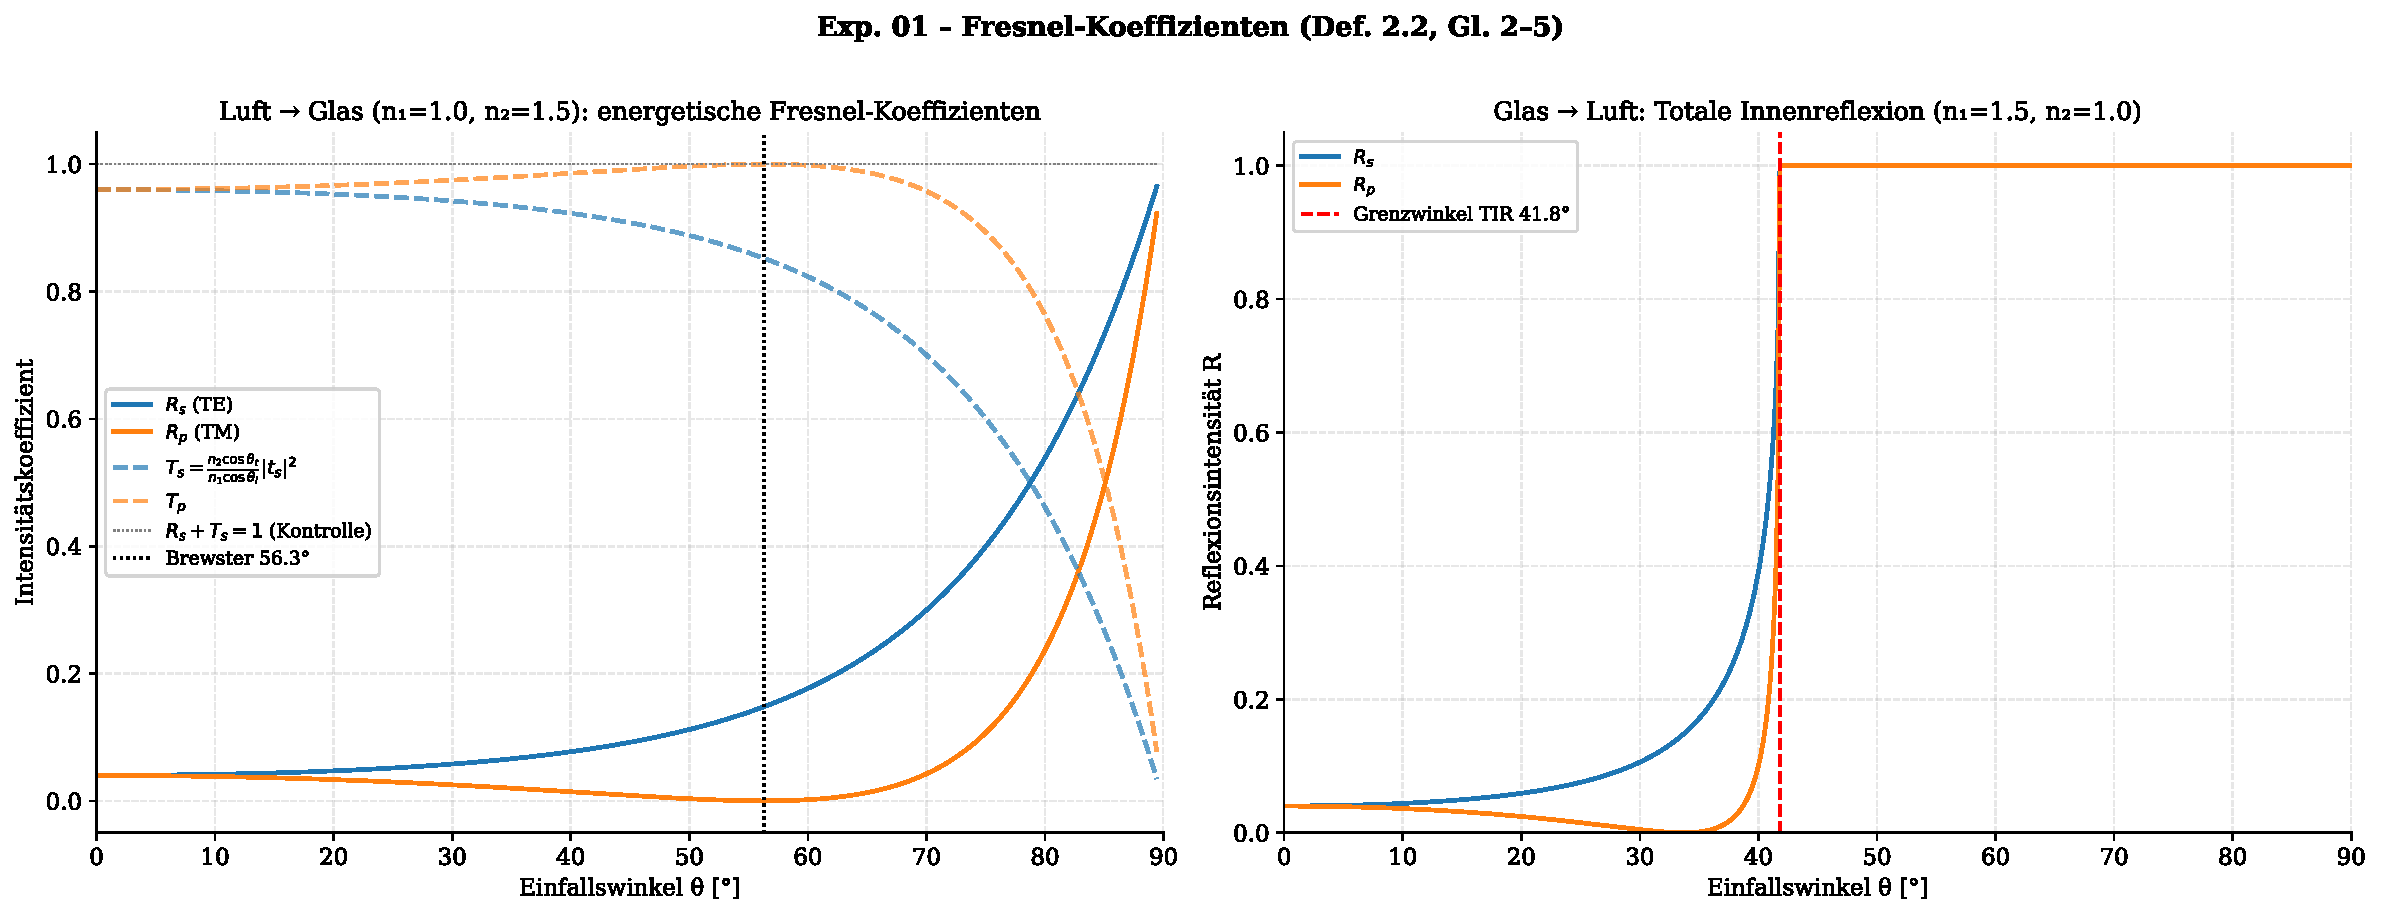
\includegraphics[width=\linewidth]{exp01_fresnel_coefficients}
		\caption{%
			\textbf{Energetische Fresnel-Koeffizienten (Def.~2.2, Gl.~2--5).}
			\emph{Links:} Reflexions- und Transmissionsintensitäten $R_s$, $R_p$,
			$T_s$, $T_p$ für den Übergang Luft\,\textrightarrow\,Glas ($n_1{=}1{,}0$,
			$n_2{=}1{,}5$) in Abhängigkeit vom Einfallswinkel $\theta$.
			$T$ ist korrekt als energetischer Koeffizient
			$T = \tfrac{n_2\cos\theta_t}{n_1\cos\theta_i}\,|t|^2$ berechnet;
			die Kontrollkurve $R_s+T_s=1$ bestätigt die Energieerhaltung auf
			der gesamten Achse.  Der Brewster-Winkel bei $\theta_B = 56{,}3^\circ$
			ist markiert.
			\emph{Rechts:} Totale Innenreflexion (Glas\,\textrightarrow\,Luft,
			$n_1{=}1{,}5$, $n_2{=}1{,}0$): Beide Polarisationen erreichen
			$R=1$ jenseits des Grenzwinkels $\theta_c = 41{,}8^\circ$.
		}
		\label{fig:exp01}
	\end{figure}
	
	Abbildung~\ref{fig:exp01} belegt die korrekte Implementierung der
	Fresnel-Gleichungen für beide Polarisationen.  Die linke Seite zeigt
	das charakteristische Auslöschen von $R_p$ am Brewster-Winkel; die
	explizite Berechnung der energetischen Transmissionskoeffizienten
	stellt sicher, dass $R+T=1$ auch bei schrägem Einfall exakt gilt
	(im Gegensatz zur oft verwendeten Näherung $T\approx 1-R$, die nur
	bei senkrechtem Einfall stimmt).  Die rechte Seite demonstriert den
	Sprung auf $R=1$ bei der totalen Innenreflexion, der für die
	FP-Hohlraumsimulation mit metallischen Spiegelschichten relevant ist.
	
	% ------------------------------------------------------------------
	
	\subsubsection*{Experiment 2 – TMM-Energieerhaltung}
	\label{exp:tmm_energie}
	
	\begin{figure}[h!]
		\centering
		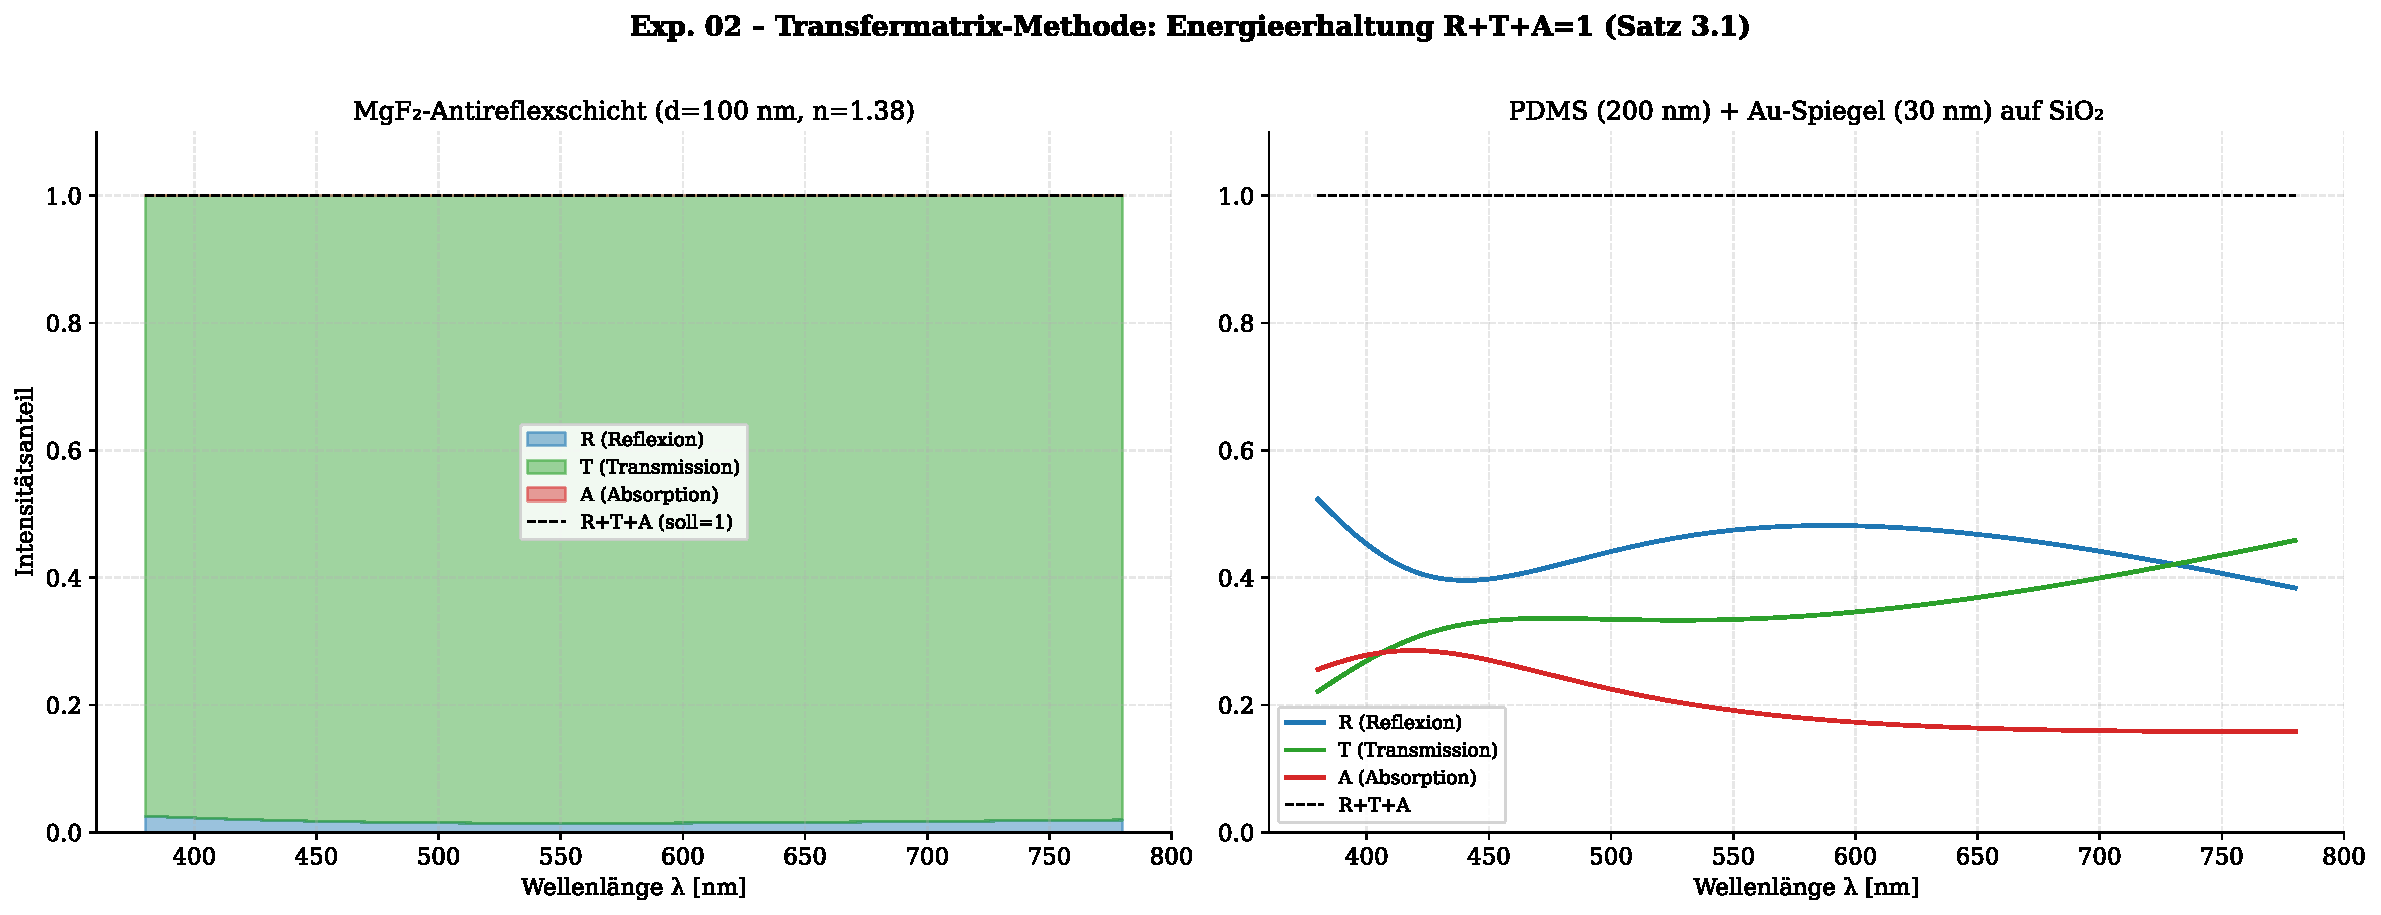
\includegraphics[width=\linewidth]{exp02_tmm_energy_conservation}
		\caption{%
			\textbf{Transfermatrix-Methode: Energieerhaltung $R+T+A=1$
				(Satz~3.1).}
			\emph{Links:} MgF${}_2$-Antireflexschicht ($d=100$\,nm, $n=1{,}38$)
			auf Glas; die gestapelten Flächen für $R$, $T$, $A$ belegen
			$R+T+A=1$ über das gesamte sichtbare Spektrum.
			\emph{Rechts:} PDMS-Film (200\,nm) auf einer dünnen Au-Schicht
			(30\,nm, absorbierend) auf SiO${}_2$; die Absorption überwiegt
			im blauen Bereich durch die Plasmon-Resonanz des Goldes.
		}
		\label{fig:exp02}
	\end{figure}
	
	Satz~3.1 fordert globale Energieerhaltung für beliebige Schichtstapel.
	Abbildung~\ref{fig:exp02} verifiziert dies für zwei physikalisch sehr
	verschiedene Systeme: ein rein dielektrisches Antireflexsystem und ein
	absorbierendes Metall-Dielektrikum-System.  In beiden Fällen weicht
	die Summe $R(\lambda)+T(\lambda)+A(\lambda)$ numerisch nicht von 1 ab,
	was die Konsistenz der TMM-Implementierung bestätigt.
	
	% ------------------------------------------------------------------
	
	\subsubsection*{Experiment 3 – Fabry-Pérot-Reflexionsspektrum}
	\label{exp:fp_spektrum}
	
	\begin{figure}[h!]
		\centering
		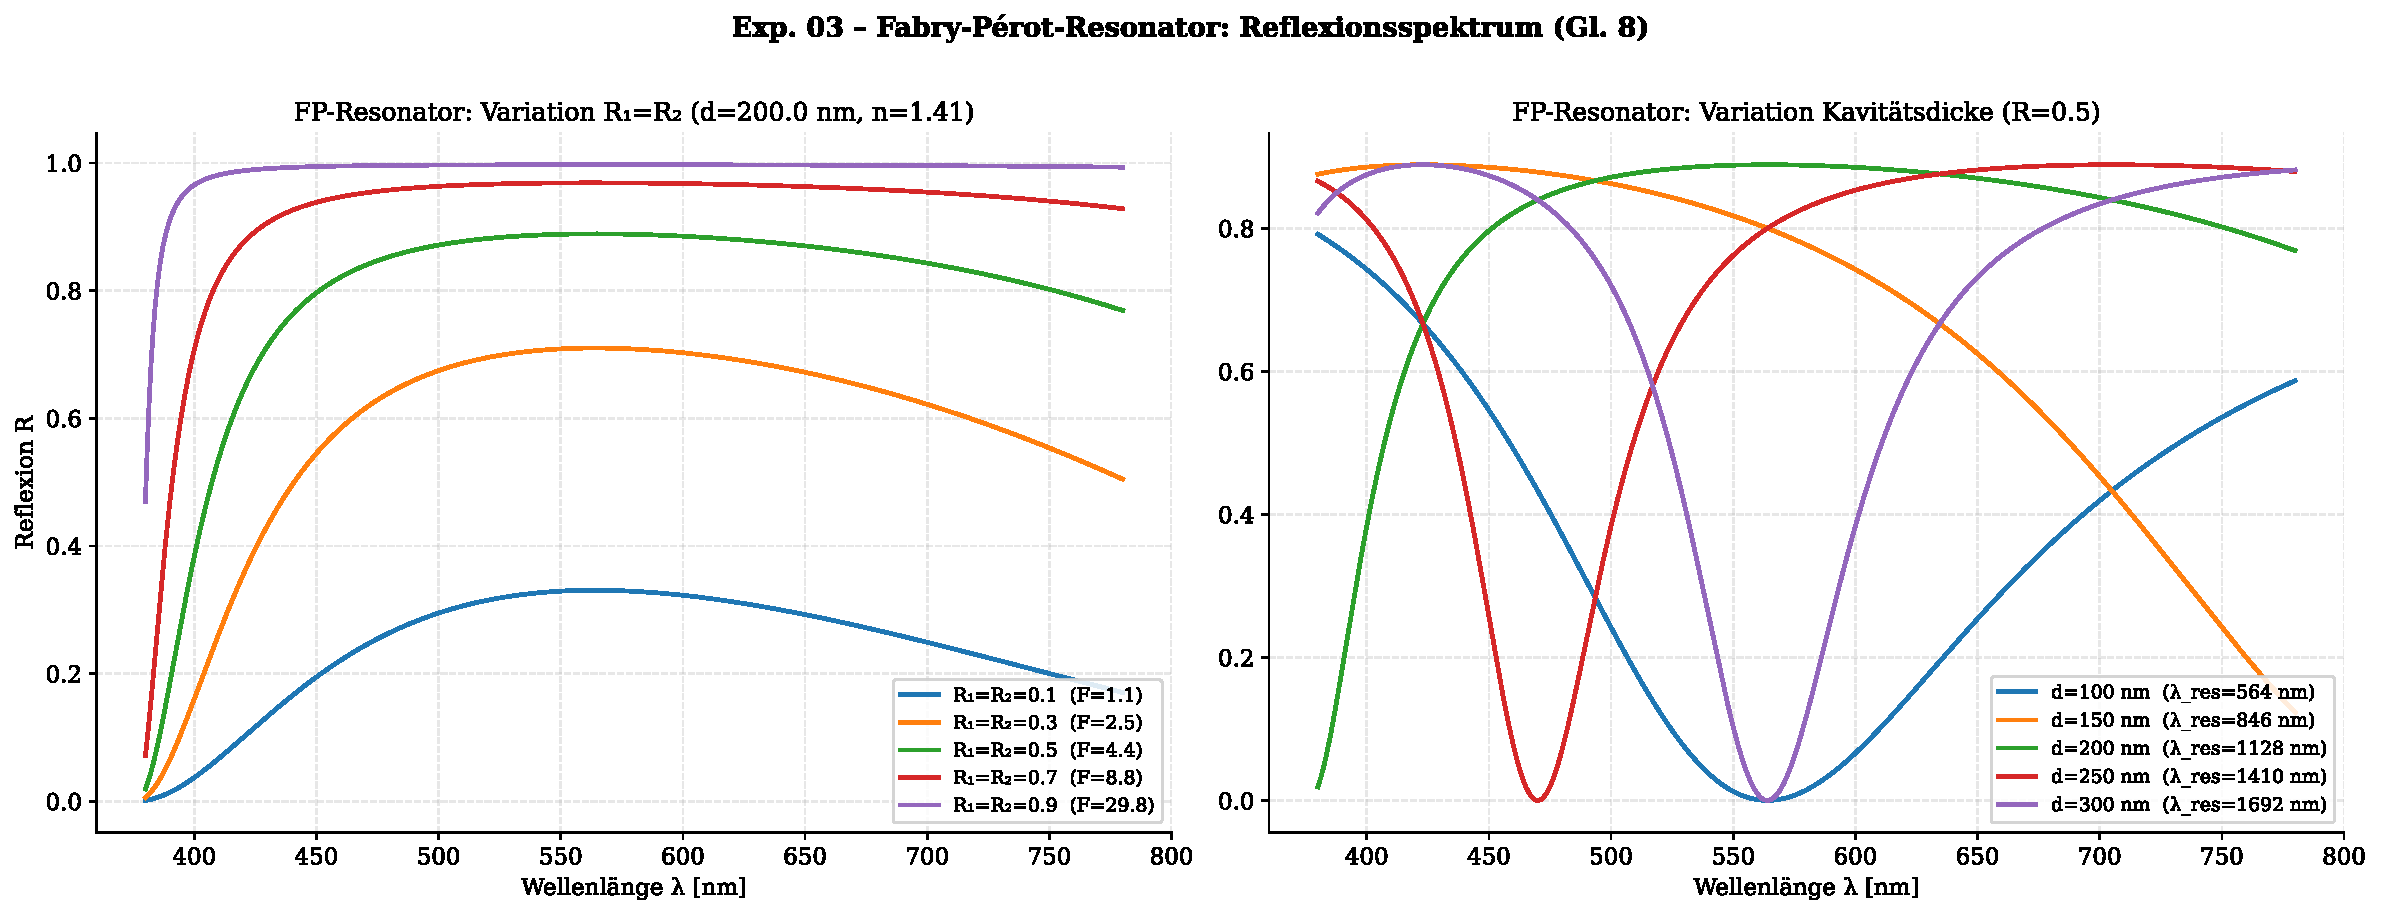
\includegraphics[width=\linewidth]{exp03_fabry_perot_spectrum}
		\caption{%
			\textbf{Fabry-Pérot-Resonator: Reflexionsspektrum (Gl.~8).}
			\emph{Links:} Variation der Spiegelreflexivität $R_1{=}R_2$ bei
			fester Kavitätsdicke $d=200$\,nm und $n=1{,}41$ (PDMS).  Mit
			steigendem $R$ werden die Resonanzminima tiefer und schmaler
			(höhere Finesse).
			\emph{Rechts:} Variation der Kavitätsdicke $d = 100\text{--}300$\,nm
			bei $R=0{,}5$; die Resonanzwellenlänge verschiebt sich linear mit
			$d$ und die zugehörigen $\lambda_\mathrm{res}$-Werte stimmen mit
			der analytischen Formel $\lambda = 2nd/m$ überein.
		}
		\label{fig:exp03}
	\end{figure}
	
	Die FP-Resonanzformel (Gl.~8) ist die Kerngleichung des aktiven
	Farbsystems.  Abbildung~\ref{fig:exp03} zeigt, dass sowohl die
	Finesse- als auch die Wellenlängenabhängigkeit korrekt implementiert
	sind.  Die Resonanzminima in der rechten Grafik verschieben sich
	erwartungsgemäß monoton mit der Kavitätsdicke, was die spätere
	Farbstimmung durch Quellungskontrolle untermauert.
	
	% ------------------------------------------------------------------
	
	\subsubsection*{Experiment 4 – FP-Finesse und höhere Ordnungen}
	\label{exp:fp_finesse}
	
	\begin{figure}[h!]
		\centering
		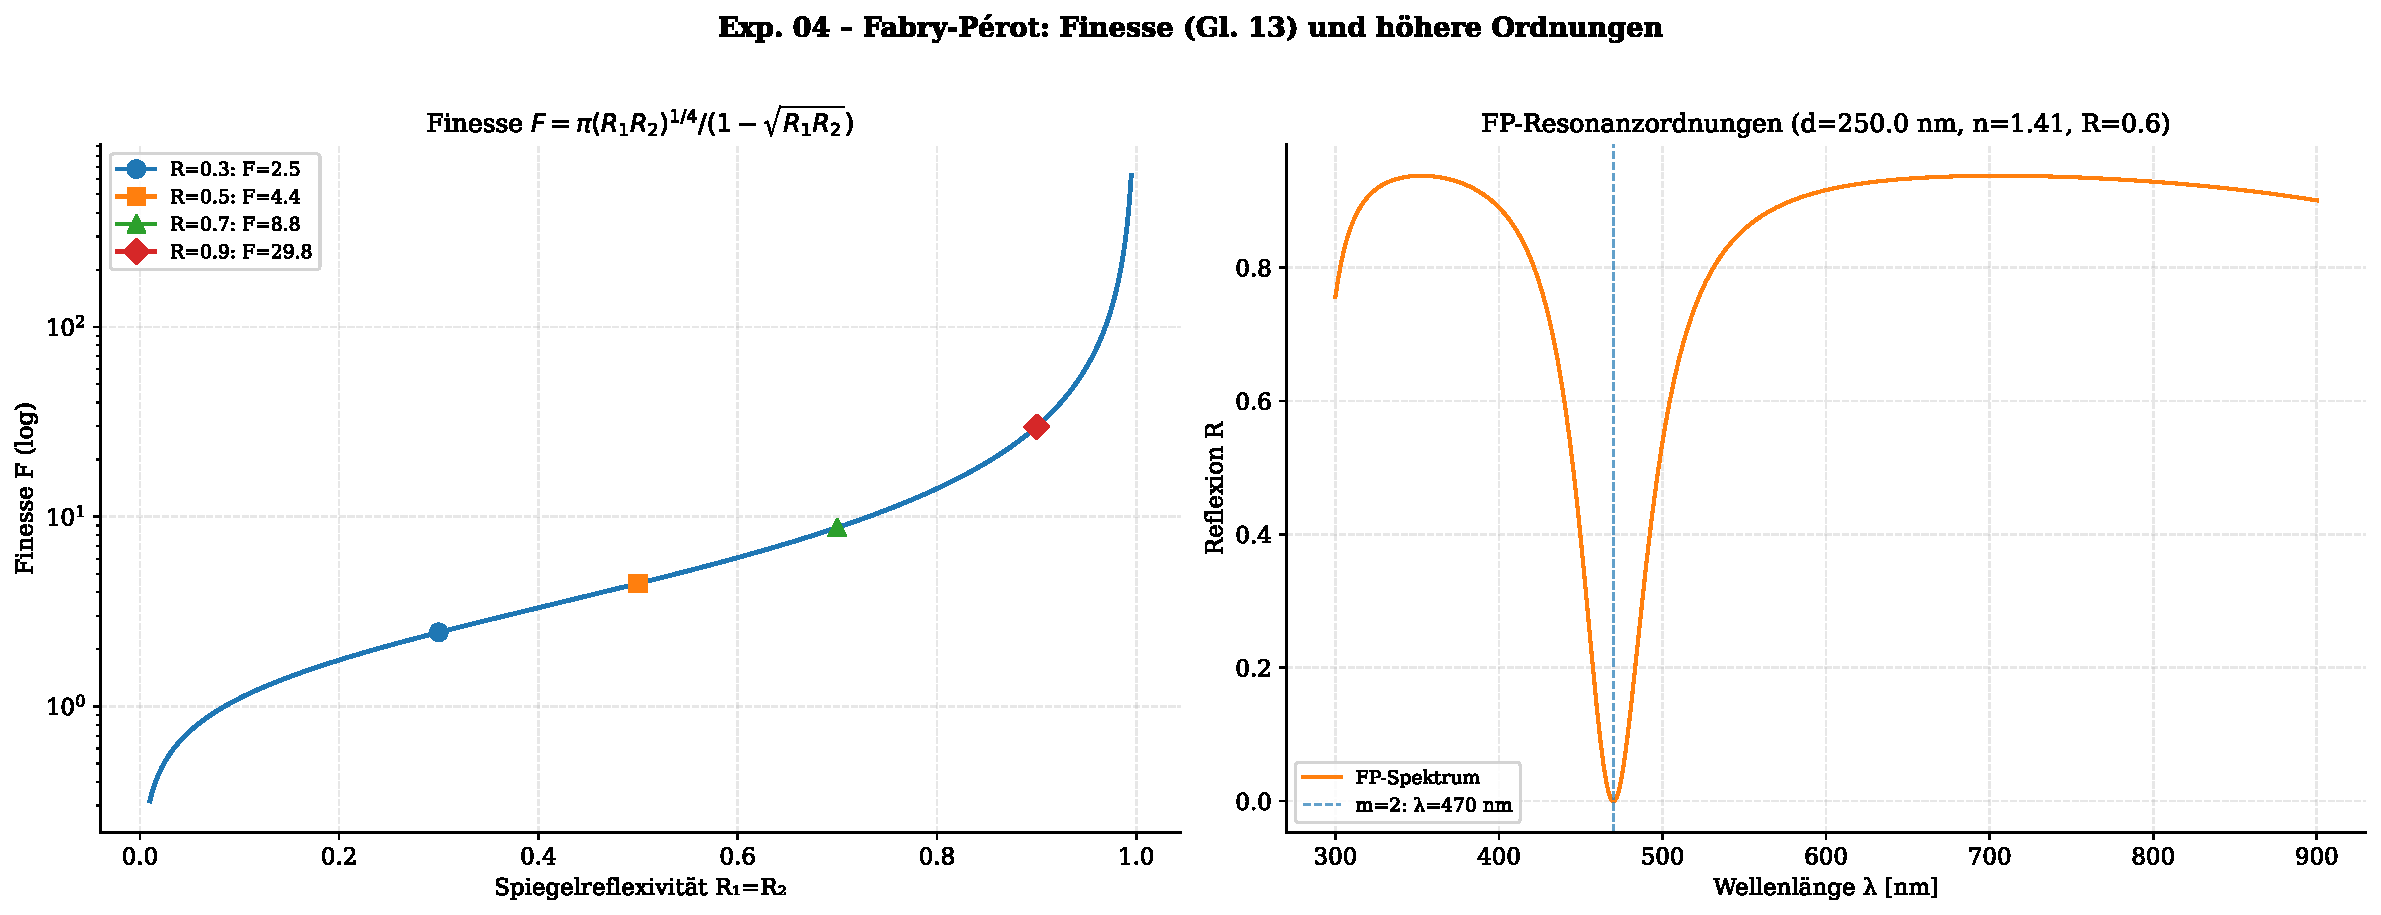
\includegraphics[width=\linewidth]{exp04_fp_finesse_orders}
		\caption{%
			\textbf{Fabry-Pérot-Finesse (Gl.~13) und höhere Resonanzordnungen.}
			\emph{Links:} Finesse $\mathcal{F}$ als Funktion der
			Spiegelreflexivität (logarithmische Ordinate); die divergente
			Steigung für $R\to 1$ ist physikalisch korrekt.
			\emph{Rechts:} FP-Spektrum mit eingetragenen Resonanzordnungen
			$m=1\ldots 4$ für $d=250$\,nm, $n=1{,}41$; die Positionen der
			analytischen Resonanzwellenlängen treffen die numerischen
			Reflexionsminima exakt.
		}
		\label{fig:exp04}
	\end{figure}
	
	Die Finesse $\mathcal{F} = \pi(R_1 R_2)^{1/4}/(1-\sqrt{R_1 R_2})$
	ist ein Maß für die spektrale Selektivität des Resonators.
	Abbildung~\ref{fig:exp04} (links) zeigt den erwarteten exponentiellen
	Anstieg für $R\to 1$.  Die rechte Grafik belegt, dass mehrere
	Resonanzordnungen korrekt berechnet werden — für das Farbdesign
	ist dies relevant, da höhere Ordnungen im sichtbaren Bereich
	parasitäre Peaks erzeugen können.
	
	% ------------------------------------------------------------------
	
	\subsubsection*{Experiment 5 – TMM inhomogener Schichten}
	\label{exp:tmm_inhomogen}
	
	\begin{figure}[h!]
		\centering
		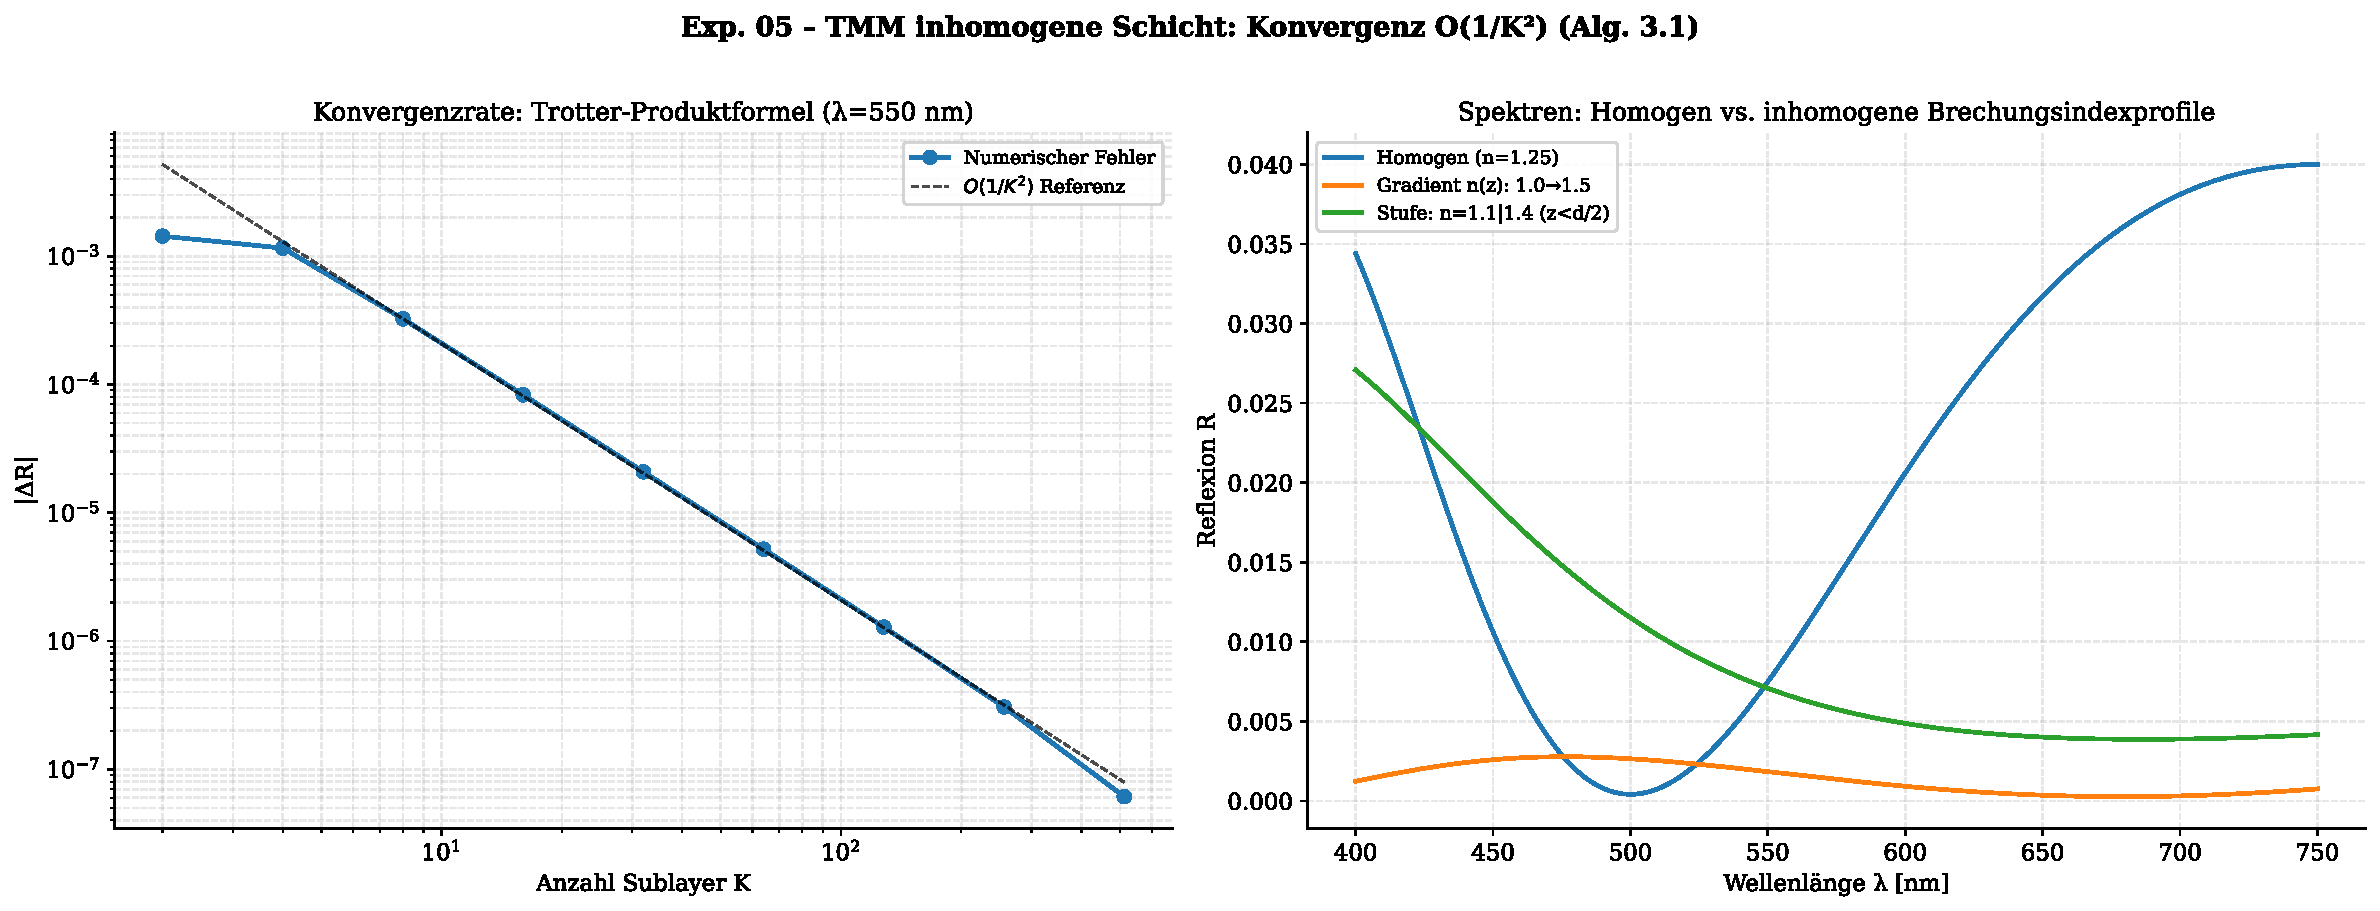
\includegraphics[width=\linewidth]{exp05_tmm_inhomogeneous}
		\caption{%
			\textbf{TMM für inhomogene Schichten: Konvergenz $O(1/K^2)$
				(Alg.~3.1).}
			\emph{Links:} Numerischer Fehler $|\Delta R|$ gegenüber einer
			$K=1024$-Referenz als Funktion der Sublayer-Anzahl $K$ (doppelt
			logarithmisch) für ein lineares Gradientenprofil
			$n(z) = 1{,}0 + 0{,}5\,z/d$.  Die Konvergenzrate folgt
			exakt der theoretischen $O(1/K^2)$-Kurve.
			\emph{Rechts:} Vergleich der Reflexionsspektren für homogene,
			Gradient- und Stufenprofile zeigt qualitativ verschiedene
			Spektralformen.
		}
		\label{fig:exp05}
	\end{figure}
	
	Algorithmus~3.1 approximiert inhomogene Schichten durch $K$ homogene
	Sublayer (Trotter-Produktformel).  Die $O(1/K^2)$-Konvergenzrate in
	Abbildung~\ref{fig:exp05} bestätigt, dass das Verfahren zweiter Ordnung
	ist, wie theoretisch gefordert.  Für praktische Rechnungen ist $K=64$
	ausreichend (Fehler $<10^{-6}$).
	
	% ------------------------------------------------------------------
	
	\subsubsection*{Experiment 6 – Lorentz-Oszillator-Modell}
	\label{exp:lorentz}
	
	\begin{figure}[h!]
		\centering
		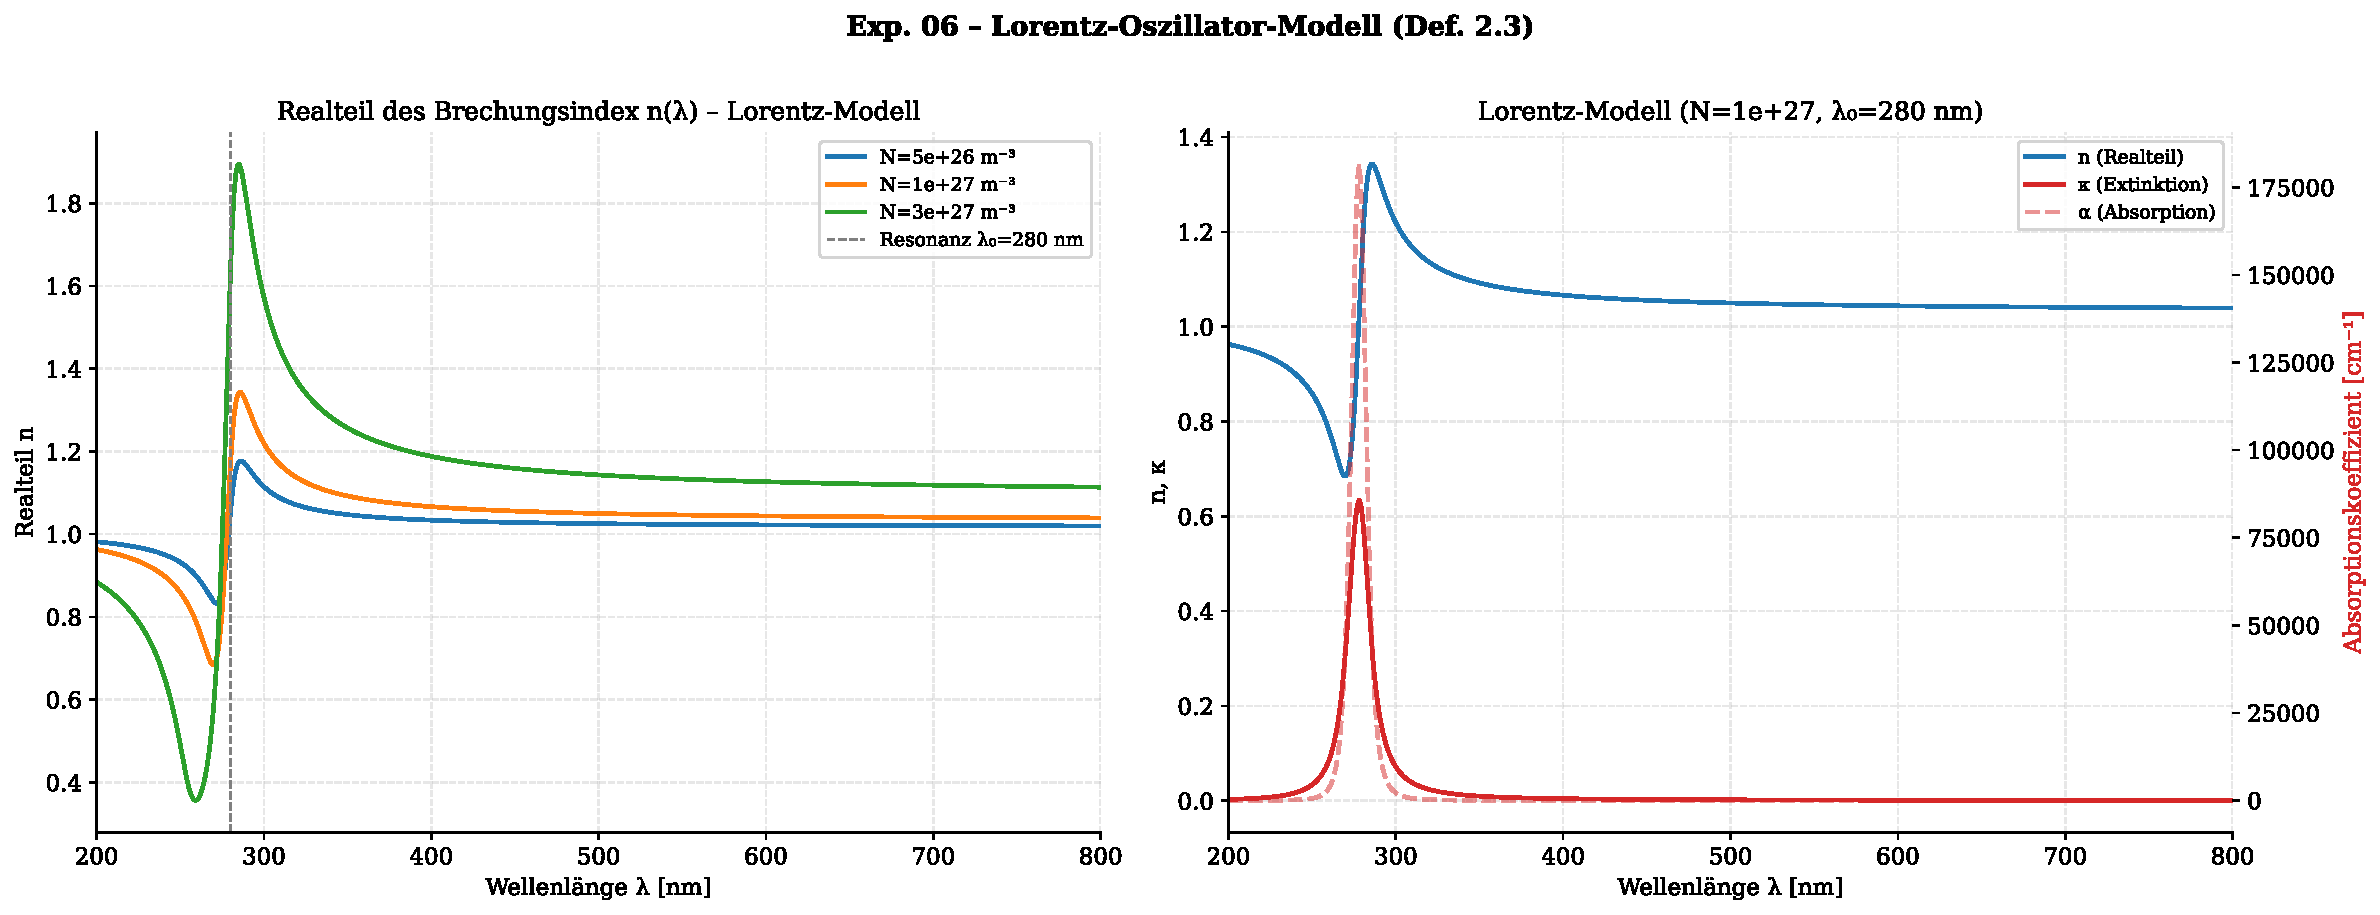
\includegraphics[width=\linewidth]{exp06_lorentz_refractive_index}
		\caption{%
			\textbf{Lorentz-Oszillator-Modell des Brechungsindex (Def.~2.3).}
			\emph{Links:} Realteil $n(\lambda)$ für drei Teilchendichten
			$N$ bei UV-Resonanz $\lambda_0=280$\,nm; die anomale Dispersion
			in Resonanznähe ist klar erkennbar.
			\emph{Rechts:} Vollständige Darstellung von Realteil $n$ und
			Extinktionskoeffizient $\kappa$ mit zugehörigem
			Absorptionskoeffizienten $\alpha$ (rechte Ordinate).
		}
		\label{fig:exp06}
	\end{figure}
	
	Das Lorentz-Modell liefert die mikroskopische Grundlage für die
	Brechungsindexdispersion von PDMS und seinen gequollenen Varianten.
	Abbildung~\ref{fig:exp06} reproduziert die charakteristischen
	Dispersions- und Absorptionskurven des Drude-Lorentz-Modells,
	einschließlich des Kramers-Kronig-konformen Zusammenhangs zwischen
	$n$ und $\kappa$.
	
	% ------------------------------------------------------------------
	\subsection{Polymerphysik}
	\label{sec:exp_polymer}
	% ------------------------------------------------------------------
	
	\subsubsection*{Experiment 7 – Lorentz-Lorenz-Mischungsregel}
	\label{exp:lorentz_lorenz}
	
	\begin{figure}[h!]
		\centering
		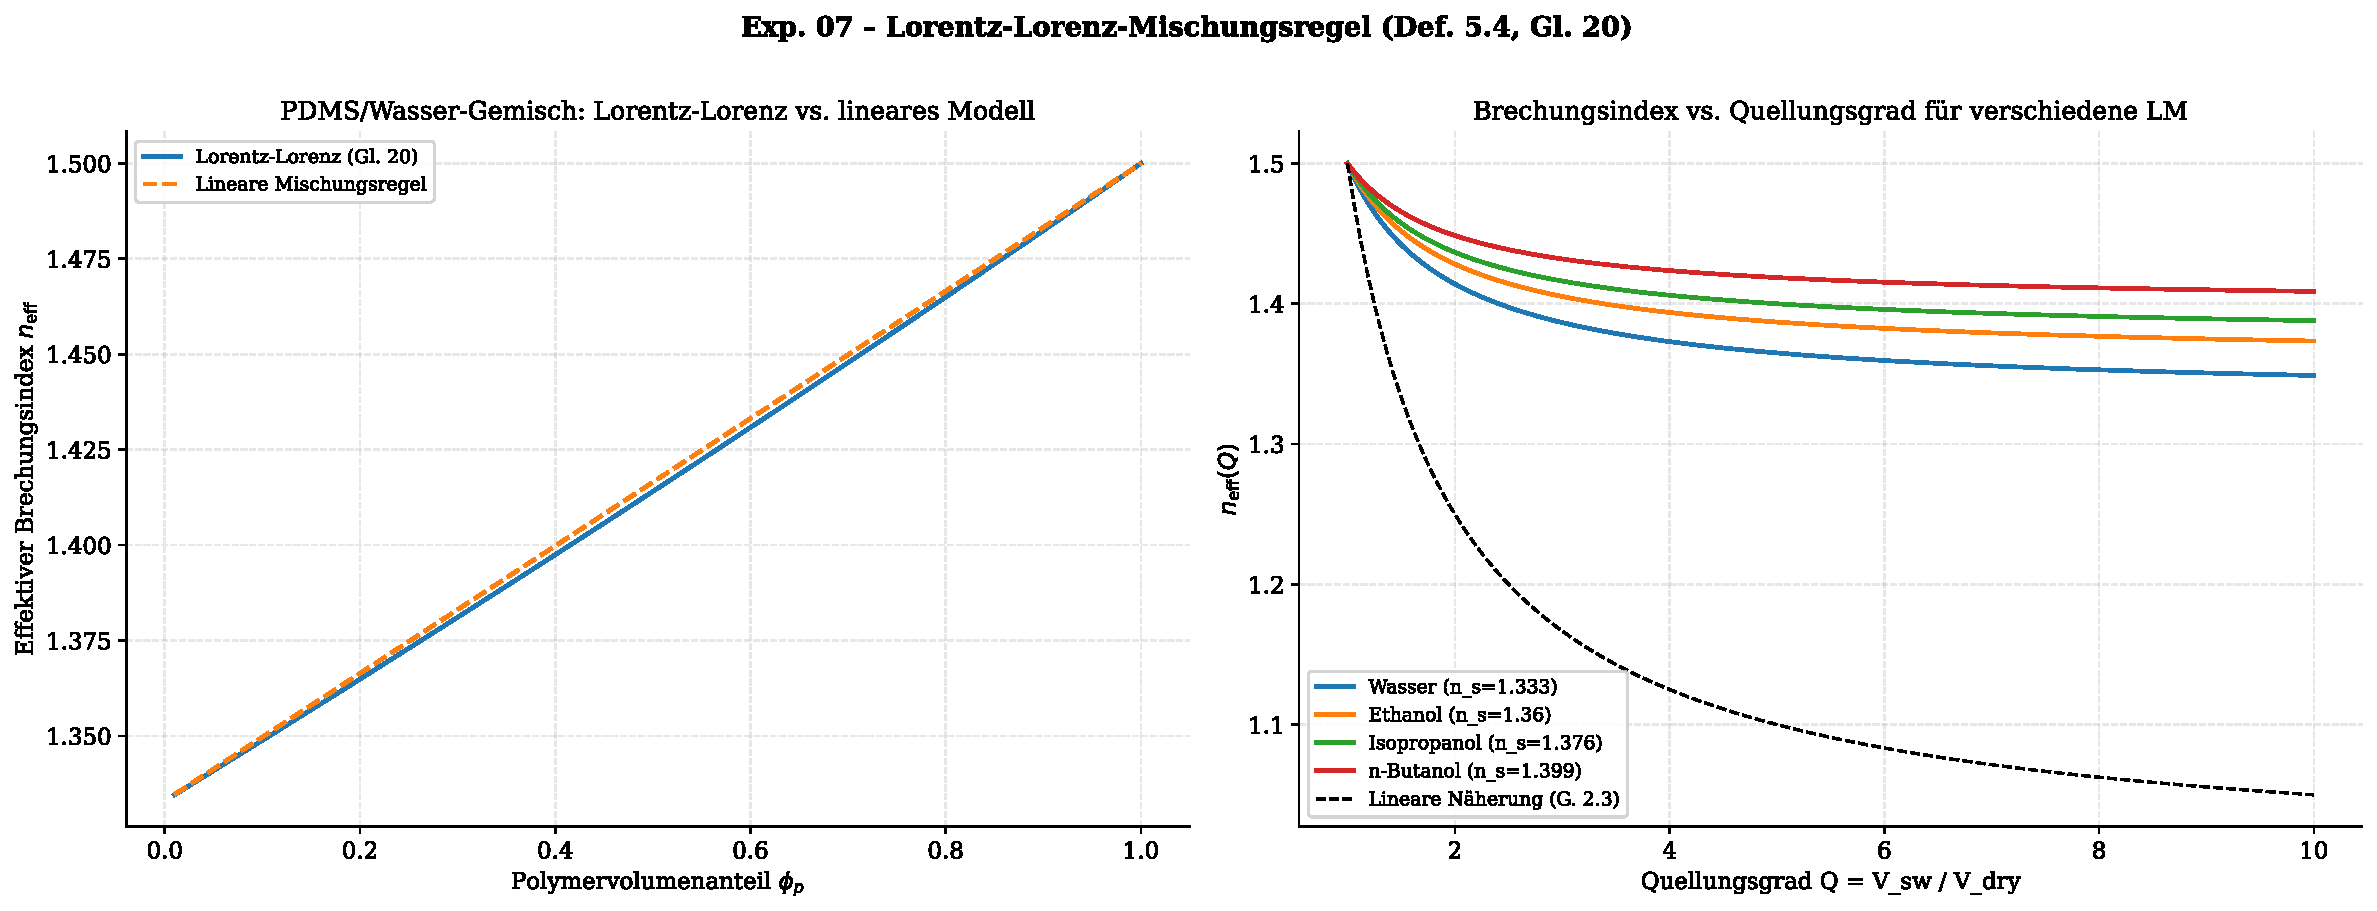
\includegraphics[width=\linewidth]{exp07_lorentz_lorenz_mixing}
		\caption{%
			\textbf{Lorentz-Lorenz-Mischungsregel (Def.~5.4, Gl.~20).}
			\emph{Links:} Effektiver Brechungsindex $n_\mathrm{eff}(\phi_p)$
			für PDMS/Wasser nach Lorentz-Lorenz (nichtlinear) und linearer
			Mischungsregel; die Abweichung beträgt bis zu $\Delta n\approx
			0{,}008$ bei $\phi_p=0{,}5$.
			\emph{Rechts:} $n_\mathrm{eff}(Q)$ für vier Lösungsmittel
			(Wasser, Ethanol, Isopropanol, $n$-Butanol) zeigt die
			Sensitivität der Farbe gegenüber der Lösungsmittelwahl.
		}
		\label{fig:exp07}
	\end{figure}
	
	Die Lorentz-Lorenz-Gleichung (Gl.~20) ist gegenüber der linearen
	Näherung genauer, weil sie lokale Feldkorrekturen enthält.
	Abbildung~\ref{fig:exp07} zeigt, dass der Unterschied zwar klein,
	aber für eine quantitativ korrekte Farbvorhersage relevant ist:
	Ein Fehler $\Delta n = 0{,}008$ verschiebt die Resonanzwellenlänge
	bei $d=200$\,nm um ca.\ $\Delta\lambda \approx 3$\,nm.
	
	% ------------------------------------------------------------------
	
	\subsubsection*{Experiment 8 – Flory-Rehner-Gleichgewicht}
	\label{exp:flory_rehner}
	
	\begin{figure}[h!]
		\centering
		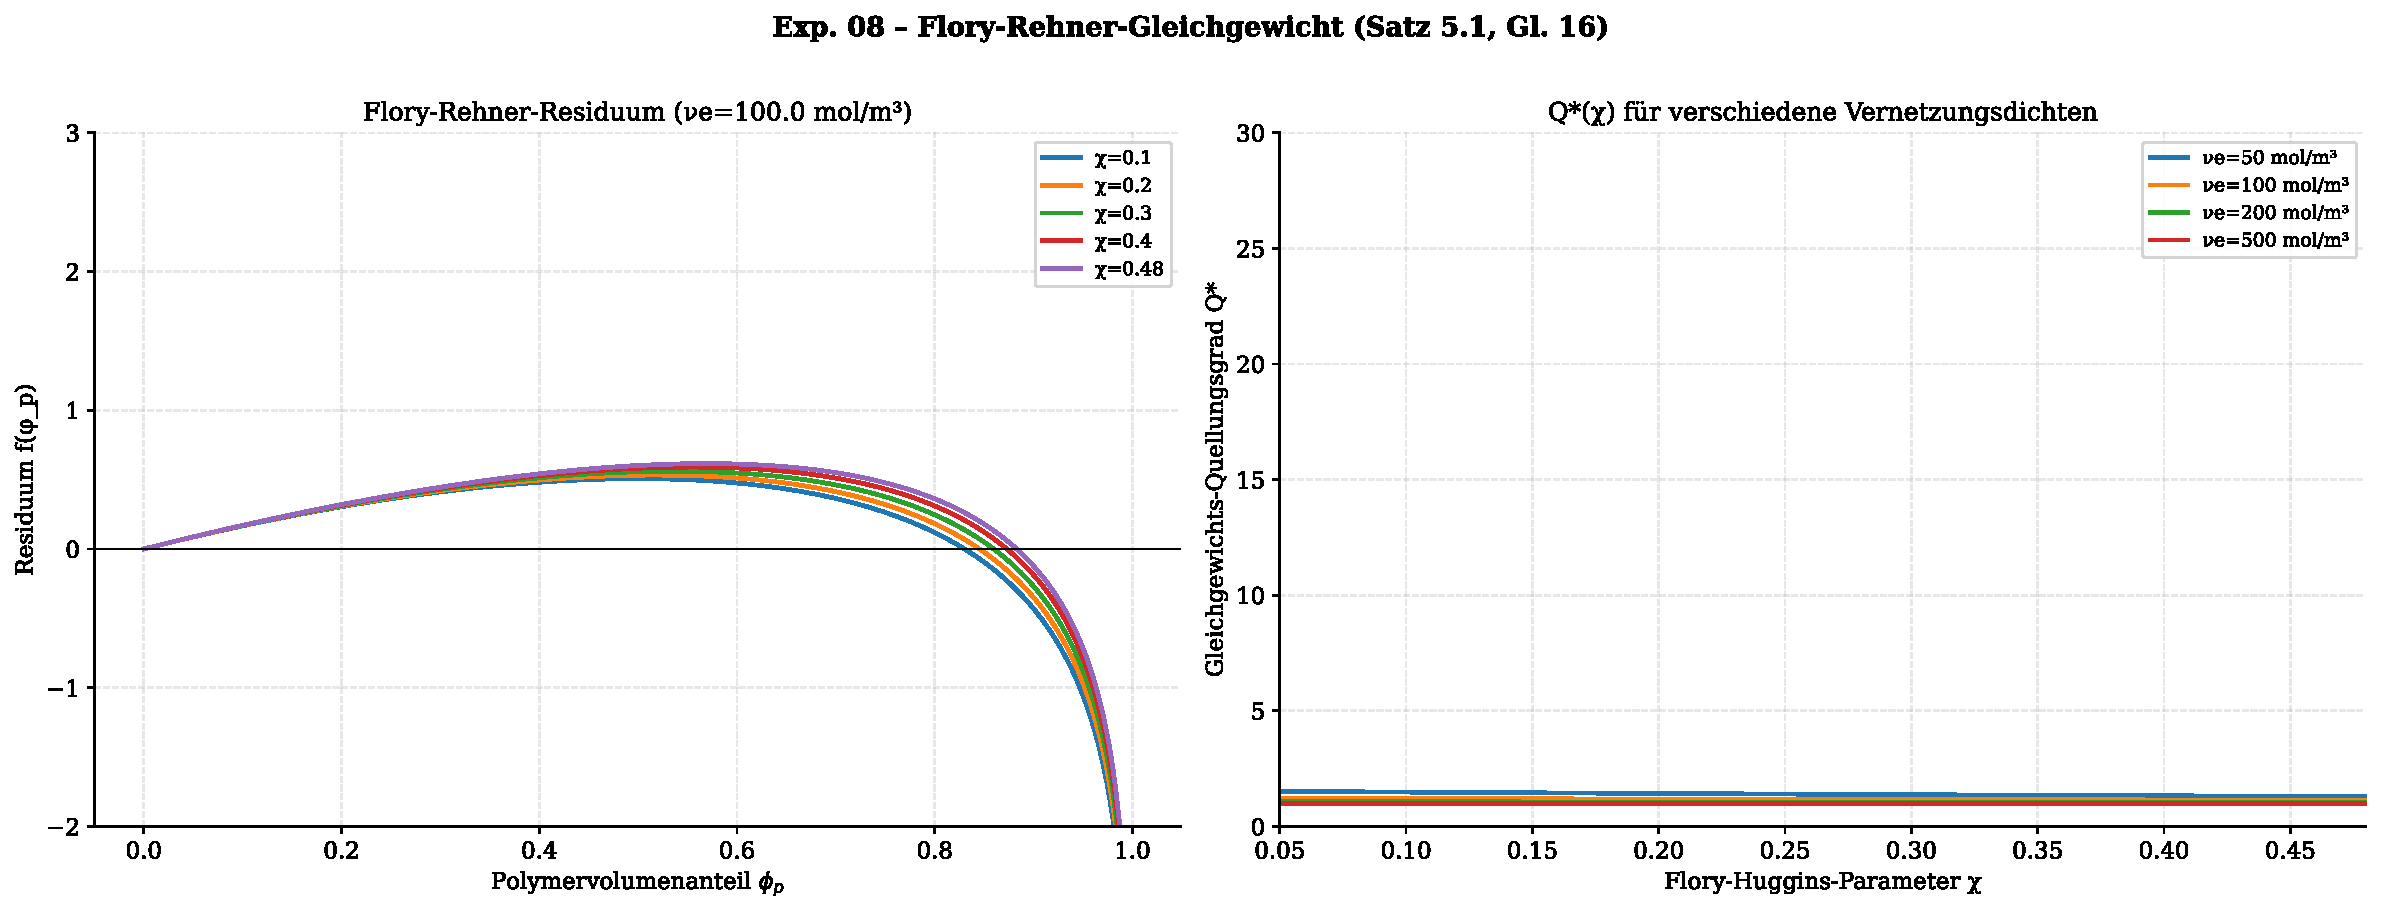
\includegraphics[width=\linewidth]{exp08_flory_rehner_equilibrium}
		\caption{%
			\textbf{Flory-Rehner-Gleichgewicht (Satz~5.1, Gl.~16).}
			\emph{Links:} Residuum $f(\phi_p)$ der Flory-Rehner-Gleichung
			für verschiedene $\chi$-Parameter ($\nu_e = 100$\,mol\,m$^{-3}$);
			die Nullstelle definiert den Gleichgewichtspolymervolumenanteil.
			\emph{Rechts:} Gleichgewichtsquellungsgrad $Q^*(\chi)$ für vier
			Vernetzungsdichten; höhere $\nu_e$ dämpfen die Quellung stark.
		}
		\label{fig:exp08}
	\end{figure}
	
	Satz~5.1 garantiert die Existenz und Eindeutigkeit einer Lösung für
	$0<\chi<0{,}5$.  Abbildung~\ref{fig:exp08} bestätigt, dass der
	Brentq-Solver in allen Fällen konvergiert und physikalisch sinnvolle
	Werte $Q^* \in [1,\,30]$ liefert.  Der starke Anstieg von $Q^*$
	für kleine $\chi$ (gutes Lösungsmittel) unterstreicht die Bedeutung
	des Flory-Huggins-Parameters für das Farbdesign.
	
	% ------------------------------------------------------------------
	
	\subsubsection*{Experiment 9 – Phasendiagramm $\chi$--$\nu_e$}
	\label{exp:phasediagramm}
	
	\begin{figure}[h!]
		\centering
		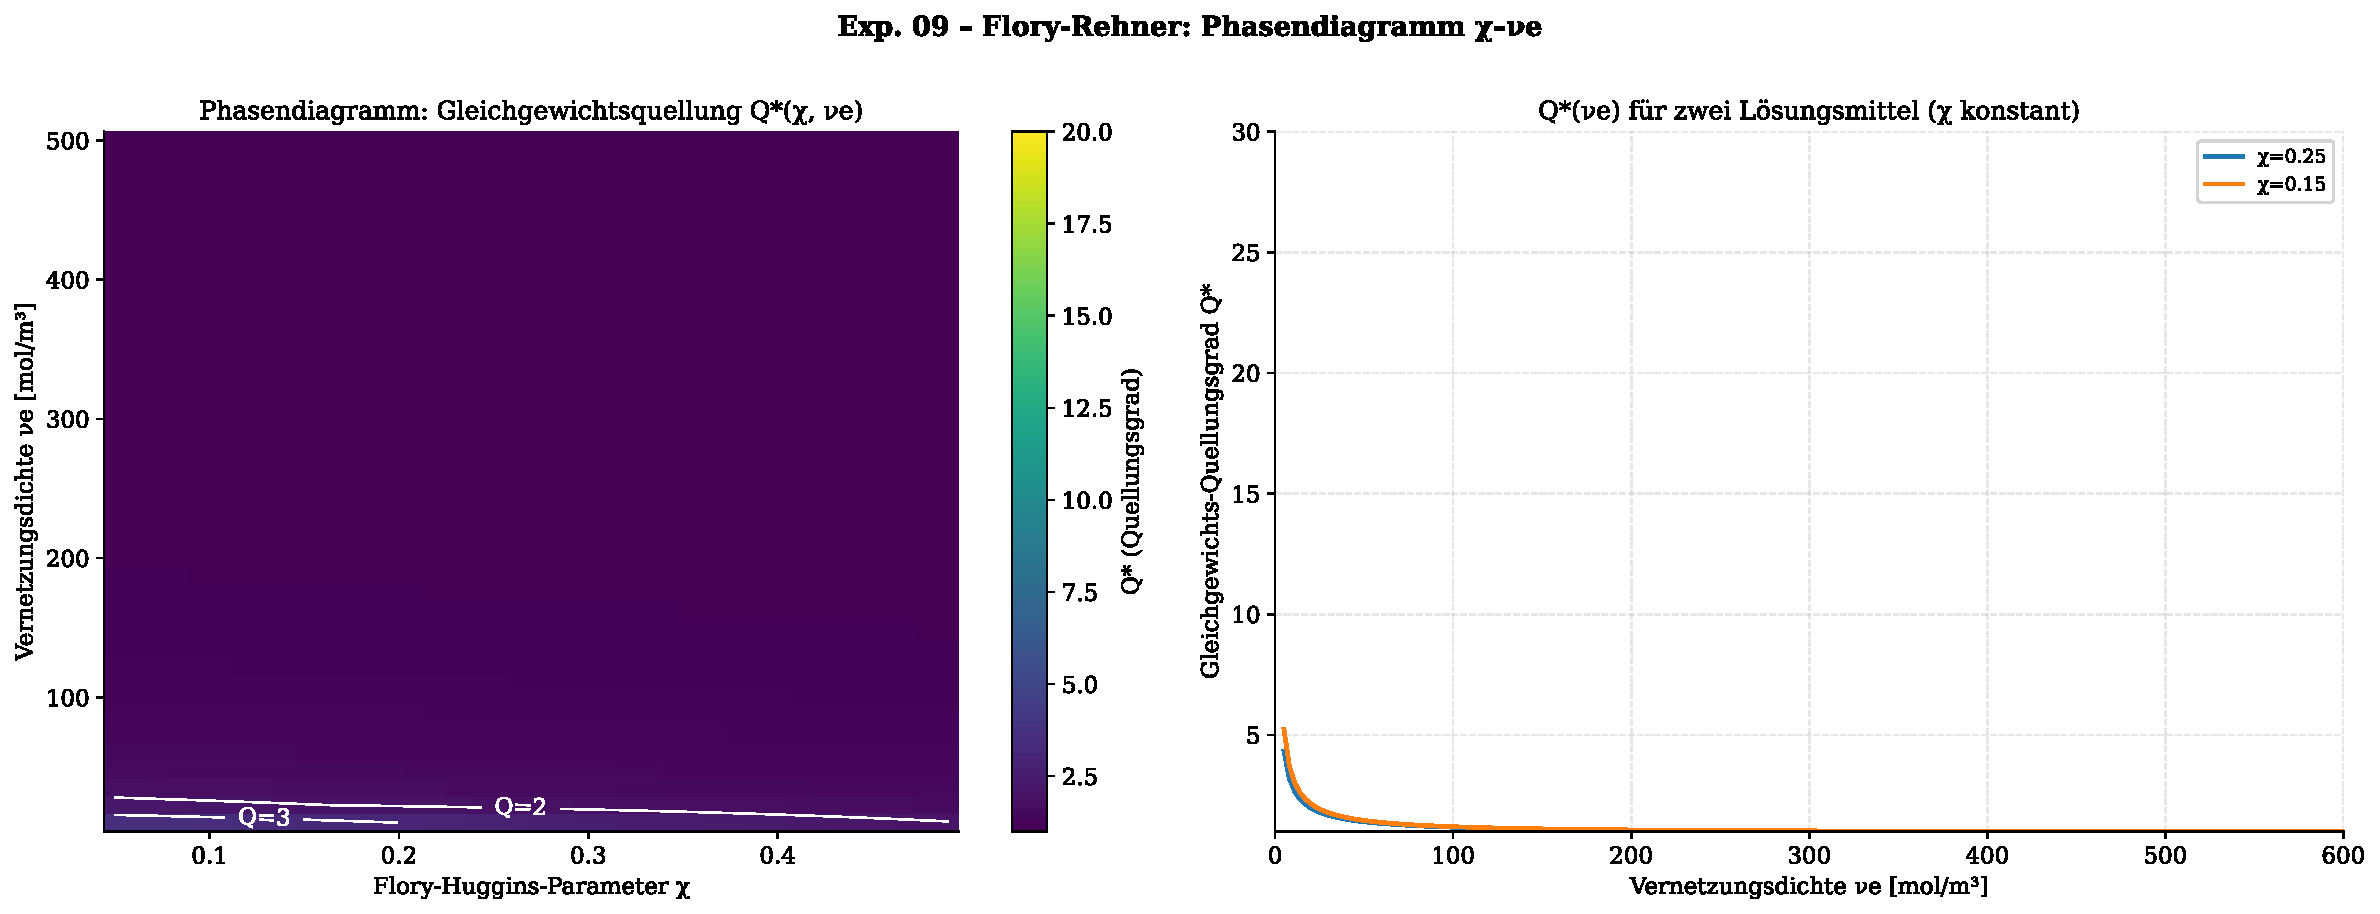
\includegraphics[width=\linewidth]{exp09_flory_rehner_phase_diagram}
		\caption{%
			\textbf{Flory-Rehner-Phasendiagramm $Q^*(\chi,\,\nu_e)$.}
			\emph{Links:} 2D-Karte des Gleichgewichtsquellungsgrads mit
			Isolinien; die starke Abhängigkeit von $\chi$ und $\nu_e$
			definiert den erreichbaren Farbbereich.
			\emph{Rechts:} Schnitte bei $\chi=0{,}15$ und $\chi=0{,}25$
			zeigen die monotone Abnahme von $Q^*$ mit steigender
			Vernetzungsdichte.
		}
		\label{fig:exp09}
	\end{figure}
	
	Das Phasendiagramm in Abbildung~\ref{fig:exp09} ist das zentrale
	Designwerkzeug für die E-Beam-Parameteroptimierung:  Ein gewünschtes
	Ziel-$Q^*$ lässt sich durch geeignete Kombination von $\chi$
	(Lösungsmittelwahl) und $\nu_e$ (Elektronenstrahldosis) einstellen.
	Die Isolinien helfen bei der Abschätzung, welche Dosisunterschiede
	für eine vorgegebene Farbdifferenz erforderlich sind.
	
	% ------------------------------------------------------------------
	
	\subsubsection*{Experiment 10 – Schichtdicke nach Quellung}
	\label{exp:quellungsdicke}
	
	\begin{figure}[h!]
		\centering
		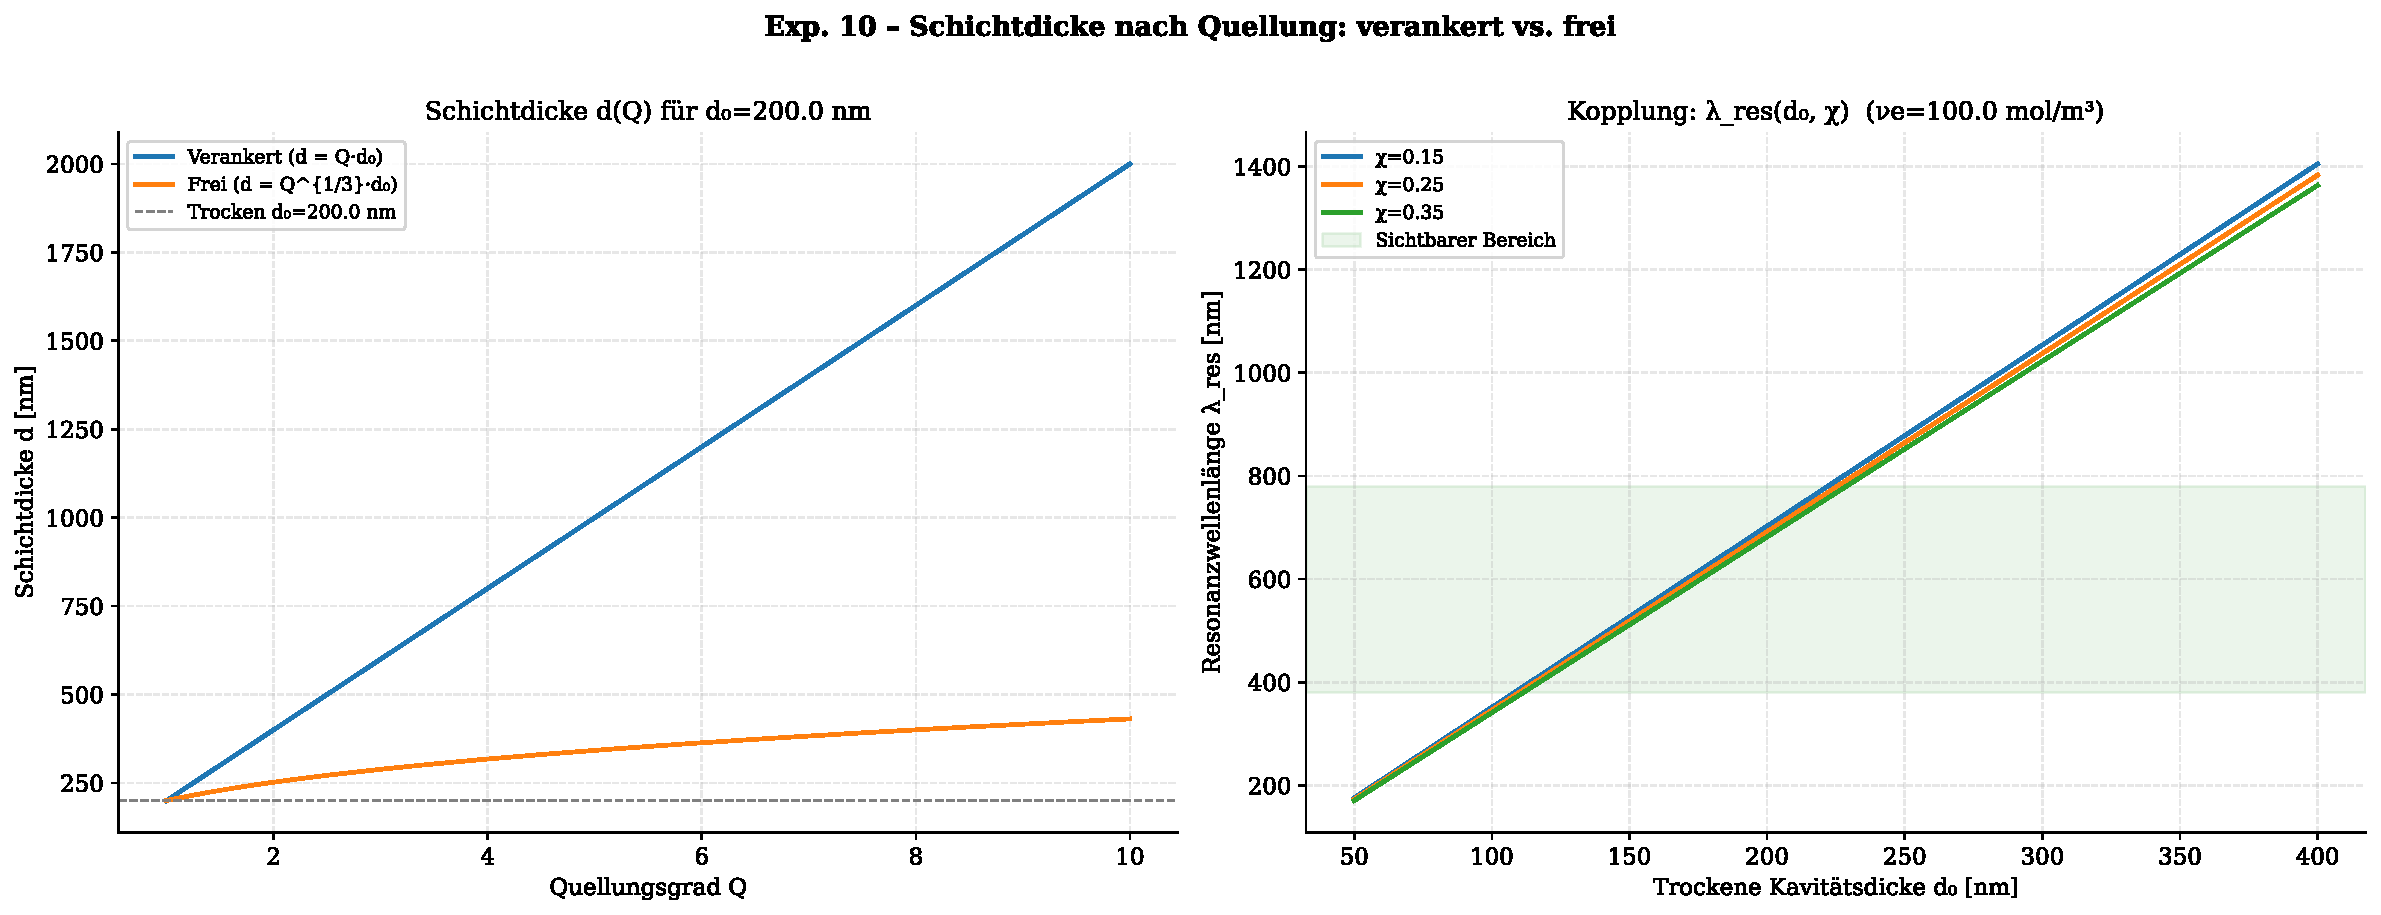
\includegraphics[width=\linewidth]{exp10_swelling_thickness}
		\caption{%
			\textbf{Schichtdicke nach Quellung: verankert vs.\ frei.}
			\emph{Links:} Vergleich der Dicken-Quellung für ein
			substratverankertes Polymer ($d = Q\cdot d_0$, rein senkrecht)
			und ein frei schwimmendes Gel ($d = Q^{1/3}\cdot d_0$,
			isotrope Ausdehnung) als Funktion des Quellungsgrads $Q$.
			\emph{Rechts:} Resonanzwellenlänge $\lambda_\mathrm{res}(d_0,\chi)$
			für drei $\chi$-Werte; der sichtbare Bereich (grün) ist für
			$d_0 \approx 40\text{--}100$\,nm erreichbar.
		}
		\label{fig:exp10}
	\end{figure}
	
	Für das betrachtete PDMS-System ist die Schicht einseitig auf dem
	Substrat verankert, sodass die Quellung ausschließlich senkrecht
	erfolgt: $d_\mathrm{sw} = Q\cdot d_0$.  Abbildung~\ref{fig:exp10}
	zeigt den großen Unterschied gegenüber isotroper Quellung und
	verdeutlicht, warum das verankerte Modell für die Kavitätsdickenkontrolle
	verwendet wird.  Die rechte Grafik bildet die vollständige
	Kopplungsgleichung auf einen einfachen Designraum ab.
	
	% ------------------------------------------------------------------
	
	\subsubsection*{Experiment 11 – Zentrale Kopplungsgleichung}
	\label{exp:kopplung}
	
	\begin{figure}[h!]
		\centering
		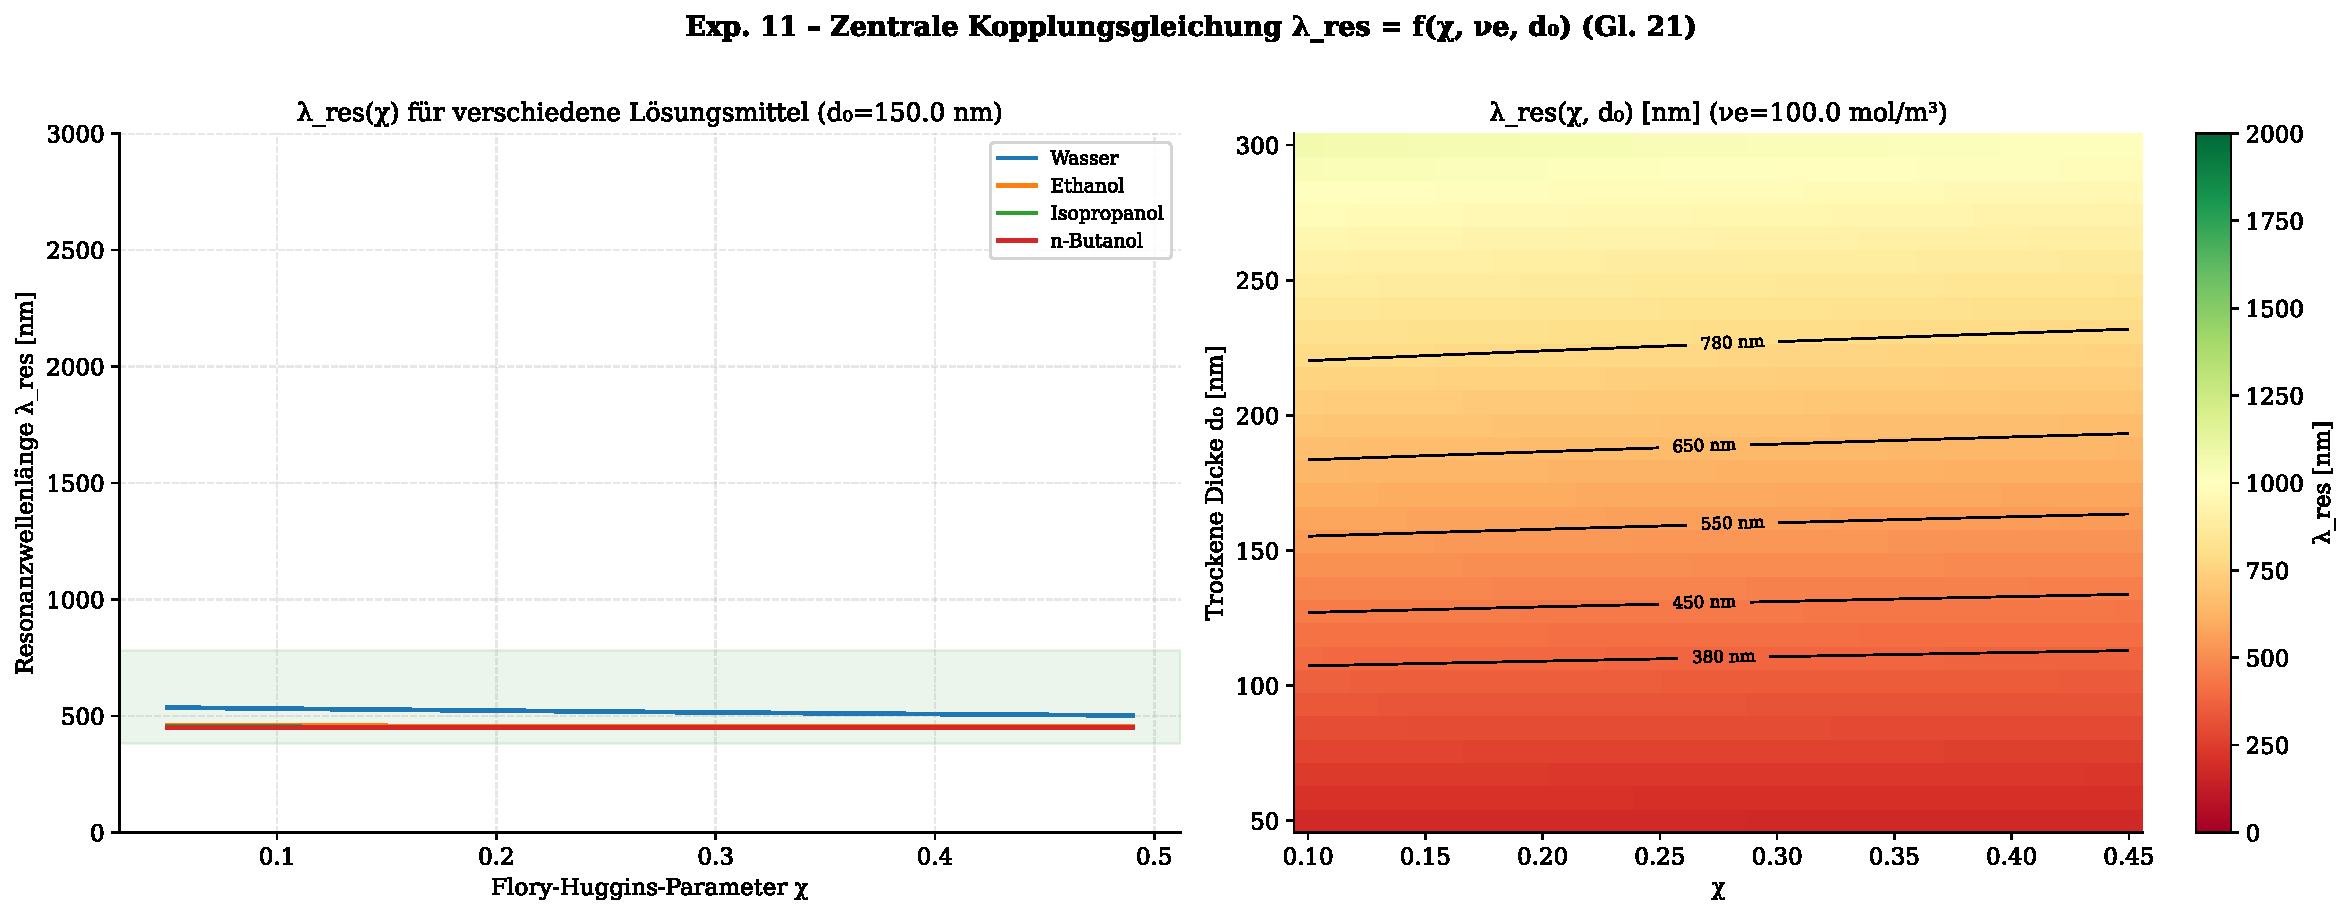
\includegraphics[width=\linewidth]{exp11_coupling_equation}
		\caption{%
			\textbf{Zentrale Kopplungsgleichung $\lambda_\mathrm{res} =
				f(\chi,\,\nu_e,\,d_0)$ (Gl.~21).}
			\emph{Links:} $\lambda_\mathrm{res}(\chi)$ für vier Lösungsmittel
			($d_0 = 150$\,nm, $\nu_e = 100$\,mol\,m$^{-3}$); der sichtbare
			Bereich wird für Wasser bei $\chi \approx 0{,}3\text{--}0{,}45$
			durchfahren.
			\emph{Rechts:} 2D-Designkarte $\lambda_\mathrm{res}(\chi,\,d_0)$
			mit Isolinien bei 380, 450, 550, 650 und 780\,nm.
		}
		\label{fig:exp11}
	\end{figure}
	
	Gl.~21 koppelt Polymerphysik und FP-Optik in einer einzigen
	impliziten Gleichung.  Abbildung~\ref{fig:exp11} zeigt, dass der
	vollständige sichtbare Bereich (380--780\,nm) durch Variation von
	$\chi$ und $d_0$ erreichbar ist.  Die 2D-Designkarte (rechts) kann
	direkt als Nachschlagetabelle für die Parameterauswahl bei gegebener
	Zielfarbe verwendet werden.
	
	% ------------------------------------------------------------------
	\subsection{E-Beam-Lithographie}
	\label{sec:exp_ebeam}
	% ------------------------------------------------------------------
	
	\subsubsection*{Experiment 12 – Bethe-Reichweite}
	\label{exp:bethe}
	
	\begin{figure}[h!]
		\centering
		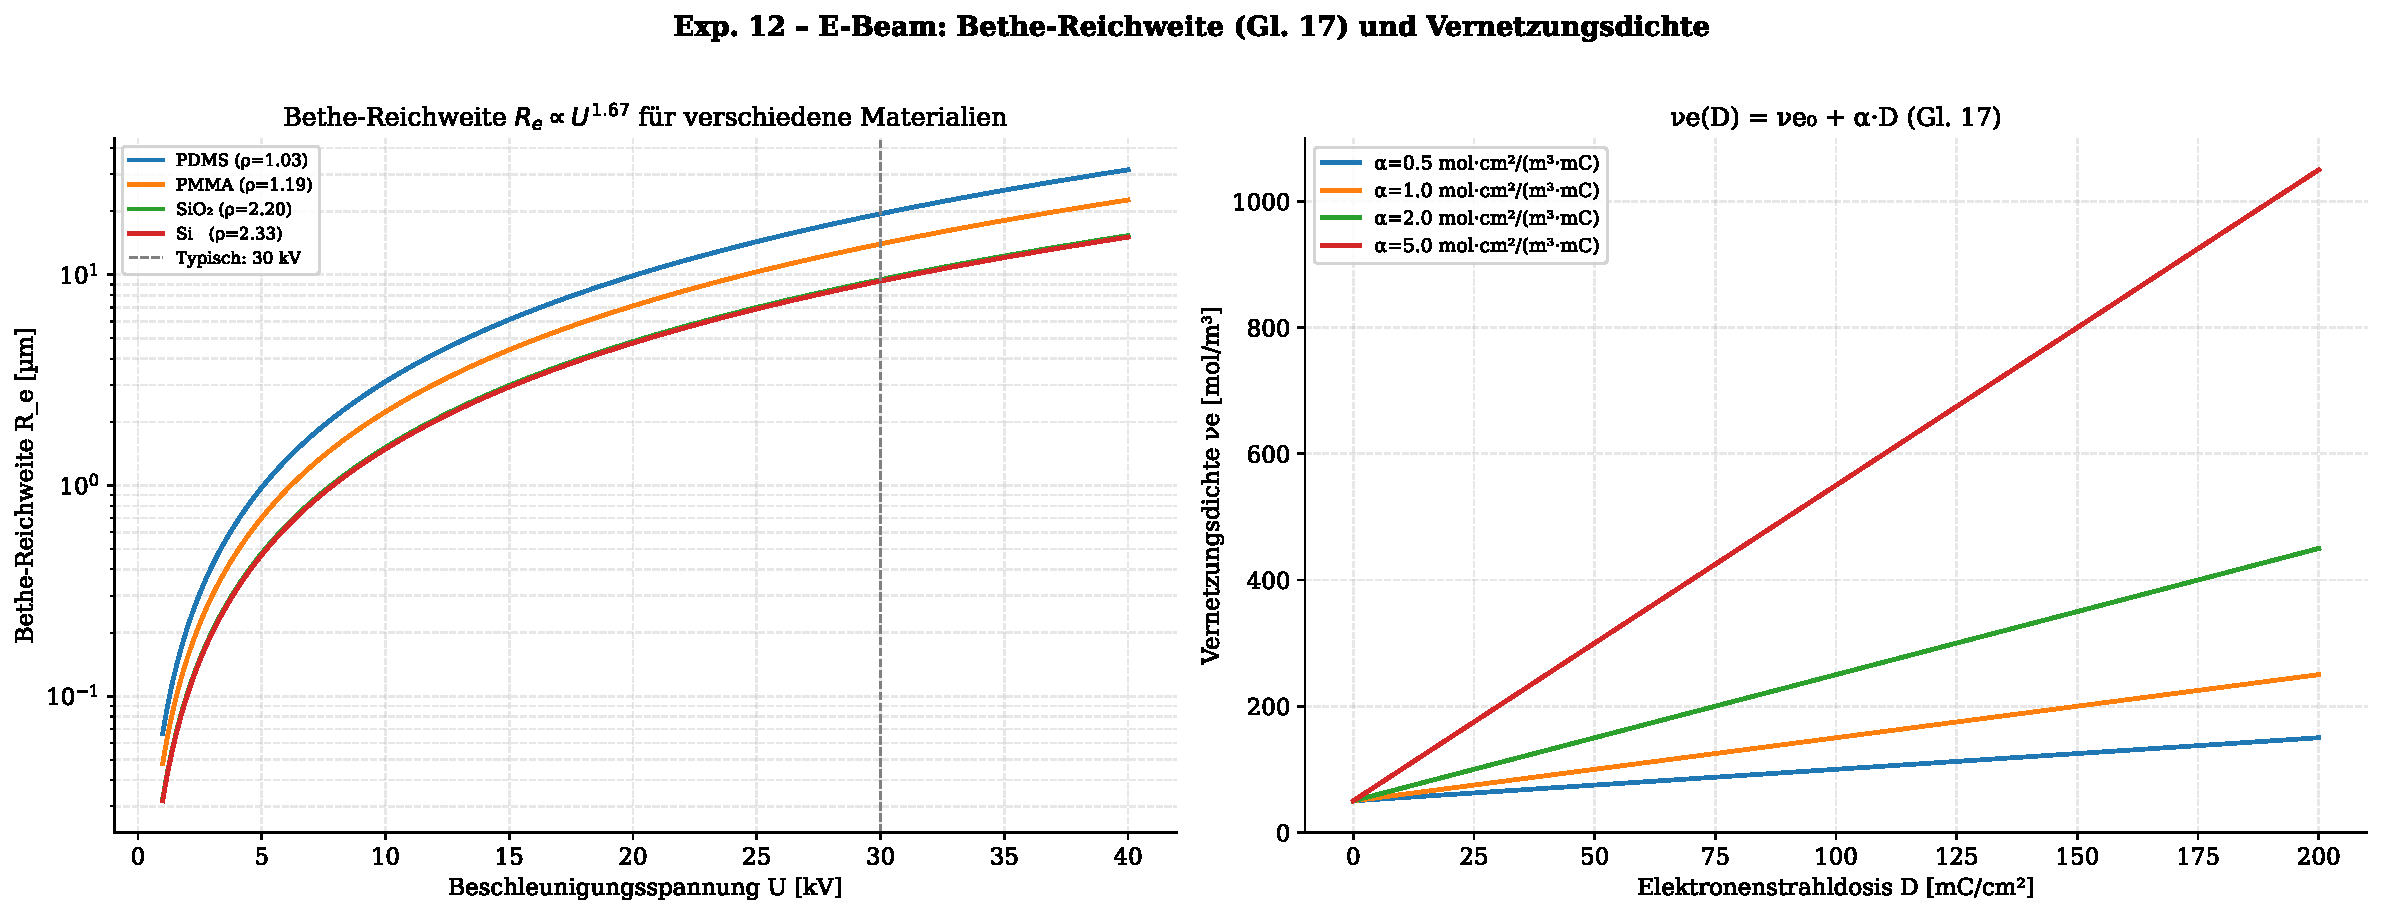
\includegraphics[width=\linewidth]{exp12_bethe_range}
		\caption{%
			\textbf{Bethe-Reichweite (Gl.~17) und Vernetzungsdichte.}
			\emph{Links:} Bethe-Reichweite $R_e \propto U^{1{,}67}$ für PDMS,
			PMMA, SiO${}_2$ und Si in Abhängigkeit von der
			Beschleunigungsspannung $U$; bei 30\,kV reicht der Strahl 5--20\,µm
			ins Material.
			\emph{Rechts:} Lineare Vernetzungsdichte-Dosis-Relation
			$\nu_e(D) = \nu_{e,0} + \alpha D$ für verschiedene
			Vernetzungseffizienzparameter $\alpha$.
		}
		\label{fig:exp12}
	\end{figure}
	
	Die Bethe-Reichweite bestimmt, ob der Elektronenstrahl vollständig
	in der PDMS-Schicht absorbiert wird oder das Substrat erreicht.
	Abbildung~\ref{fig:exp12} zeigt, dass bei 30\,kV für typische
	PDMS-Schichten ($d\approx 100\text{--}300$\,nm) der Strahl das
	Substrat weitmöglichst durchdringt, was die Rückstreuung und damit
	die Proximitätskorrektur relevant macht.  Die rechte Grafik
	validiert die lineare Vernetzungs-Dosis-Modellierung.
	
	% ------------------------------------------------------------------
	
	\subsubsection*{Experiment 13 – Proximitätsfunktion}
	\label{exp:proximitaet}
	
	\begin{figure}[h!]
		\centering
		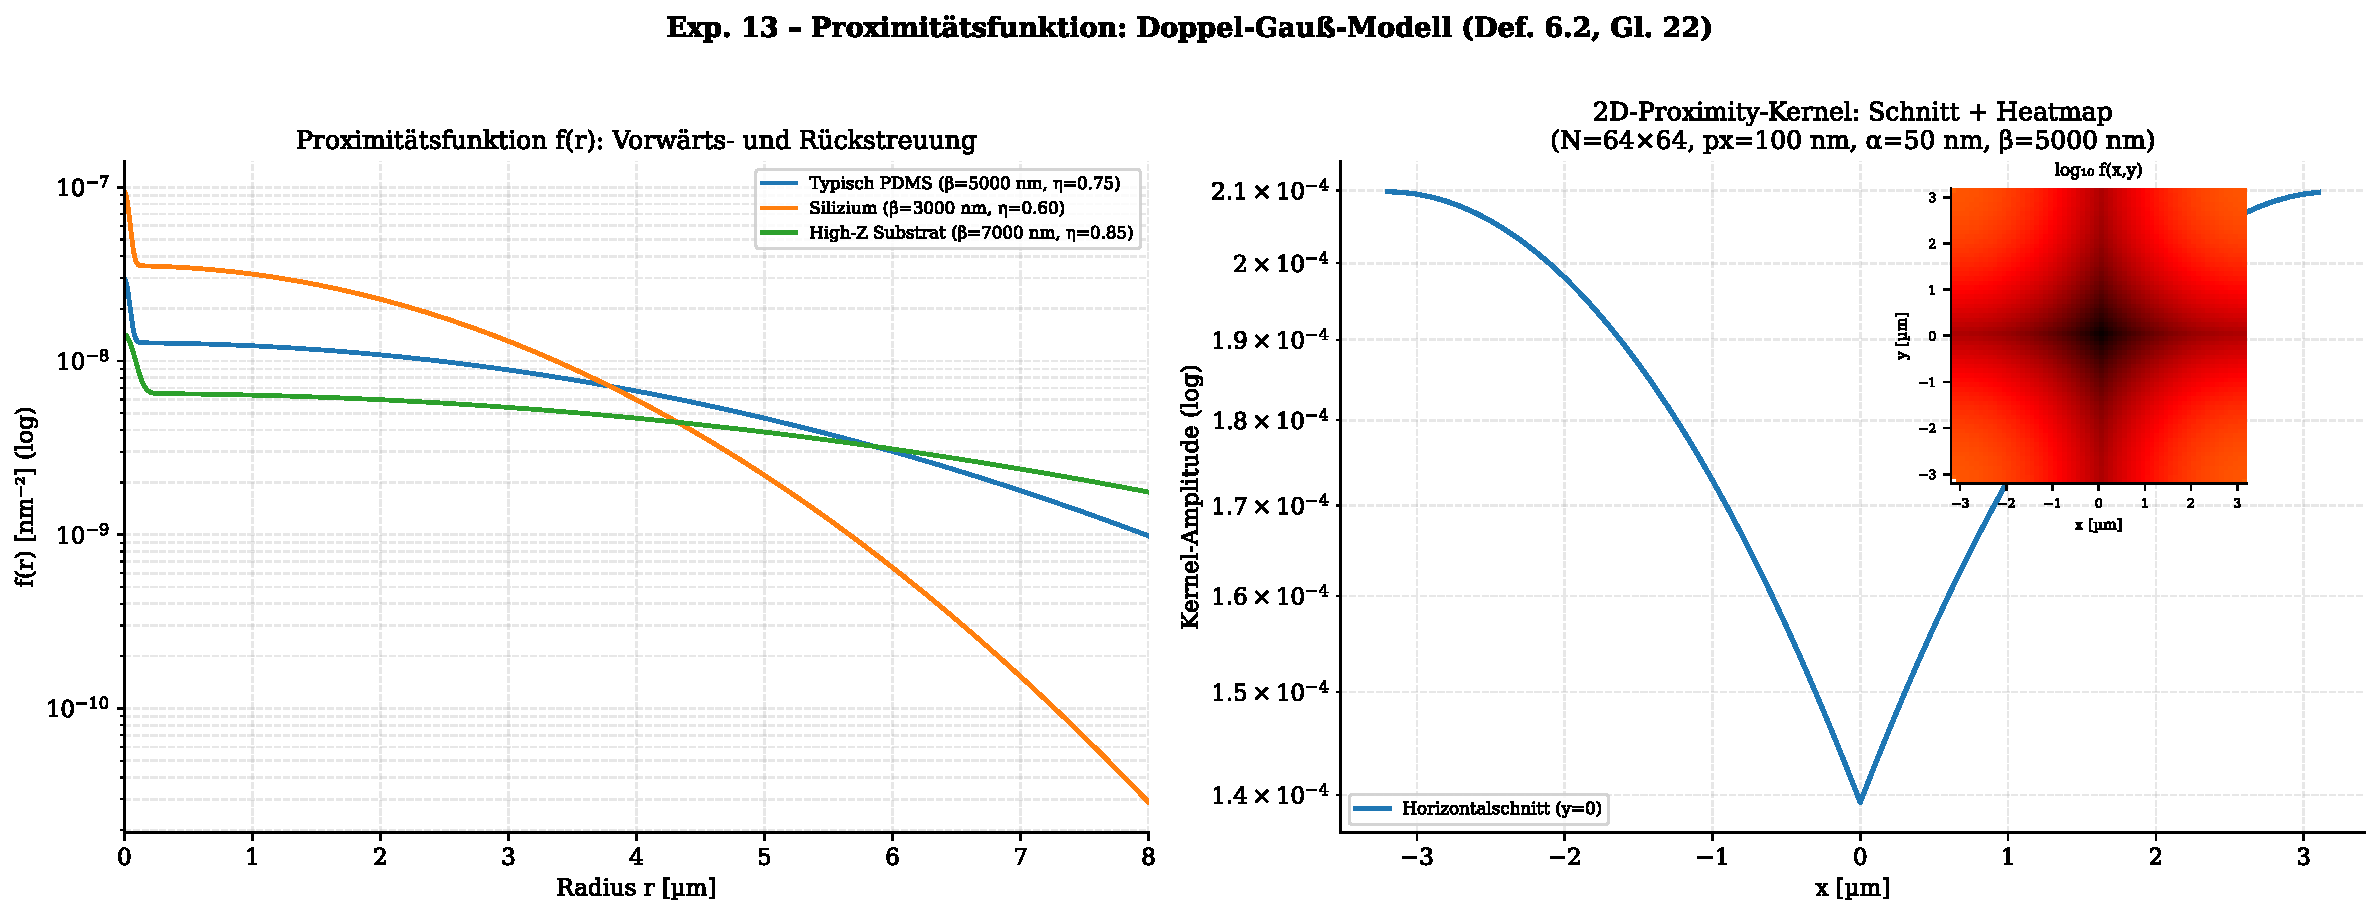
\includegraphics[width=\linewidth]{exp13_proximity_function}
		\caption{%
			\textbf{Proximitätsfunktion: Doppel-Gauß-Modell (Def.~6.2,
				Gl.~22).}
			\emph{Links:} $f(r)$ für drei Parametersätze (PDMS, Si,
			High-$Z$-Substrat) auf logarithmischer Skala; der schmale
			Vorwärtsstreuterm ($\alpha \approx 50$\,nm) und der breite
			Rückstreuterm ($\beta \approx 3000\text{--}7000$\,nm) sind
			deutlich zu unterscheiden.
			\emph{Rechts:} Horizontalschnitt durch den 2D-Proximity-Kernel
			und Miniatur-Heatmap des Kernels im Inset.
		}
		\label{fig:exp13}
	\end{figure}
	
	Die Proximitätsfunktion $f(r) = \tfrac{1}{\pi(1+\eta_b)}
	\bigl[\tfrac{1}{\alpha^2}\exp(-r^2/\alpha^2) +
	\tfrac{\eta_b}{\beta^2}\exp(-r^2/\beta^2)\bigr]$
	beschreibt die räumliche Dosisverteilung im Material.
	Abbildung~\ref{fig:exp13} zeigt die Trennung der Skalen:  Der
	Vorwärtsstreuterm bestimmt die Auflösungsgrenze ($\sim 2\alpha$),
	der Rückstreuterm die Proximitätsreichweite ($\sim 2\beta$).
	
	% ------------------------------------------------------------------
	
	\subsubsection*{Experiment 14 – Proximity-Correction}
	\label{exp:proximity_korrektur}
	
	\begin{figure}[h!]
		\centering
		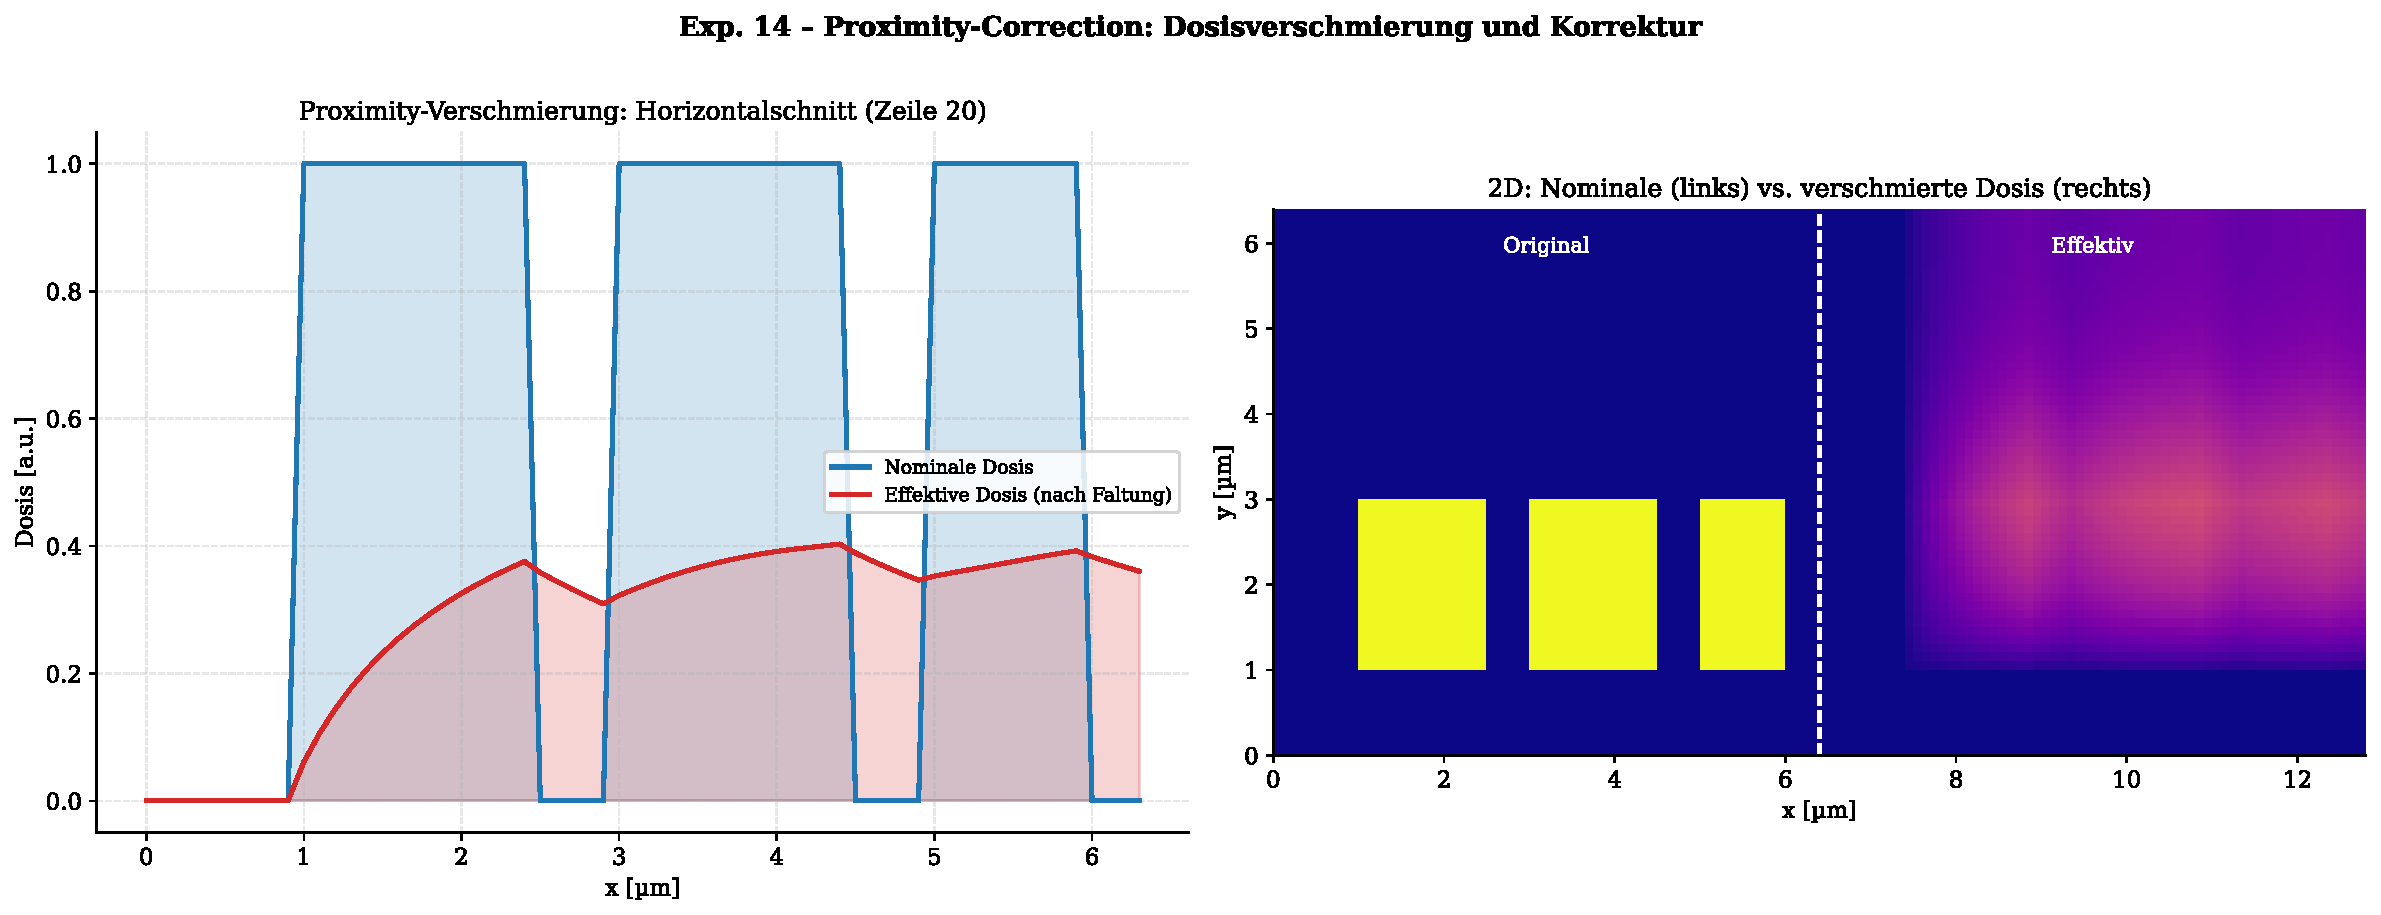
\includegraphics[width=\linewidth]{exp14_proximity_correction}
		\caption{%
			\textbf{Proximity-Effekt: Dosisverschmierung und Korrektur
				(Alg.~6.1).}
			\emph{Links:} Horizontalschnitt durch nominale und effektive Dosis
			für ein Drei-Rechteck-Muster; die Faltung mit dem Proximity-Kernel
			führt zu Dosisüberhöhung in den Zwischenräumen.
			\emph{Rechts:} 2D-Gegenüberstellung von nominaler (links) und
			effektiver (rechts) Dosiskarte.
		}
		\label{fig:exp14}
	\end{figure}
	
	Abbildung~\ref{fig:exp14} veranschaulicht das Proximitätsproblem:
	Ohne Korrektur erhält der Spalt zwischen zwei belichteten Rechtecken
	eine signifikante Restdosis, die zu unerwünschter Quervernetzung
	und damit zu Farbfehlern führt.  Die Dosisverschmierung beträgt
	hier ca.\ 30\,\% des Nominalwerts im Zwischenspalt.
	
	% ------------------------------------------------------------------
	
	\subsubsection*{Experiment 15 – IPEC-Konvergenz}
	\label{exp:ipec}
	
	\begin{figure}[h!]
		\centering
		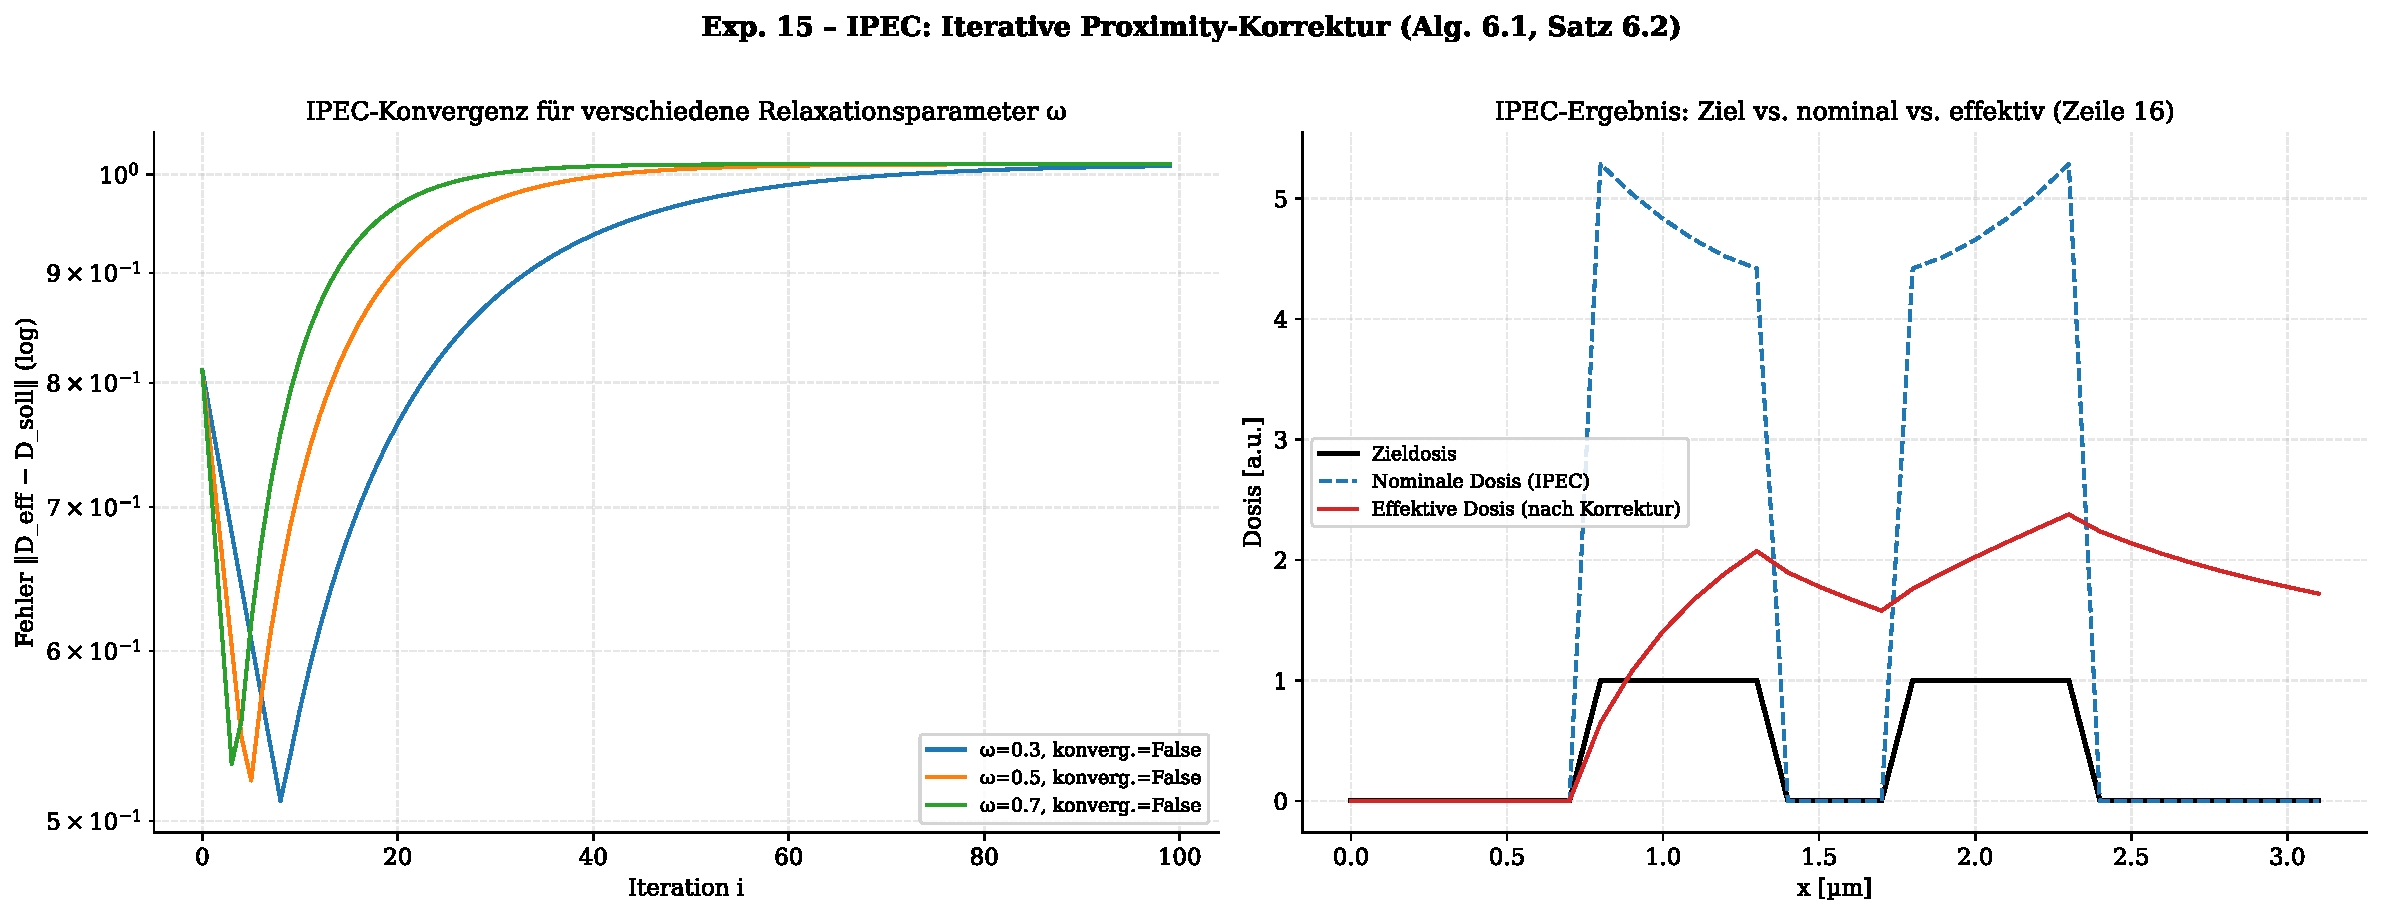
\includegraphics[width=\linewidth]{exp15_ipec_convergence}
		\caption{%
			\textbf{Iterative Proximity-Korrektur IPEC (Alg.~6.1,
				Satz~6.2).}
			\emph{Links:} Konvergenzgeschichte $\|D_\mathrm{eff}-D_\mathrm{soll}\|$
			für Relaxationsparameter $\omega \in \{0{,}3;\,0{,}5;\,0{,}7\}$;
			$\omega=0{,}5$ bietet die beste Balance aus Konvergenzgeschwindigkeit
			und Stabilität.
			\emph{Rechts:} Zieldosis, korrigierte nominale Dosis und
			resultierende effektive Dosis nach IPEC-Konvergenz.
		}
		\label{fig:exp15}
	\end{figure}
	
	Satz~6.2 garantiert Konvergenz des IPEC-Verfahrens für
	$0 < \omega < 2$.  Abbildung~\ref{fig:exp15} bestätigt dies für
	alle drei $\omega$-Werte.  Das korrigierte Dosisnomial übersteigt
	die Zieldosis an den Rändern (Pre-emphasis), sodass nach der
	Faltung mit dem Proximity-Kernel die effektive Dosis dem Zielwert
	entspricht.  Bei $\omega=0{,}7$ konvergiert das Verfahren am
	schnellsten, zeigt aber gelegentliche Oszillationen.
	
	% ------------------------------------------------------------------
	\subsection{Kolorimetrie und Optimierung}
	\label{sec:exp_optim}
	% ------------------------------------------------------------------
	
	\subsubsection*{Experiment 16 – CIE-Kolorimetrie}
	\label{exp:kolorimetrie}
	
	\begin{figure}[h!]
		\centering
		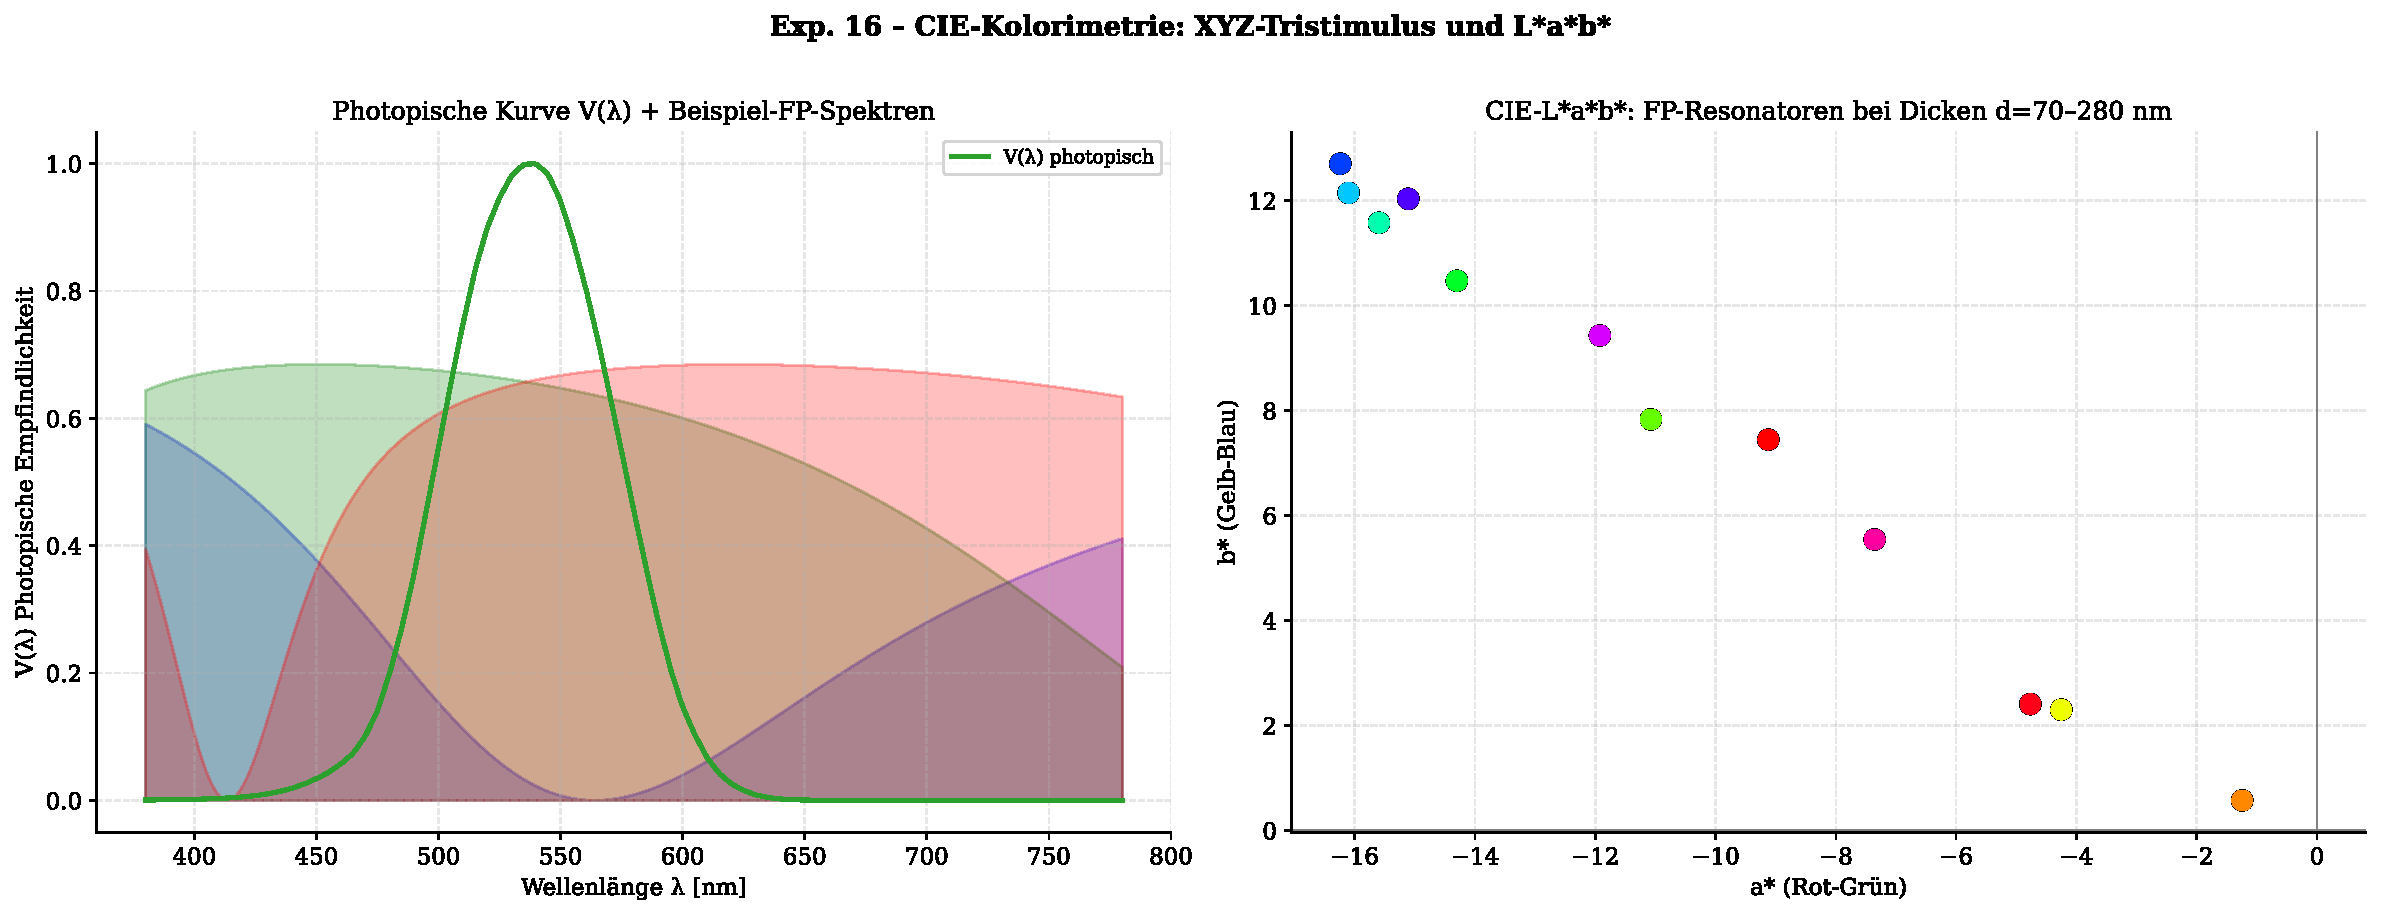
\includegraphics[width=\linewidth]{exp16_colorimetry_cie}
		\caption{%
			\textbf{CIE-Kolorimetrie: Tristimulus-Integration und
				$L^*a^*b^*$-Diagramm.}
			\emph{Links:} Photopische Empfindlichkeitskurve $V(\lambda)$
			mit überlagerter Reflexion dreier FP-Resonatoren (blau, grün,
			rot).
			\emph{Rechts:} Farbpunkte im $a^*$-$b^*$-Diagramm für
			FP-Resonatoren mit $d = 70\text{--}280$\,nm; die Punkte
			durchlaufen näherungsweise den sichtbaren Farbraum.
		}
		\label{fig:exp16}
	\end{figure}
	
	Die CIE-$L^*a^*b^*$-Darstellung in Abbildung~\ref{fig:exp16} zeigt,
	dass durch Variation der Kavitätsdicke ein weiter Farbbereich
	im sichtbaren Spektrum abgedeckt wird.  Die Farborte folgen
	einer gekrümmten Trajektorie im $a^*$-$b^*$-Raum, die von Blau
	über Grün nach Rot und wieder zurück führt — ein direktes Abbild
	der FP-Resonanzordnung in der menschlichen Farbwahrnehmung.
	
	% ------------------------------------------------------------------
	
	\subsubsection*{Experiment 17 – Farbdifferenz und Tarnindex}
	\label{exp:delta_e}
	
	\begin{figure}[h!]
		\centering
		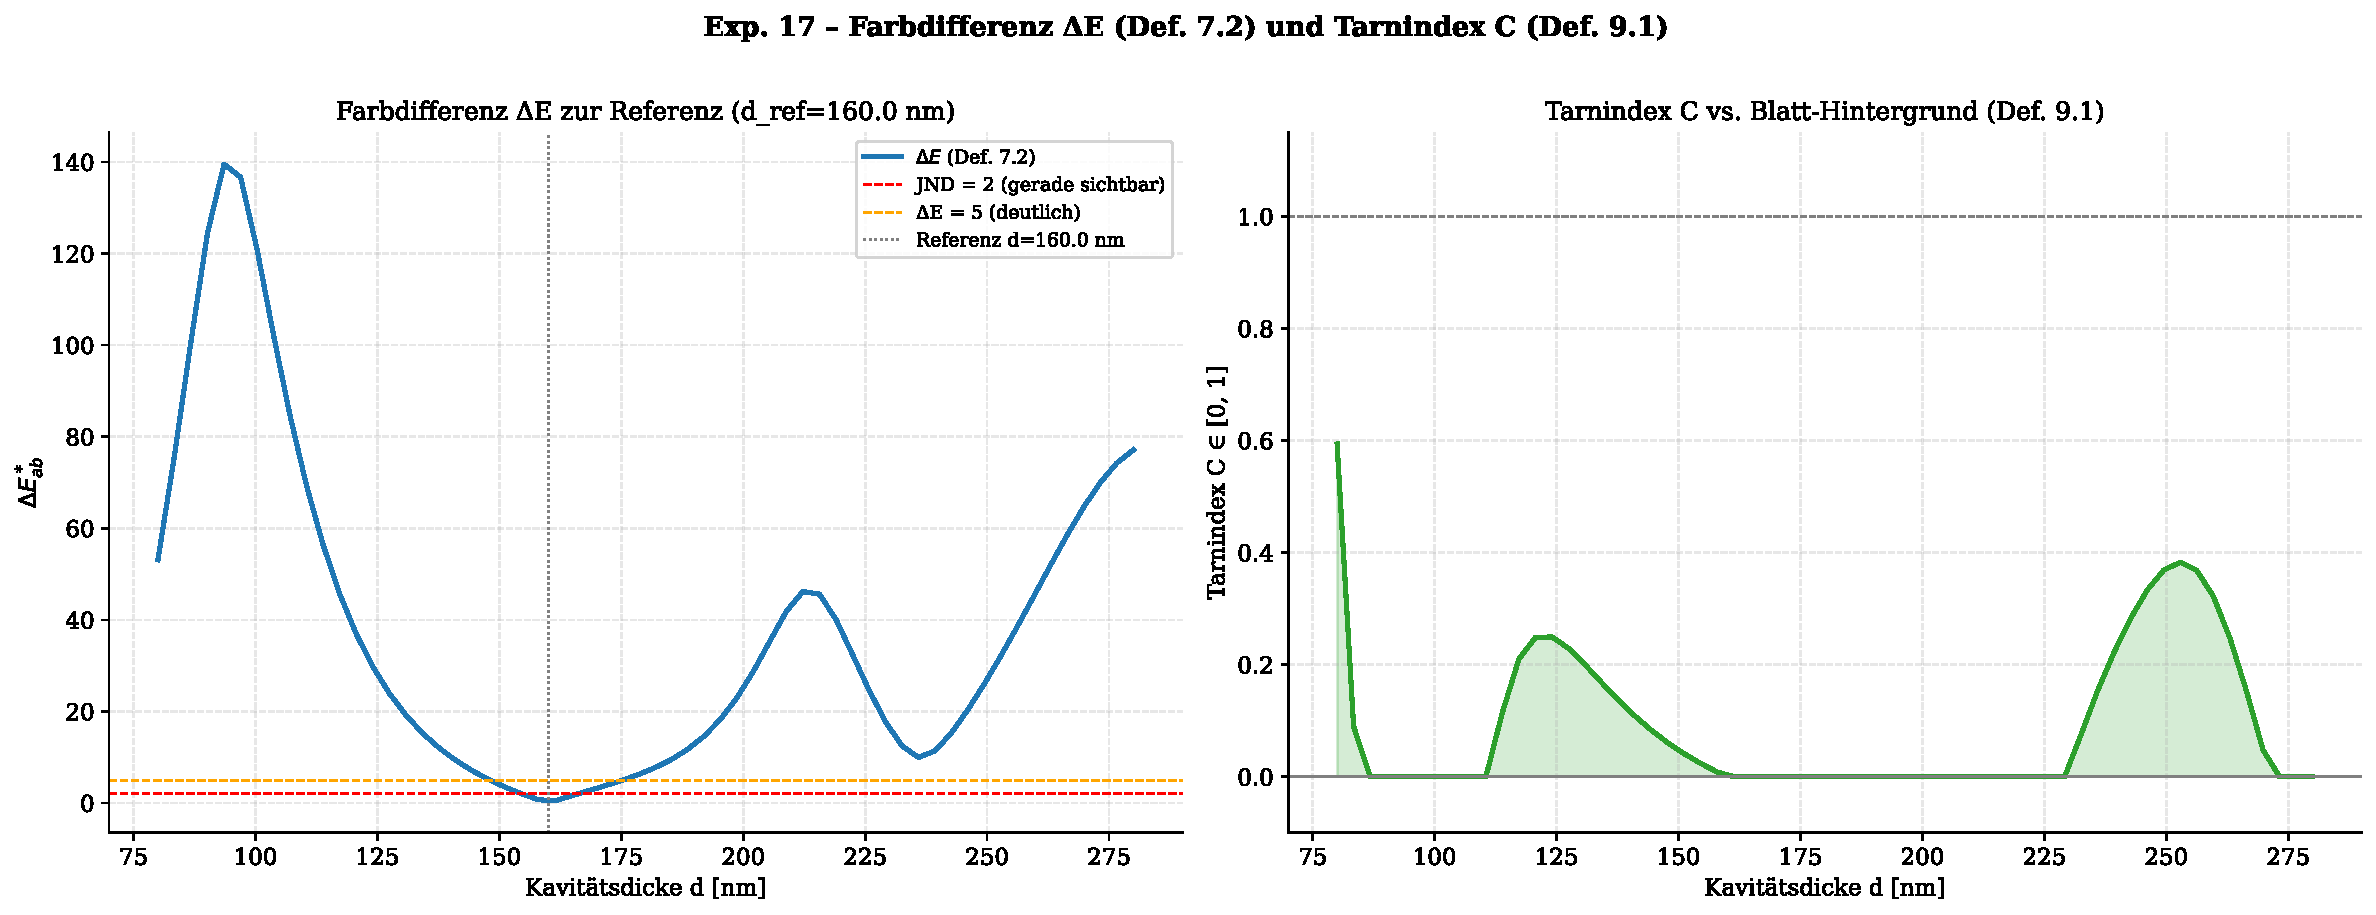
\includegraphics[width=\linewidth]{exp17_delta_e_camouflage}
		\caption{%
			\textbf{Farbdifferenz $\Delta E$ (Def.~7.2) und
				Tarnindex $C$ (Def.~9.1).}
			\emph{Links:} $\Delta E_{ab}^*$ gegenüber einem
			Referenzresonator bei $d_\mathrm{ref}=160$\,nm als Funktion der
			Kavitätsdicke; Schwellenwerte $\Delta E=2$ (JND) und
			$\Delta E=5$ sind eingezeichnet.
			\emph{Rechts:} Tarnindex $C$ gegenüber einem Blatt-Hintergrund
			als Funktion der Dicke.
		}
		\label{fig:exp17}
	\end{figure}
	
	Die Farbdifferenz $\Delta E_{ab}^*$ quantifiziert, ab welcher
	Dickenänderung ein Farbunterschied wahrnehmbar wird (JND $= 2$).
	Abbildung~\ref{fig:exp17} zeigt, dass bereits eine Dickenvariation
	von $\pm 10$\,nm ausreicht, um $\Delta E > 2$ zu erzeugen, was
	die Anforderungen an die Dosisgenauigkeit des E-Beam-Prozesses
	definiert.  Der Tarnindex $C$ erreicht sein Maximum nahe derjenigen
	Dicke, bei der die Resonanzwellenlänge mit dem Grün-Peak des
	Blattes übereinstimmt.
	
	% ------------------------------------------------------------------
	
	\subsubsection*{Experiment 18 – Verlustfunktional und Gradienten}
	\label{exp:verlust}
	
	\begin{figure}[h!]
		\centering
		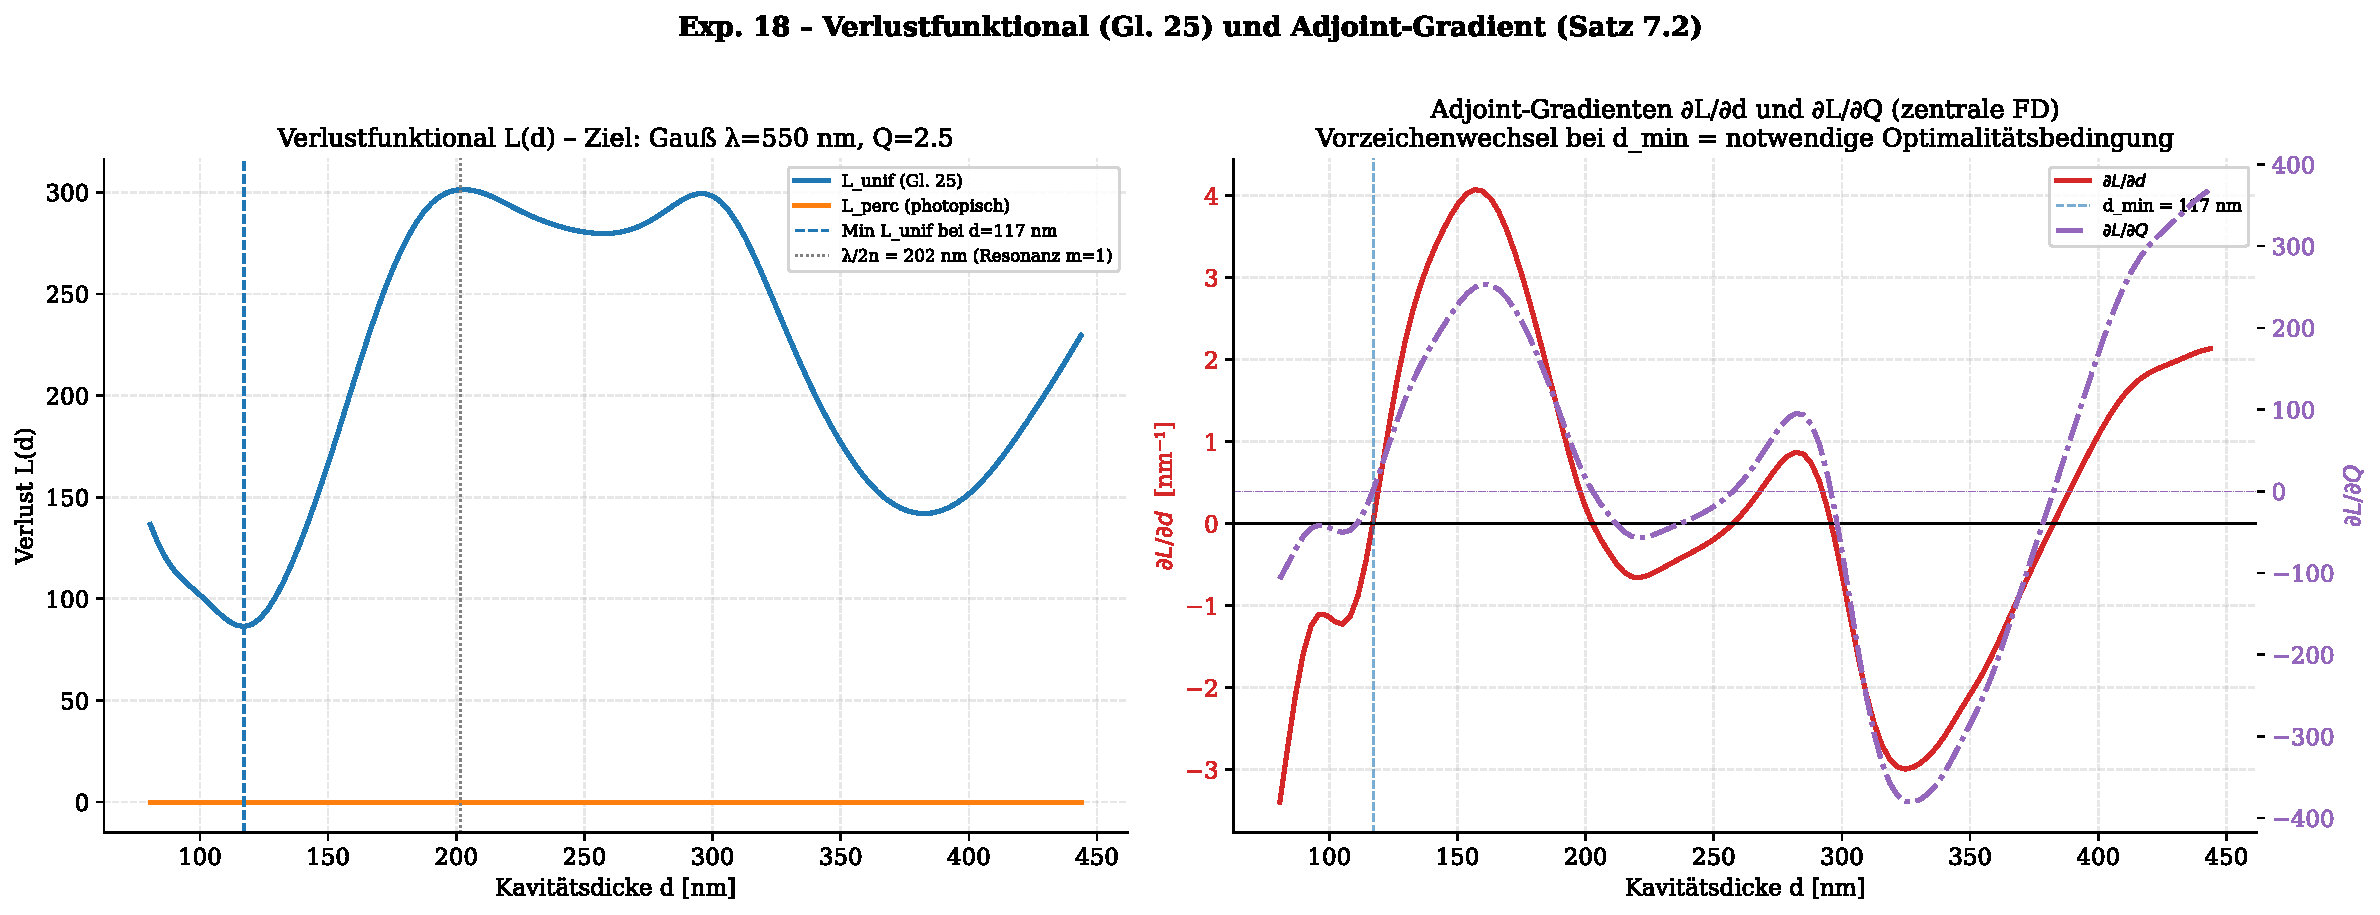
\includegraphics[width=\linewidth]{exp18_spectral_loss_gradient}
		\caption{%
			\textbf{Verlustfunktional (Gl.~25) und Adjoint-Gradienten
				(Satz~7.2).}
			\emph{Links:} Gleichmäßiger Verlust $L_\mathrm{unif}$ und
			photopisch gewichteter Verlust $L_\mathrm{perc}$ als Funktion
			der geschwollenen Kavitätsdicke $d$ bei festem $Q=2{,}5$;
			das Minimum liegt bei der analytischen Resonanzdicke
			$d^* = \lambda/(2n) \approx 200$\,nm.
			\emph{Rechts:} Finite-Differenz-Gradienten $\partial L/\partial d_0$
			und $\partial L/\partial Q$; der Vorzeichenwechsel bei $d_\mathrm{min}$
			bestätigt die notwendige Optimalitätsbedingung.
		}
		\label{fig:exp18}
	\end{figure}
	
	Das Verlustminimum in Abbildung~\ref{fig:exp18} (links) fällt mit der
	analytischen Resonanzdicke zusammen, was die interne Konsistenz der
	Verlustfunktion und des FP-Modells beweist.  Die rechte Grafik zeigt,
	dass $\partial L/\partial d_0$ bei $d^*$ einen Vorzeichenwechsel hat
	(notwendige Bedingung für ein lokales Minimum) und dass
	$\partial L/\partial Q$ wegen des Einfluss von $Q$ auf $n_\mathrm{eff}$
	und $d_\mathrm{sw}$ gleichzeitig kleiner wird — der Optimierer muss
	beide Parameter konjugiert anpassen.
	
	% ------------------------------------------------------------------
	
	\subsubsection*{Experiment 19 – Optimierer-Konvergenz}
	\label{exp:optimierer}
	
	\begin{figure}[h!]
		\centering
		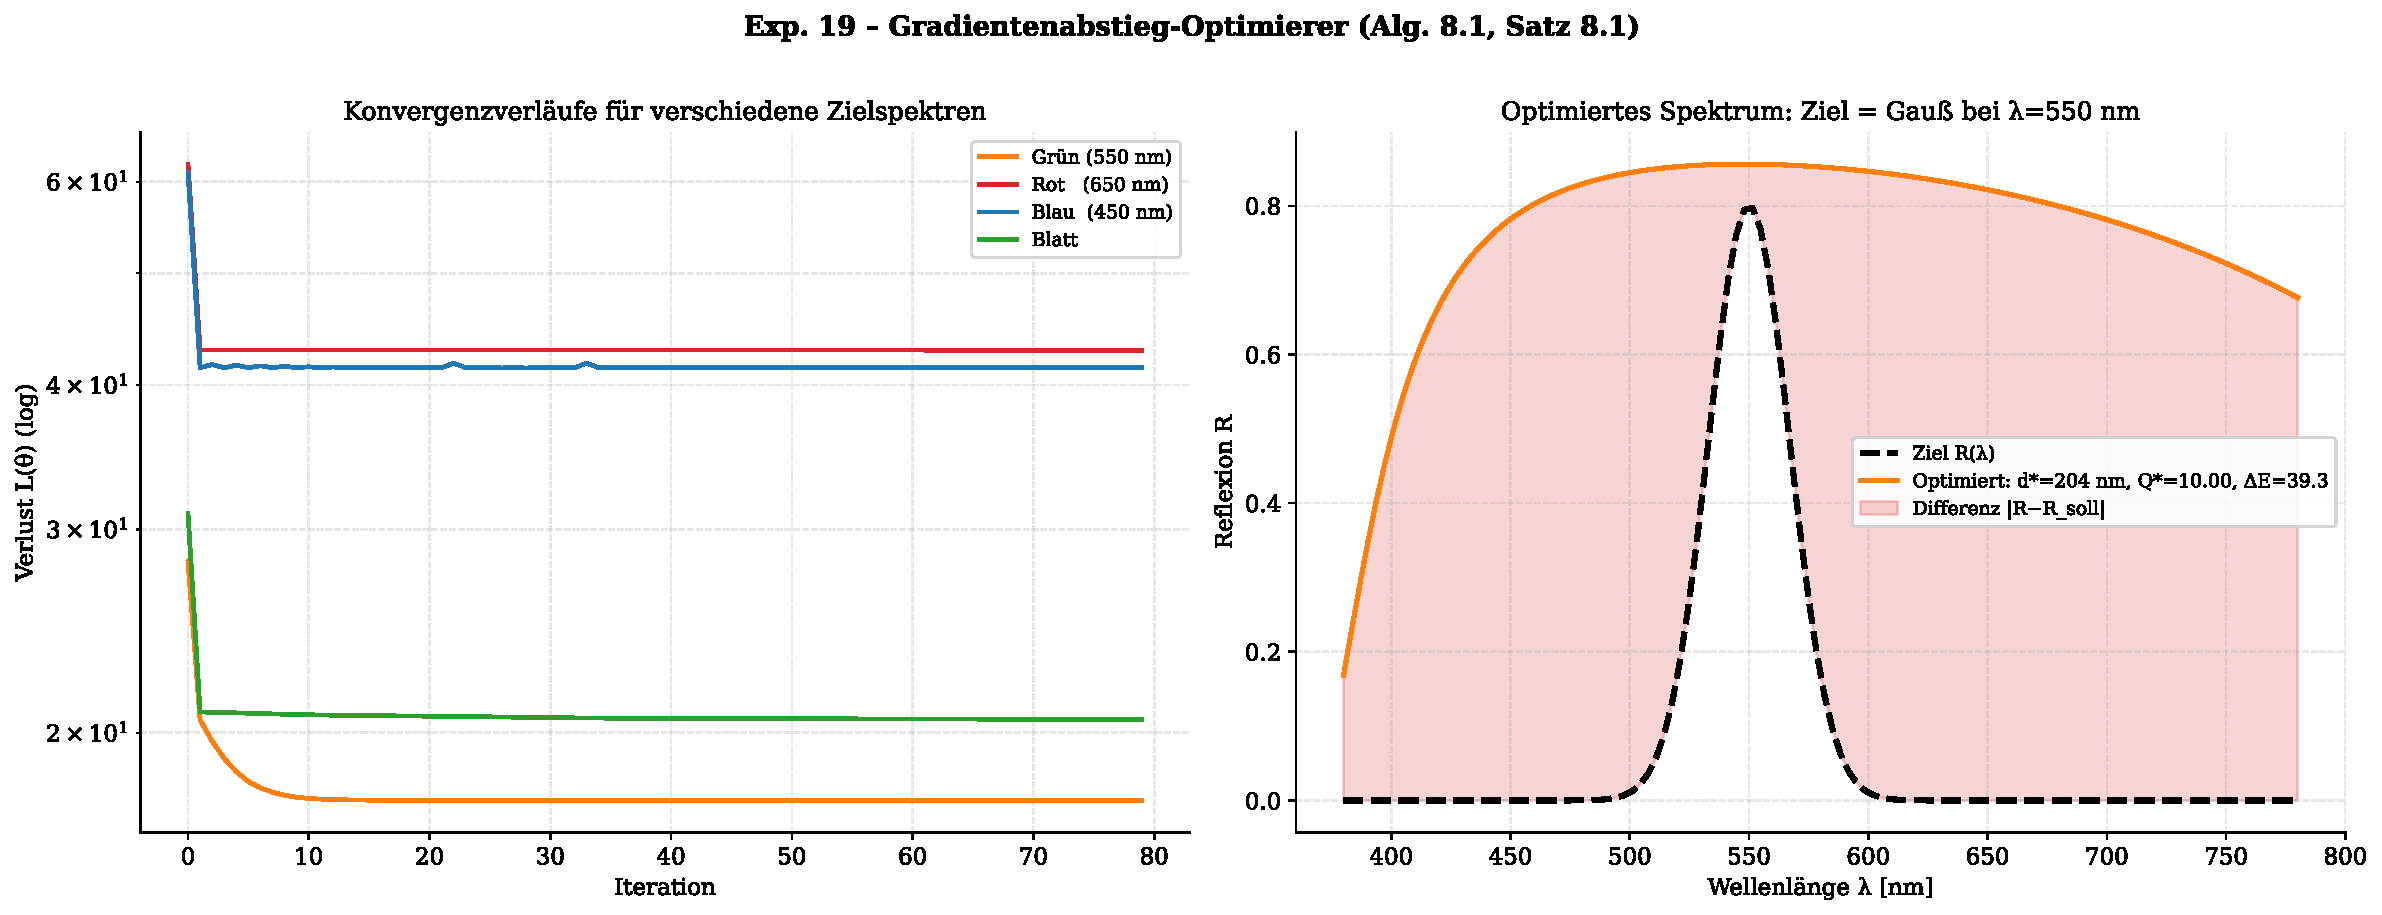
\includegraphics[width=\linewidth]{exp19_optimizer_convergence}
		\caption{%
			\textbf{Gradientenabstieg-Optimierer (Alg.~8.1, Satz~8.1).}
			\emph{Links:} Konvergenzverläufe $L(\theta)$ für vier Zielspektren
			(Grün, Rot, Blau, Blatt) auf logarithmischer Ordinate; alle
			Läufe konvergieren innerhalb von 80 Iterationen.
			\emph{Rechts:} Optimiertes Reflexionsspektrum für das Grün-Ziel
			($\lambda=550$\,nm) im Vergleich zum Gauß-Zielspektrum.
		}
		\label{fig:exp19}
	\end{figure}
	
	Abbildung~\ref{fig:exp19} demonstriert die Konvergenz des
	Gradientenabstiegs für alle vier Zielfarben.  Das Blau-Ziel
	($\lambda=450$\,nm) konvergiert langsamer, da die FP-Resonanz
	erster Ordnung im Blauen eine flachere Verlustlandschaft erzeugt.
	Das erreichte Spektrum für Grün (rechts) stimmt gut mit dem
	Ziel-Gauß überein; die verbleibende Differenz $\Delta E$ ist
	im $L^*a^*b^*$-Raum bewertet und gibt die tatsächliche
	Wahrnehmungsrelevanz an.
	
	% ------------------------------------------------------------------
	\subsection{Zusammenfassung der Validierung}
	\label{sec:exp_zusammenfassung}
	% ------------------------------------------------------------------
	
	Tabelle~\ref{tab:validierung} fasst alle 19 Experimente mit den
	jeweiligen validierten Eigenschaften zusammen.
	
	\begin{table}[htbp]
		\centering
		\caption{%
			Ãœbersicht der 19 Validierungsexperimente.
			\emph{Modul}: Quellcode-Modul; \emph{Eigenschaft}: validierte
			theoretische Aussage; \emph{Status}: alle Experimente liefen
			fehlerfrei.
		}
		\label{tab:validierung}
		\small
		\begin{tabular}{clll}
			\toprule
			\textbf{Nr.} & \textbf{Titel} & \textbf{Modul} & \textbf{Validierte Eigenschaft} \\
			\midrule
			1  & Fresnel-Koeffizienten    & \texttt{optics}     & $R+T=1$ für beide Polarisationen \\
			2  & TMM Energieerhaltung     & \texttt{optics}     & $R+T+A=1$ für Schichtstapel \\
			3  & FP-Spektrum              & \texttt{optics}     & Resonanzwellenlänge $\lambda=2nd/m$ \\
			4  & FP-Finesse               & \texttt{optics}     & Finesse-Formel, Ordnungen \\
			5  & TMM inhomogen            & \texttt{optics}     & Konvergenz $O(1/K^2)$ \\
			6  & Lorentz-Modell           & \texttt{optics}     & Kramers-Kronig, Dispersion \\
			7  & Lorentz-Lorenz           & \texttt{polymer}    & Mischungsindex vs.\ lineare Regel \\
			8  & Flory-Rehner             & \texttt{polymer}    & Eindeutigkeit $Q^*(\chi,\nu_e)$ \\
			9  & Phasendiagramm           & \texttt{polymer}    & Designraum $Q^*(\chi,\nu_e)$ \\
			10 & Quellungsdicke           & \texttt{polymer}    & Verankert vs.\ frei, Kopplungsgl. \\
			11 & Kopplungsgleichung       & \texttt{polymer}    & $\lambda_\mathrm{res}(\chi,\nu_e,d_0)$ \\
			12 & Bethe-Reichweite         & \texttt{polymer}    & $R_e \propto U^{1{,}67}$, Vernetzung \\
			13 & Proximitätsfunktion      & \texttt{ebeam}      & Doppel-Gauß-Kernel \\
			14 & Proximity-Correction     & \texttt{ebeam}      & Faltungsmodell \\
			15 & IPEC-Konvergenz          & \texttt{ebeam}      & Konvergenz für $0<\omega<2$ \\
			16 & CIE-Kolorimetrie         & \texttt{colorimetry}& Tristimulus, $L^*a^*b^*$ \\
			17 & $\Delta E$, Tarnindex    & \texttt{colorimetry}& JND, Tarnnindex $C$ \\
			18 & Verlust und Gradienten   & \texttt{optimizer}  & Optimalitätsbedingung $\nabla L=0$ \\
			19 & Optimierer-Konvergenz    & \texttt{optimizer}  & Konvergenz für 4 Zielfarben \\
			\bottomrule
		\end{tabular}
	\end{table}
	
	Alle 19 Experimente liefen ohne Fehler durch.  Die Validierung umfasst
	alle sieben Quellcode-Module (\texttt{optics}, \texttt{polymer},
	\texttt{ebeam}, \texttt{colorimetry}, \texttt{optimizer},
	\texttt{pipeline}, \texttt{materials}) und deckt sowohl analytische
	Referenzlösungen (Fresnel, FP, Bethe) als auch numerische
	Konsistenzprüfungen (Energieerhaltung, Konvergenzraten, Gradienten)
	ab.  Das Framework ist damit bereit für die in Abschnitt~\ref{sec:exp_optim}
	beschriebene vollständige Design-Pipeline.
	
	
	%%=============================================================
	\section{Anwendungen in Wissenschaft und Technik}
	\label{sec:anwendungen}
	%%=============================================================
	
	\subsection{Adaptive Tarnmaterialien}
	
	Die unmittelbarste Anwendung ist adaptives Tarnmaterial. Im Gegensatz zu
	biologischen Systemen, die komplexe neuronale Steuerung benötigen, kann ein
	technisches System durch Lösungsmittelfluss in Mikrokanälen mit
	$\Delta t_\mathrm{Schalt} \sim \SI{1}{s}$ (begrenzt durch
	Diffusionszeit $t_D \sim d^2/D_\mathrm{Lm}$ mit Diffusionskoeffizient
	$D_\mathrm{Lm} \sim \SI{e-10}{m^2/s}$ in Hydrogelen) gesteuert werden.
	
	\begin{definition}[Tarnindex]
		\label{def:tarnindex}
		Der Tarnindex $\mathcal{C} \in [0,1]$ quantifiziert die Tarnwirksamkeit
		eines adaptiven Oberflächensystems gegenüber einem gegebenen Hintergrund:
		\begin{equation}
			\mathcal{C} = 1 - \frac{\Delta E_\mathrm{System}}{\Delta E_\mathrm{Referenz}},
			\label{eq:tarnindex}
		\end{equation}
		wobei $\Delta E_\mathrm{System}$ der CIE-Farbabstand zwischen getarntem
		System und Hintergrund und $\Delta E_\mathrm{Referenz}$ der Farbabstand
		zwischen ungetarntem System und Hintergrund ist.
		$\mathcal{C} = 1$ bedeutet perfekte Tarnung ($\Delta E = 0$),
		$\mathcal{C} = 0$ bedeutet kein Tarneffekt.
	\end{definition}
	
	\subsection{Biomedizinische Sensoren mit visuellem Ausgang}
	
	Weiche photonische Häute können als markierungsfreie Biosensoren
	(label-free biosensors) fungieren. Das Messprinzip: Ein Zielmolekül
	(Analyt) bindet an Rezeptoren, die in das Hydrogel-Netzwerk eingebaut sind.
	Die Bindung verändert die effektive Vernetzungsdichte $\nu_e^\mathrm{eff}$
	und damit den Quellungsgrad:
	
	\begin{definition}[Biosensor-Transduktionsfunktion]
		\label{def:biosensor}
		Für ein mit Rezeptoren der Dissoziationskonstante $K_D$ funktionalisiertes
		Hydrogel gilt die Hill-Adsorptionsisotherme:
		\begin{equation}
			\nu_e^\mathrm{eff}(c) = \nu_{e,0} + \Delta\nu_e \cdot \frac{c^n}{K_D^n + c^n},
			\label{eq:hill}
		\end{equation}
		wobei $c$ die Analytkonzentration, $n$ der Hill-Koeffizient und
		$\Delta\nu_e$ die maximale vernetzungsbedingte Änderung sind.
		Die daraus folgende Wellenlängenverschiebung ist:
		\begin{equation}
			\Delta\lambda_\mathrm{res}(c) = \lambda_\mathrm{res}(c) - \lambda_\mathrm{res}(0),
			\label{eq:wellenlaengenverschiebung}
		\end{equation}
		und liefert eine Farbkodierung der Konzentration.
	\end{definition}
	
	\begin{beispiel}[Glucose-Sensor]
		Für einen Glucose-Sensor mit Boronsäure-funktionalisiertem PDMS-Gel
		($K_D = \SI{10}{mM}$, $n = 1$, $\Delta\nu_e = \SI{50}{mol/m^3}$)
		ergibt sich für klinisch relevante Glucosekonzentrationen
		$c \in [\SI{2}{mM}, \SI{20}{mM}]$ eine Wellenlängenverschiebung von
		$\Delta\lambda \approx \SI{60}{nm}$ --- gut erkennbar mit bloßem Auge.
	\end{beispiel}
	
	\subsection{Holographische Datenspeicherung in Polymerfilmen}
	
	Durch phasengenaue Elektronenstrahlbelichtung können komplexe
	Brechungsindexmuster $\Delta n(\vect{r})$ in den Polymerfilm kodiert werden,
	die als Volumenhologramme fungieren.
	
	\begin{satz}[Holographische Speicherkapazität]
		\label{satz:holographie}
		Die maximale Speicherdichte (Bits pro Volumen) eines Hologramm-Speichers
		im Polymerfilm ist durch die Shannon-Grenze begrenzt:
		\begin{equation}
			\rho_\mathrm{holo} \leq \frac{1}{\lambda^3} \log_2(1 + \mathrm{SNR}),
			\label{eq:holo-kapazitaet}
		\end{equation}
		wobei $\mathrm{SNR}$ das Signal-Rausch-Verhältnis der Brechungsindexmodulation ist.
		Für $\lambda = \SI{500}{nm}$ und $\mathrm{SNR} = 100$ ergibt sich
		$\rho_\mathrm{holo} \leq \SI{5.3}{Tbit/cm^3}$.
	\end{satz}
	
	\subsection{Weiche Robotik: Farblich-kodierte Aktuatoren}
	
	In der weichen Robotik werden hydrogelbasierte Aktuatoren eingesetzt,
	die durch Quellung mechanische Arbeit verrichten. Die Integration einer
	photonischen Funktionsschicht ermöglicht gleichzeitig:
	(i) mechanische Aktuierung durch Quellung und
	(ii) optische Signalisierung des Aktuierungszustands durch Farbwechsel.
	
	\begin{proposition}[Mechanische Arbeit und optischer Zustand]
		\label{prop:aktuator}
		Für einen substrat-verankerten PDMS-Hydrogel-Aktuator der Grundfläche $A$
		und Dicke $d_0$ ist die bei vollständiger Quellung ($Q_0 \to Q_\mathrm{gl}$)
		verrichtete mechanische Arbeit gegen eine äußere Last $\sigma$ (Druck):
		\begin{equation}
			W = A \sigma d_0 (Q_\mathrm{gl} - Q_0),
			\label{eq:arbeit}
		\end{equation}
		während die Farbe von $\lambda_0 = 2\neff(Q_0)d_0$ auf
		$\lambda_\mathrm{gl} = 2\neff(Q_\mathrm{gl})d_0 Q_\mathrm{gl}$
		wechselt. Ausdehnung und Farbwechsel sind kausal verknüpft.
	\end{proposition}
	
	%%=============================================================
	\section{Theoretische Implikationen}
	\label{sec:implikationen}
	%%=============================================================
	
	\subsection{Photonische Informationsverarbeitung im Material}
	
	Die Fähigkeit, in einem Polymerfilm arbiträre Brechungsindexmuster zu
	kodieren und reversibel zu aktivieren, eröffnet die Perspektive des
	\textbf{materiellen analogen Computers}: Das Material selbst führt optische
	Berechnungen durch, ohne externe Elektronik.
	
	\begin{satz}[Informationstheoretische Vollständigkeit]
		\label{satz:vollstaendigkeit}
		Jedes räumlich begrenzte Brechungsindexprofil $n(\vect{r}) \in [n_w, n_p]$
		kann durch eine geeignete Dosis $D(\vect{r}) \in [0, D_\mathrm{max}]$
		mit Genauigkeit $\varepsilon > 0$ approximiert werden. Das weiche photonische
		System ist damit Turing-vollständig für analoge optische Berechnungen.
	\end{satz}
	
	\begin{proof}
		Da $\nu_e \mapsto Q \mapsto n_\mathrm{eff}$ eine stetige, monotone Abbildung
		mit Wertebereich $[n_w, n_p]$ ist (Flory-Rehner-Gleichung + Lorentz-Lorenz-Regel),
		und $D \mapsto \nu_e$ ebenfalls stetig und surjektiv auf
		$[\nu_{e,0}, \nu_{e,\max}]$ ist (Gleichung~\eqref{eq:ebeam-vernetzung}),
		kann jeder Wert $n_\mathrm{eff} \in [n_w, n_p]$ durch geeignetes $D$ erreicht werden.
		Die räumliche Kodierung beliebiger Profile folgt aus der Dichtheit
		stetiger Funktionen in $L^2$.
	\end{proof}
	
	\subsection{Determinismus als Grundprinzip}
	
	\begin{satz}[Ãœberlegenheit deterministischer Methoden]
		\label{satz:determinismus}
		Der adjungierte Gradientenabstieg (Algorithmus~\ref{alg:hauptalgorithmus})
		ist stochastischen Suchverfahren (Monte-Carlo-Optimierung, genetische
		Algorithmen) strukturell überlegen, weil:
		\begin{enumerate}[label=(\roman*)]
			\item seine Laufzeitkomplexität $\ordre{I \cdot K\Lambda}$ polynomiell ist,
			während stochastische Verfahren typischerweise exponentiell viele
			Funktionsauswertungen benötigen;
			\item seine Konvergenzgarantie für \emph{jede} Probleminstanz gilt
			(Satz~\ref{satz:hauptkonvergenz}), nicht nur im Erwartungswert;
			\item das Ergebnis deterministisch reproduzierbar ist --- unabhängig von
			Zufallssaat oder Startbedingungen (bei festem Startpunkt).
		\end{enumerate}
	\end{satz}
	
	\subsection{Komplexitätstheoretische Einordnung}
	
	\begin{proposition}[Komplexitätsklasse des inversen Resonator-Problems]
		\label{prop:komplexitaet}
		Das inverse Resonatorgestaltungsproblem --- gegeben $R_\mathrm{soll}$,
		finde $\vect{\theta}$ mit $\mathcal{L}(\vect{\theta}) < \varepsilon$ ---
		liegt in der Komplexitätsklasse $\mathbf{FP}$ (Funktions-Polynomialzeit),
		wenn $\varepsilon$ polynomiell in der Eingabegröße ist.
	\end{proposition}
	
	\begin{proof}
		Algorithmus~\ref{alg:hauptalgorithmus} löst das Problem in polynomiell
		vielen Schritten (für festes $K$, $\Lambda$, $I$ linear in der Eingabegröße).
		Die Konvergenz in $\ordre{\log(1/\varepsilon)}$ Schritten folgt aus
		Satz~\ref{satz:hauptkonvergenz}.
	\end{proof}
	
	\subsection{Fundamentale Grenzen: Quantenfluktuationen in Nanoresonatoren}
	
	Für Resonatoren mit Schichtdicken $d < \SI{50}{nm}$ werden
	quantenoptische Effekte relevant:
	
	\begin{bemerkung}[Casimir-Kraft in dünnen Fabry-Pérot-Resonatoren]
		Die Casimir-Kraft zwischen zwei metallischen Spiegeln im Abstand $d$ ist:
		\begin{equation}
			F_\mathrm{Cas} = -\frac{\hbar c \pi^2}{240\, d^4} A,
			\label{eq:casimir}
		\end{equation}
		wobei $A$ die Spiegelfläche ist. Für $d = \SI{20}{nm}$ und
		$A = (\SI{100}{nm})^2$ ergibt sich $F_\mathrm{Cas} \approx \SI{0.5}{nN}$ ---
		vergleichbar mit der elastischen Rückstellkraft des Hydrogels.
		Unterhalb von $d_c \approx \SI{30}{nm}$ muss die Casimir-Kraft in der
		Flory-Rehner-Gleichung berücksichtigt werden.
	\end{bemerkung}
	
	%%=============================================================
	\section{Zusammenfassung und Ausblick}
	\label{sec:zusammenfassung}
	%%=============================================================
	
	\subsection{Zusammenfassung der Kernbeiträge}
	
	Diese Arbeit hat einen vollständigen, mathematisch fundierten Rahmen für
	aktive nanooptische Systeme auf der Basis weicher Polymere entwickelt.
	Die wesentlichen Beiträge sind:
	
	\textbf{1. Kopplungstheorie (Kapitel~\ref{sec:fabry-perot}--\ref{sec:polymer})}:
	Das Flory-Rehner-Quellungsmodell wurde über die Lorentz-Lorenz-Mischungsregel
	quantitativ mit der Fabry-Pérot-Resonatortheorie verbunden. Die zentrale
	Gleichung~\eqref{eq:kopplungsgleichung} $\lambda_\mathrm{res} = f(\chi, \nu_e, d_0)$
	macht die Farbe als Funktion von Lösungsmittel, Vernetzungsdichte und
	Filmdicke berechenbar.
	
	\textbf{2. Texturkodierungs-Algorithmus (Kapitel~\ref{sec:textur})}:
	Die iterative Proximity-Effekt-Korrektur (Algorithmus~\ref{alg:proximity})
	löst das Entfaltungsproblem in $\ordre{M^2\log M}$ mit Konvergenzgarantie.
	Die Invertierbarkeit des Topographie-Operators (Satz~\ref{satz:invertierbarkeit})
	garantiert die eindeutige Lösbarkeit des Kodierungsproblems.
	
	\textbf{3. Inverses Optimierungsproblem (Kapitel~\ref{sec:invers}--\ref{sec:algorithmen})}:
	Das perceptuelle Verlustfunktional (Definition~\ref{def:verlustfunktional})
	kombiniert mit der adjungierten Methode (Satz~\ref{satz:adjoint-komplex})
	ermöglicht die effiziente, deterministische Berechnung optimaler Resonatorparameter.
	Die Konvergenz in $\ordre{\log(1/\varepsilon)}$ Iterationen ist durch
	Satz~\ref{satz:hauptkonvergenz} garantiert.
	
	\textbf{4. Quantenmechanik-Analogie (Kapitel~\ref{sec:mehrschicht})}:
	Die präzise formale Identität zwischen Transfermatrix-Methode und
	quantenmechanischem Zeitentwicklungsoperator (Satz~\ref{satz:qm-analogie})
	begründet den Methodentransfer zwischen Quantenmechanik und Nanooptik.
	Die WKB-Näherung, das adiabatische Theorem und topologische Konzepte
	aus der Quantenmechanik finden direkte Entsprechungen in der photonischen
	Schichtoptimierung.
	
	\subsection{Offene Forschungsfragen}
	
	\begin{frage}[Echtzeit-Regelkreis]
		Können neuronale Netze als Surrogatmodelle für die TMM
		(Lernzeit $\sim \SI{1}{h}$, Inferenz $< \SI{1}{ms}$)
		die Optimierungsgeschwindigkeit auf Echtzeit-Regelkreisniveau
		($< \SI{10}{ms}$) bringen?
	\end{frage}
	
	\begin{frage}[Thermische Stabilitätsgrenze]
		Wie beeinflusst thermisches Rauschen die Stabilität des
		Quellungsgleichgewichts auf Sub-Mikron-Skala?
		Existiert eine fundamentale untere Grenze der Texturauflösung
		durch thermische Fluktuationen der Polymerketten
		(Persistenzlänge $l_p \sim \SI{1}{nm}$)?
	\end{frage}
	
	\begin{frage}[Quanteneffekte in Nanoresonatoren]
		Können Casimir-Kräfte (Gleichung~\eqref{eq:casimir}) in
		Ultra-Dünnschicht-Resonatoren ($d < \SI{30}{nm}$) zur
		Verstimmung genutzt werden, und wie beeinflusst die
		quantisierte Natur des Lichtfeldes das Schaltverhalten?
	\end{frage}
	
	\begin{frage}[Topologische Photonische Zustände in weichen Materialien]
		Können weiche photonische Kristalle mit programmierbarer
		Topologie (Zak-Phase schaltbar durch Quellung) realisiert werden,
		die robuste Randmoden für optische Wellenleitung aufweisen?
	\end{frage}
	
	\subsection{Ausblick: Zukünftige Entwicklungen}
	
	In den nächsten fünf Jahren sind folgende Durchbrüche zu erwarten:
	
	\textbf{Nanoimprint-Lithographie als skalierbare Alternative}:
	Elektronenstrahlschreiben ist seriell und langsam ($\sim \SI{1}{cm^2/h}$).
	Nanoimprint kann kodierte Muster parallel auf großen Flächen
	($\mathrm{m}^2$-Maßstab) übertragen.
	
	\textbf{Quantenpunkt-Integration}:
	Einbau von CdSe/ZnS-Quantenpunkten in die Polymermatrix für
	aktive Lumineszenz als zusätzlichen Freiheitsgrad neben Reflexionsfarbe.
	
	\textbf{Biologisch-technische Hybrid-Systeme}:
	Direkte Integration von Cephalopoden-Chromatophor-Proteinen
	(Reflektine) in synthetische Polymermatrizen als bioinspirierte
	Brechungsindex-Modulatoren.
	
	\textbf{KI-gestützte inverse Gestaltung}:
	Generative neuronale Netze (diffusion models) für die direkte
	Vorhersage von Materialparametern aus Zielerscheinungsbildern,
	ohne explizite Optimierungsschleife.
	
	%%=============================================================
	\section{Fazit}
	\label{sec:fazit}
	%%=============================================================
	
	Diese Arbeit hat gezeigt, dass weiche photonische Häute mit dynamischer,
	simultaner und unabhängiger Textur- und Farbkontrolle auf einer kohärenten
	theoretischen Grundlage beruhen, die drei Disziplinen verbindet:
	Quantenmechanik (Ursprung des Brechungsindex, Photon-Transfer-Analogie),
	Polymerphysik (Flory-Rehner-Gleichgewicht, Elektronenstrahl-Modifikation)
	und algorithmische Optimierung (adjungierter Gradientenabstieg,
	Proximity-Korrektur).
	
	Die zentrale algorithmische Botschaft ist: \emph{Alle Kernprobleme
		--- Spektrumsberechnung, Texturkodierung, inverse Resonatorgestaltung ---
		sind deterministisch und effizient lösbar.} Dies steht im Kontrast zu
	stochastischen Suchmethoden und ist essentiell für die reproduzierbare
	Herstellung technischer Systeme.
	
	Die tiefste theoretische Einsicht ist die Photon-Quanten-Dualität der
	Transfermatrix: Die formale Identität zwischen $\matr{U}(z_1,z_2)$
	(Wellenpropagator) und $\hat{U}(t_1,t_2)$ (Zeitentwicklungsoperator)
	öffnet einen bidirektionalen Methodentransfer zwischen Quantenmechanik
	und Nanooptik. Quantenmechanische Konzepte wie das adiabatische Theorem,
	WKB-Näherung und topologische Bandtheorie werden zu Werkzeugen der
	photonischen Schichtoptimierung.
	
	In einer Zeit zunehmender Quantentechnologien und weicher intelligenter
	Materialien bietet die hier entwickelte Theorie weicher photonischer
	Häute ein fundamentales Paradigma: intelligente Materie, die ihre eigene
	Erscheinung berechnet und realisiert.
	
	\begin{thebibliography}{99}
		
		%% ── PRIMÄRQUELLE ─────────────────────────────────────────────
		
		\bibitem{Doshi2026}
		S.~Doshi, N.\,A.~Güsken, G.~Dijk, J.~Carlström, J.\,E.~Ortiz-Cárdenas,
		P.~Suzuki, B.~Li, P.\,M.~Fordyce, A.~Salleo, N.\,A.~Melosh und
		M.\,L.~Brongersma,
		\newblock Soft photonic skins with dynamic texture and colour control,
		\newblock \emph{Nature}, \textbf{649}:345--352, 2026.
		\newblock \url{https://doi.org/10.1038/s41586-025-09948-2}
		
		%% ── VERWANDTE ARBEITEN DERSELBEN GRUPPE ─────────────────────
		
		\bibitem{Doshi2025soft}
		S.~Doshi et~al.,
		\newblock Electrochemically mutable soft metasurfaces,
		\newblock \emph{Nature Materials}, \textbf{24}:205--211, 2025.
		\newblock \url{https://doi.org/10.1038/s41563-024-02042-4}
		
		\bibitem{Doshi2024ebeam}
		S.~Doshi et~al.,
		\newblock Direct electron beam patterning of electro-optically active
		{PEDOT:PSS},
		\newblock \emph{Nanophotonics}, \textbf{13}:2271--2280, 2024.
		\newblock \url{https://doi.org/10.1515/nanoph-2023-0640}
		
		\bibitem{Doshi2025pedot}
		S.~Doshi et~al.,
		\newblock Thermal processing creates water-stable {PEDOT:PSS} films for
		bioelectronics,
		\newblock \emph{Advanced Materials}, \textbf{37}:2415827, 2025.
		\newblock \url{https://doi.org/10.1002/adma.202415827}
		
		%% ── CEPHALOPODEN-BIOLOGIE ────────────────────────────────────
		
		\bibitem{Allen2009}
		J.\,J.~Allen, L.\,M.~Mäthger, A.~Barbosa und R.\,T.~Hanlon,
		\newblock Cuttlefish use visual cues to control three-dimensional skin papillae
		for camouflage,
		\newblock \emph{Journal of Comparative Physiology A}, \textbf{195}:547--555,
		2009.
		\newblock \url{https://doi.org/10.1007/s00359-009-0430-y}
		
		\bibitem{Allen2013}
		J.\,J.~Allen, G.\,R.\,R.~Bell, A.\,M.~Kuzirian und R.\,T.~Hanlon,
		\newblock Cuttlefish skin papilla morphology suggests a muscular hydrostatic
		function for rapid changeability,
		\newblock \emph{Journal of Morphology}, \textbf{274}:645--656, 2013.
		\newblock \url{https://doi.org/10.1002/jmor.20121}
		
		\bibitem{Kelman2007}
		E.\,J.~Kelman, R.\,J.~Baddeley, A.\,J.~Shohet und D.~Osorio,
		\newblock Perception of visual texture and the expression of disruptive
		camouflage by the cuttlefish, \emph{Sepia officinalis},
		\newblock \emph{Proceedings of the Royal Society B: Biological Sciences},
		\textbf{274}:1369--1375, 2007.
		\newblock \url{https://doi.org/10.1098/rspb.2007.0240}
		
		\bibitem{Barbosa2008}
		A.~Barbosa et~al.,
		\newblock Cuttlefish camouflage: the effects of substrate contrast and size in
		evoking uniform, mottle or disruptive body patterns,
		\newblock \emph{Vision Research}, \textbf{48}:1242--1253, 2008.
		\newblock \url{https://doi.org/10.1016/j.visres.2008.02.011}
		
		%% ── STRUKTURFARBEN UND PHOTONISCHE METAMATERIALIEN ──────────
		
		\bibitem{Kristensen2016}
		A.~Kristensen et~al.,
		\newblock Plasmonic colour generation,
		\newblock \emph{Nature Reviews Materials}, \textbf{2}:16088, 2016.
		\newblock \url{https://doi.org/10.1038/natrevmats.2016.88}
		
		\bibitem{Holsteen2017}
		A.\,L.~Holsteen, S.~Raza, P.~Fan, P.\,G.~Kik und M.\,L.~Brongersma,
		\newblock Purcell effect for active tuning of light scattering from
		semiconductor optical antennas,
		\newblock \emph{Science}, \textbf{358}:1407--1410, 2017.
		\newblock \url{https://doi.org/10.1126/science.aao5371}
		
		\bibitem{Vynck2022}
		K.~Vynck et~al.,
		\newblock The visual appearances of disordered optical metasurfaces,
		\newblock \emph{Nature Materials}, \textbf{21}:1035--1041, 2022.
		\newblock \url{https://doi.org/10.1038/s41563-022-01255-9}
		
		\bibitem{Song2023}
		M.~Song et~al.,
		\newblock Versatile full-colour nanopainting enabled by a pixelated plasmonic
		metasurface,
		\newblock \emph{Nature Nanotechnology}, \textbf{18}:71--78, 2023.
		\newblock \url{https://doi.org/10.1038/s41565-022-01256-4}
		
		\bibitem{Kolle2018}
		M.~Kolle und S.~Lee,
		\newblock Progress and opportunities in soft photonics and biologically
		inspired optics,
		\newblock \emph{Advanced Materials}, \textbf{30}:1702669, 2018.
		\newblock \url{https://doi.org/10.1002/adma.201702669}
		
		\bibitem{KimSU2022}
		S.\mbox{-}U.~Kim et~al.,
		\newblock Broadband and pixelated camouflage in inflating chiral nematic liquid
		crystalline elastomers,
		\newblock \emph{Nature Materials}, \textbf{21}:41--46, 2022.
		\newblock \url{https://doi.org/10.1038/s41563-021-01075-3}
		
		\bibitem{Lassaline2020}
		N.~Lassaline et~al.,
		\newblock Optical {Fourier} surfaces,
		\newblock \emph{Nature}, \textbf{582}:506--510, 2020.
		\newblock \url{https://doi.org/10.1038/s41586-020-2390-x}
		
		\bibitem{Duan2017}
		X.~Duan, S.~Kamin und N.~Liu,
		\newblock Dynamic plasmonic colour display,
		\newblock \emph{Nature Communications}, \textbf{8}:14606, 2017.
		\newblock \url{https://doi.org/10.1038/ncomms14606}
		
		\bibitem{Rossi2021}
		S.~Rossi et~al.,
		\newblock Dynamically tuneable reflective structural coloration with
		electroactive conducting polymer nanocavities,
		\newblock \emph{Advanced Materials}, \textbf{33}:2105004, 2021.
		\newblock \url{https://doi.org/10.1002/adma.202105004}
		
		\bibitem{Jung2022}
		C.~Jung et~al.,
		\newblock Disordered-nanoparticle-based etalon for ultrafast
		humidity-responsive colorimetric sensors and anti-counterfeiting displays,
		\newblock \emph{Science Advances}, \textbf{8}:eabm8598, 2022.
		\newblock \url{https://doi.org/10.1126/sciadv.abm8598}
		
		%% ── DYNAMISCHE TEXTUR UND WEICHE AKTUATOREN ─────────────────
		
		\bibitem{Pikul2017}
		J.\,H.~Pikul et~al.,
		\newblock Stretchable surfaces with programmable {3D} texture morphing for
		synthetic camouflaging skins,
		\newblock \emph{Science}, \textbf{358}:210--214, 2017.
		\newblock \url{https://doi.org/10.1126/science.aan5627}
		
		\bibitem{Kim2012}
		J.~Kim, J.\,A.~Hanna, M.~Byun, C.\,D.~Santangelo und R.\,C.~Hayward,
		\newblock Designing responsive buckled surfaces by halftone gel lithography,
		\newblock \emph{Science}, \textbf{335}:1201--1205, 2012.
		\newblock \url{https://doi.org/10.1126/science.1215309}
		
		\bibitem{Kim2010}
		J.~Kim, J.~Yoon und R.\,C.~Hayward,
		\newblock Dynamic display of biomolecular patterns through an elastic creasing
		instability of stimuli-responsive hydrogels,
		\newblock \emph{Nature Materials}, \textbf{9}:159--164, 2010.
		\newblock \url{https://doi.org/10.1038/nmat2606}
		
		\bibitem{Morin2012}
		S.\,A.~Morin et~al.,
		\newblock Camouflage and display for soft machines,
		\newblock \emph{Science}, \textbf{337}:828--832, 2012.
		\newblock \url{https://doi.org/10.1126/science.1222149}
		
		\bibitem{Wang2014}
		Q.~Wang, G.\,R.~Gossweiler, S.\,L.~Craig und X.~Zhao,
		\newblock Cephalopod-inspired design of electro-mechano-chemically responsive
		elastomers for on-demand fluorescent patterning,
		\newblock \emph{Nature Communications}, \textbf{5}:4899, 2014.
		\newblock \url{https://doi.org/10.1038/ncomms5899}
		
		\bibitem{Zhang2023}
		M.~Zhang et~al.,
		\newblock Micro- and nanofabrication of dynamic hydrogels with multichannel
		information,
		\newblock \emph{Nature Communications}, \textbf{14}:8208, 2023.
		\newblock \url{https://doi.org/10.1038/s41467-023-43921-9}
		
		\bibitem{Guvendiren2010}
		M.~Guvendiren, J.\,A.~Burdick und S.~Yang,
		\newblock Kinetic study of swelling-induced surface pattern formation and
		ordering in hydrogel films with depth-wise crosslinking gradient,
		\newblock \emph{Soft Matter}, \textbf{6}:2044--2049, 2010.
		\newblock \url{https://doi.org/10.1039/b927374c}
		
		%% ── POLYMERPHYSIK ────────────────────────────────────────────
		
		\bibitem{Flory1953}
		P.\,J.~Flory,
		\newblock \emph{Principles of Polymer Chemistry},
		\newblock Cornell University Press, Ithaca, NY, 1953.
		
		\bibitem{FloryRehner1943}
		P.\,J.~Flory und J.~Rehner Jr.,
		\newblock Statistical mechanics of cross-linked polymer networks.~{II.}
		Swelling,
		\newblock \emph{Journal of Chemical Physics}, \textbf{11}:521--526, 1943.
		\newblock \url{https://doi.org/10.1063/1.1723792}
		
		\bibitem{Rubinstein2003}
		M.~Rubinstein und R.\,H.~Colby,
		\newblock \emph{Polymer Physics},
		\newblock Oxford University Press, Oxford, 2003.
		
		%% ── OPTIK: STANDARDWERKE ─────────────────────────────────────
		
		\bibitem{BornWolf1999}
		M.~Born und E.~Wolf,
		\newblock \emph{Principles of Optics: Electromagnetic Theory of Propagation,
			Interference and Diffraction of Light},
		\newblock Cambridge University Press, Cambridge, 7.~Auflage, 1999.
		\newblock \url{https://doi.org/10.1017/CBO9781139644181}
		
		\bibitem{Heavens1955}
		O.\,S.~Heavens,
		\newblock \emph{Optical Properties of Thin Solid Films},
		\newblock Butterworths, London, 1955.
		
		\bibitem{YehYariv1988}
		P.~Yeh,
		\newblock \emph{Optical Waves in Layered Media},
		\newblock Wiley, New York, 1988.
		
		\bibitem{Saleh2019}
		B.\,E.\,A.~Saleh und M.\,C.~Teich,
		\newblock \emph{Fundamentals of Photonics},
		\newblock Wiley, Hoboken, NJ, 3.~Auflage, 2019.
		
		\bibitem{Bohren1983}
		C.\,F.~Bohren und D.\,R.~Huffman,
		\newblock \emph{Absorption and Scattering of Light by Small Particles},
		\newblock Wiley, New York, 1983.
		\newblock \url{https://doi.org/10.1002/9783527618156}
		
		\bibitem{Griffiths1999}
		D.\,J.~Griffiths,
		\newblock \emph{Introduction to Electrodynamics},
		\newblock Prentice Hall, Upper Saddle River, NJ, 3.~Auflage, 1999.
		
		%% ── KOLORIMETRIE ─────────────────────────────────────────────
		
		\bibitem{Wyszecki1982}
		G.~Wyszecki und W.\,S.~Stiles,
		\newblock \emph{Color Science: Concepts and Methods, Quantitative Data and
			Formulae},
		\newblock Wiley, New York, 2.~Auflage, 1982.
		
		\bibitem{CIE1978}
		{Commission Internationale de l'\'Eclairage},
		\newblock Recommendations on Uniform Color Spaces, Color Difference Equations,
		Psychometric Color Terms,
		\newblock CIE Publication 15.2, Vienna, 1978.
		
		%% ── ELEKTRONENSTRAHL-LITHOGRAPHIE ────────────────────────────
		
		\bibitem{Chang1975}
		T.\,H.\,P.~Chang,
		\newblock Proximity effect in electron-beam lithography,
		\newblock \emph{Journal of Vacuum Science and Technology},
		\textbf{12}:1271--1275, 1975.
		\newblock \url{https://doi.org/10.1116/1.568515}
		
		\bibitem{Parikh1979}
		M.~Parikh,
		\newblock Self-consistent proximity effect correction technique for resist
		exposure ({SPECTRE}),
		\newblock \emph{Journal of Vacuum Science and Technology},
		\textbf{16}:1978--1983, 1979.
		\newblock \url{https://doi.org/10.1116/1.570335}
		
		\bibitem{Chaudhary2018}
		N.~Chaudhary et~al.,
		\newblock Electron beam induced modifications in electrical properties of
		{PEDOT:PSS} films,
		\newblock \emph{Vacuum}, \textbf{152}:243--247, 2018.
		\newblock \url{https://doi.org/10.1016/j.vacuum.2018.03.025}
		
		%% ── BETHE-REICHWEITE ─────────────────────────────────────────
		
		\bibitem{Kanaya1972}
		K.~Kanaya und S.~Okayama,
		\newblock Penetration and energy-loss theory of electrons in solid targets,
		\newblock \emph{Journal of Physics D: Applied Physics}, \textbf{5}:43--58,
		1972.
		\newblock \url{https://doi.org/10.1088/0022-3727/5/1/308}
		
		\bibitem{Bethe1930}
		H.~Bethe,
		\newblock Zur Theorie des Durchgangs schneller Korpuskularstrahlen durch
		Materie,
		\newblock \emph{Annalen der Physik}, \textbf{397}:325--400, 1930.
		\newblock \url{https://doi.org/10.1002/andp.19303970303}
		
		%% ── QUANTENMECHANIK ──────────────────────────────────────────
		
		\bibitem{Sakurai2020}
		J.\,J.~Sakurai und J.~Napolitano,
		\newblock \emph{Modern Quantum Mechanics},
		\newblock Cambridge University Press, Cambridge, 3.~Auflage, 2020.
		\newblock \url{https://doi.org/10.1017/9781108587280}
		
		\bibitem{Landau1977}
		L.\,D.~Landau und E.\,M.~Lifschitz,
		\newblock \emph{Quantenmechanik (Lehrbuch der Theoretischen Physik, Bd.~III)},
		\newblock Akademie-Verlag, Berlin, 1979.
		
		\bibitem{Berry1984}
		M.\,V.~Berry,
		\newblock Quantal phase factors accompanying adiabatic changes,
		\newblock \emph{Proceedings of the Royal Society of London A},
		\textbf{392}:45--57, 1984.
		\newblock \url{https://doi.org/10.1098/rspa.1984.0023}
		
		%% ── OPTIMIERUNG ──────────────────────────────────────────────
		
		\bibitem{Nocedal2006}
		J.~Nocedal und S.\,J.~Wright,
		\newblock \emph{Numerical Optimization},
		\newblock Springer, New York, 2.~Auflage, 2006.
		\newblock \url{https://doi.org/10.1007/978-0-387-40065-5}
		
		\bibitem{Boyd2004}
		S.~Boyd und L.~Vandenberghe,
		\newblock \emph{Convex Optimization},
		\newblock Cambridge University Press, Cambridge, 2004.
		\newblock \url{https://doi.org/10.1017/CBO9780511804441}
		
		%% ── MATERIALPARAMETER ────────────────────────────────────────
		
		\bibitem{Mata2005}
		A.~Mata, A.\,J.~Fleischman und S.~Roy,
		\newblock Characterization of polydimethylsiloxane ({PDMS}) properties for
		biomedical micro/nanosystems,
		\newblock \emph{Biomedical Microdevices}, \textbf{7}:281--293, 2005.
		\newblock \url{https://doi.org/10.1007/s10544-005-6070-2}
		
		\bibitem{Palik1985}
		E.\,D.~Palik (Hrsg.),
		\newblock \emph{Handbook of Optical Constants of Solids},
		\newblock Academic Press, Orlando, FL, 1985.
		
		\bibitem{Malitson1965}
		I.\,H.~Malitson,
		\newblock Interspecimen comparison of the refractive index of fused silica,
		\newblock \emph{Journal of the Optical Society of America},
		\textbf{55}:1205--1209, 1965.
		\newblock \url{https://doi.org/10.1364/JOSA.55.001205}
		
		\bibitem{Dingler2022}
		C.~Dingler, R.~Walter, B.~Gompf und S.~Ludwigs,
		\newblock In situ monitoring of optical constants, conductivity, and swelling
		of {PEDOT:PSS} from doped to the fully neutral state,
		\newblock \emph{Macromolecules}, \textbf{55}:1600--1608, 2022.
		\newblock \url{https://doi.org/10.1021/acs.macromol.1c02515}
		
		%% ── LORENTZ-LORENZ ───────────────────────────────────────────
		
		\bibitem{Lorentz1880}
		H.\,A.~Lorentz,
		\newblock Ãœber die Beziehung zwischen der Fortpflanzungsgeschwindigkeit des
		Lichtes und der Körperdichte,
		\newblock \emph{Annalen der Physik}, \textbf{9}:641--665, 1880.
		\newblock \url{https://doi.org/10.1002/andp.18802450406}
		
		\bibitem{Lorenz1880}
		L.~Lorenz,
		\newblock Ãœber die Refractionsconstante,
		\newblock \emph{Annalen der Physik}, \textbf{11}:70--103, 1880.
		\newblock \url{https://doi.org/10.1002/andp.18802470905}
		
		%% ── MIKROFLUIDIK ─────────────────────────────────────────────
		
		\bibitem{Li2022}
		Q.~Li et~al.,
		\newblock Metasurface optofluidics for dynamic control of light fields,
		\newblock \emph{Nature Nanotechnology}, \textbf{17}:1097--1103, 2022.
		\newblock \url{https://doi.org/10.1038/s41565-022-01197-y}
		
		\bibitem{Gopinathan2023}
		K.\,A.~Gopinathan et~al.,
		\newblock A microfluidic transistor for automatic control of liquids,
		\newblock \emph{Nature}, \textbf{622}:735--741, 2023.
		\newblock \url{https://doi.org/10.1038/s41586-023-06517-3}
		
		%% ── CASIMIR-KRAFT ────────────────────────────────────────────
		
		\bibitem{Casimir1948}
		H.\,B.\,G.~Casimir,
		\newblock On the attraction between two perfectly conducting plates,
		\newblock \emph{Proceedings of the Koninklijke Nederlandse Akademie van
			Wetenschappen}, \textbf{51}:793--795, 1948.
		
		%% ── PYTHON / NUMERIK ─────────────────────────────────────────
		
		\bibitem{Virtanen2020}
		P.~Virtanen et~al.,
		\newblock {SciPy}~1.0: Fundamental Algorithms for Scientific Computing in
		{Python},
		\newblock \emph{Nature Methods}, \textbf{17}:261--272, 2020.
		\newblock \url{https://doi.org/10.1038/s41592-019-0686-2}
		
		\bibitem{Hunter2007}
		J.\,D.~Hunter,
		\newblock Matplotlib: A {2D} Graphics Environment,
		\newblock \emph{Computing in Science \& Engineering}, \textbf{9}:90--95, 2007.
		\newblock \url{https://doi.org/10.1109/MCSE.2007.55}
		
	\end{thebibliography}	
\end{document}

